
\documentclass[compress]{beamer}

\usetheme{metropolis}


%\usetheme[compress]{Singapore}

\usepackage{amssymb}
\usepackage{amsmath}
\usepackage{graphicx}
\graphicspath{ {Graficos/} }
\usepackage{subfigure}
\usepackage{booktabs} % Allows the use of \toprule, \midrule and \bottomrule in tables
\usepackage{caption}
\newcommand*{\boxedcolor}{red}

\usepackage{natbib}
\bibliographystyle{plainnat}



\usepackage{tikz}
\usepackage{tkz-berge}
\usetikzlibrary{positioning}



\setbeamercolor{background canvas}{bg=white}

\makeatletter
\setbeamertemplate{headline}{%
	\begin{beamercolorbox}[colsep=0pt]{upper separation line head}
	\end{beamercolorbox}
	\begin{beamercolorbox}{section in head/foot}
		\vskip2pt\insertnavigation{\paperwidth}\vskip2pt
	\end{beamercolorbox}%
	\begin{beamercolorbox}[colsep=0pt]{lower separation line head}
	\end{beamercolorbox}
}
\makeatother

\setbeamercolor{section in head/foot}{fg=normal text.bg, bg=structure.fg}



%%%%%%%%%%%% TITULO %%%%%%%%%%%%

\title[Defensa de Tesis]{Análisis empírico del comercio internacional a partir de la segunda mitad del siglo XX.}

\subtitle{Propuestas metodológicas basadas en teoría de grafos y modelos generativos
	bayesianos}


\author{Diego Kozlowski}
\institute[Universidad de Buenos Aires]
{
	Universidad de Buenos Aires\\ 
	
	\textit{Master en Data Mining \& Knowledge Discovery} \\
	\medskip
	\textit{Supervisor: Viktoriya Semeshenko}
}
\date{}



\usepackage{enumitem}

\usepackage{fdsymbol}
\usepackage{fontawesome}


\begin{document}
	
	\begin{frame}
	
	\titlepage 
	
\end{frame}


%		\section{Topic}

\begin{frame}

\section{Introducción}


\frametitle{Tema}

\begin{itemize}
	
	\item[\faRebel] el \underline{objetivo} de esta tesis es construir un \underline{sistema de representación} de la información que comprenda las múltiples dimensiones del comercio internacional: país-año-producto-tipo de flujo
	\item[\faRebel] Esto es realizado utilizando técnicas de Análisis exploratorio de datos, \underline{Redes complejas} y\underline{ modelos generativos} bayesianos. 
\end{itemize}

\end{frame}


\begin{frame}
\frametitle{Fuentes de información}

\begin{itemize}

\item[\faRebel] Comercio agregado por país y año. 1948-2016\footnote{Gleditsch \url{http://ksgleditsch.com/exptradegdp.html}}  
\item[\faRebel] Comercio desagregado a nivel producto, año y país. 1997-2016\footnote{Organización mundial del comercio \url{https://comtrade.un.org/}}
\item[\faRebel] Comercio desagregado a nivel producto, año y país. 1962-2016\footnote{The Atlas of Economic Complexity \url{http://www.atlas.cid.harvard.edu.}}	

\item[\faRebel] Los datos no incluyen comercio de servicios ni flujos de inversión de capital.
\end{itemize}

\end{frame}


\section{Comercio agregado entre países}

\subsection{Metodología}


\begin{frame}
\centering
\Large Metodología
\end{frame}



\begin{frame}
\begin{columns}[c] 

\column{.45\textwidth} % Right column and width
\begin{figure}
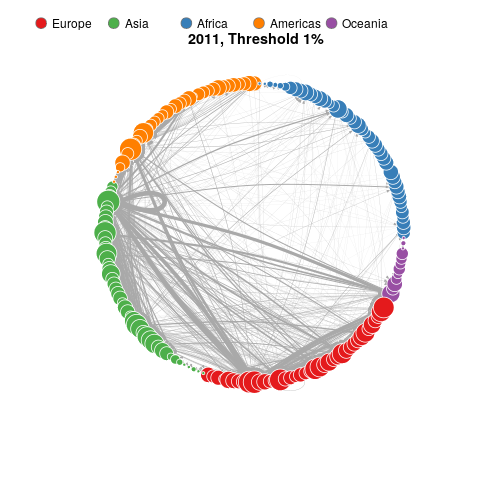
\includegraphics[width=1.4\linewidth]{grafo_Circ_2011_1_pcnt}
\end{figure}

\column{.5\textwidth} % Left column and width
\small

\begin{itemize}

\item[\faRebel] Grafo dirigido no ponderado de \underline{comercio bilateral por año y tipo} 
\item[\faRebel] Análisis de \underline{puntos de corte}
\item[\faRebel] Centralidad de los países
\end{itemize}


\end{columns}
\end{frame}

\begin{frame}
\frametitle{Definición del grafo}

\begin{columns}[t]
\column{.5\textwidth}

$$
a_{ij} = 
\begin{cases} 
1 & si \ \frac{x_{ij}}{x_{i\cdot}}\geq u \\
0 & sino 
\end{cases}
$$
$x_{ij}$: Comercio total entre los países i-j \par
$x_{i\cdot}$: Comercio total del país i

\column{.5\textwidth}

\begin{itemize}[label=\faRebel]
\item Dos países están conectados si existe \textit{suficiente} comercio entre ellos.
\item Puede ser tanto expo como impo.
\item El grafo es dirigido, por lo que $a_{ij} \neq a_{ji}$.
\end{itemize}

\end{columns}

\end{frame}



\begin{frame}
\frametitle{Productores \& Consumidores}	
\begin{columns}
\column{.5\textwidth}
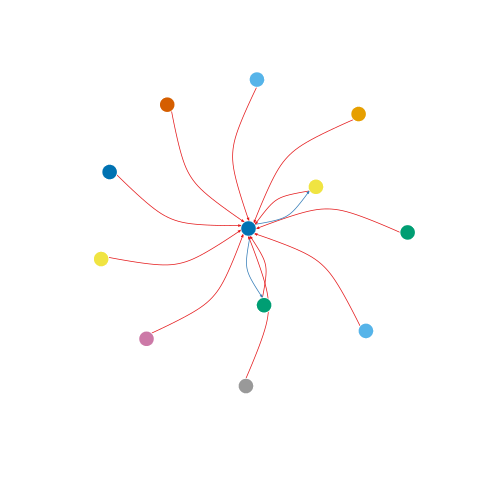
\includegraphics[width=\linewidth]{toy_graph1}

\column{.65\textwidth}
\begin{itemize}[label=\faRebel]
\item Desde el punto de vista de un país, no puede haber muchos países relevantes, $\therefore$ no hay muchas \underline{aristas de salida}
\item Pero puede ser relevante desde el punto de vista de muchos otros países.
$\therefore$ puede recibir muchas \underline{aristas de entrada}
\item Con datos de \underline{expo}, un nodo central es \underline{importante como consumidor}
\item Con datos de \underline{impo}, un nodo central es \underline{importante como productor}
\end{itemize}	
\end{columns}	
\end{frame}

\subsection{Resultados}


\begin{frame}
\centering
\Large Resultados
\end{frame}

\begin{frame}

\scriptsize{
\textbf{Determinación del Punto de corte}. En 1\% Se maximiza el \underline{clustering} y minimiza la \underline{densidad} (dos objetivos deseables para el análisis)}

\begin{figure}
\centering
\subfigure[1\%]{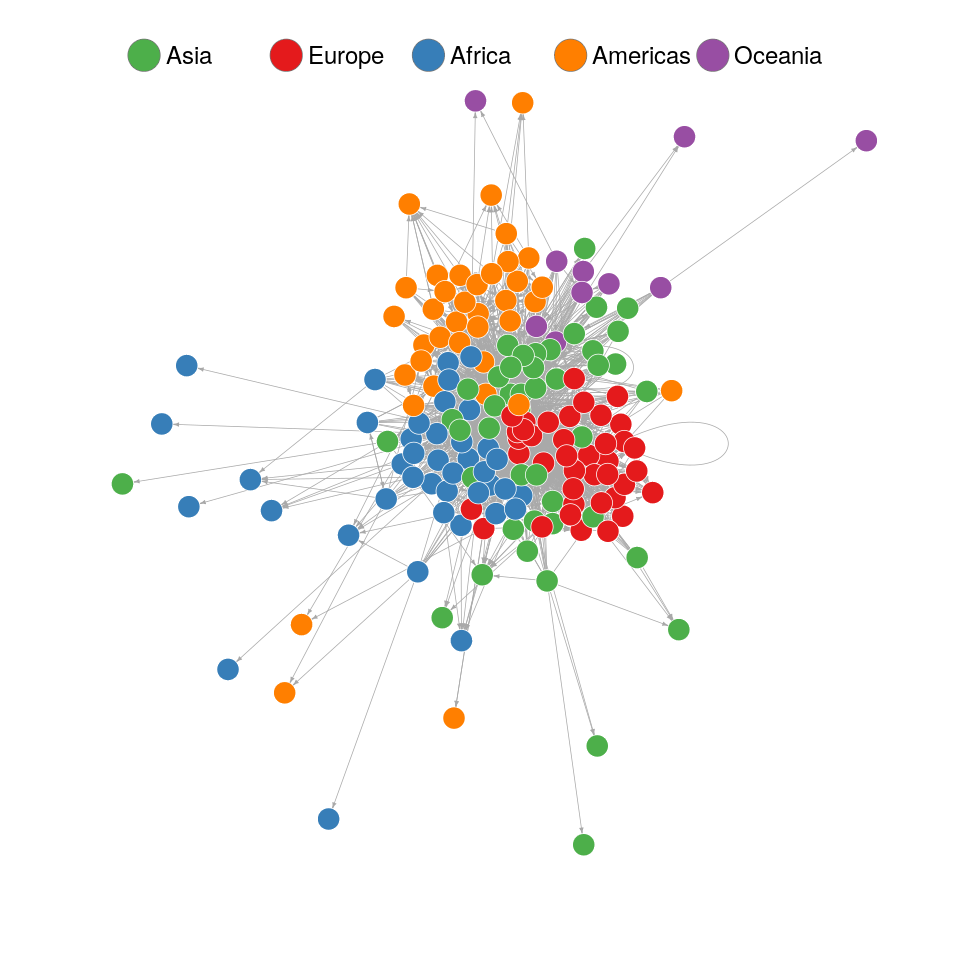
\includegraphics[width=0.2\linewidth]{grafo_2016_1_pcnt}}
\subfigure[5\%]{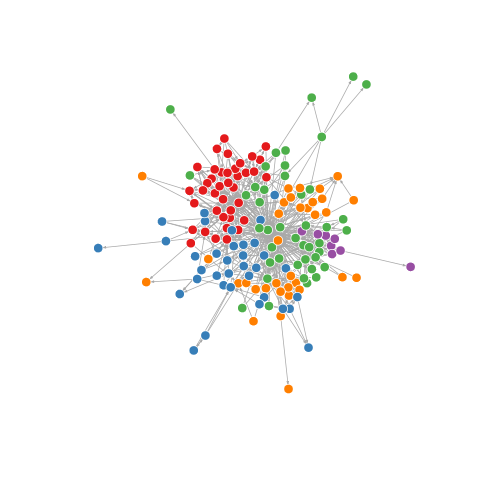
\includegraphics[width=0.2\linewidth]{grafo_2016_5_pcnt}}
\subfigure[10\%]{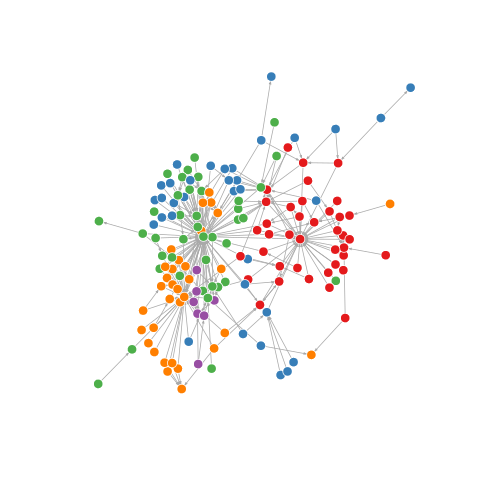
\includegraphics[width=0.2\linewidth]{grafo_2016_10_pcnt}}
\subfigure[15\%]{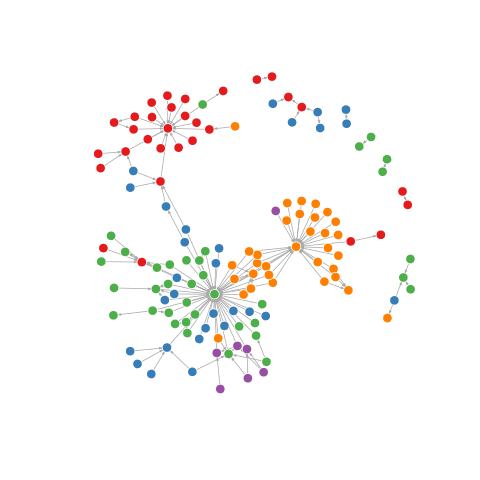
\includegraphics[width=0.2\linewidth]{grafo_2016_15_pcnt}}
\subfigure[20\%]{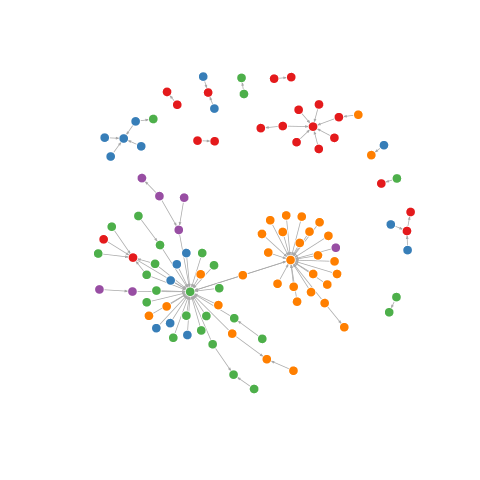
\includegraphics[width=0.2\linewidth]{grafo_2016_20_pcnt}}
\subfigure[25\%]{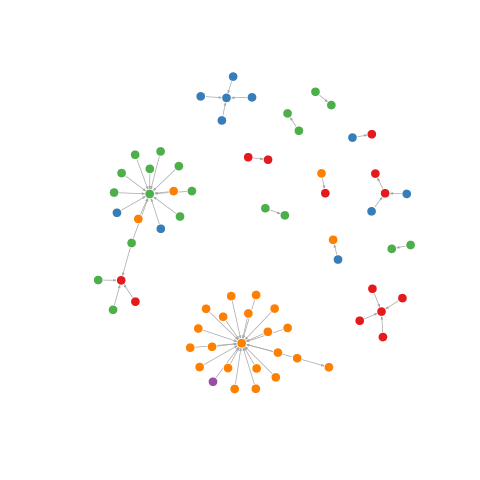
\includegraphics[width=0.2\linewidth]{grafo_2016_25_pcnt}}
\subfigure[Clustering]{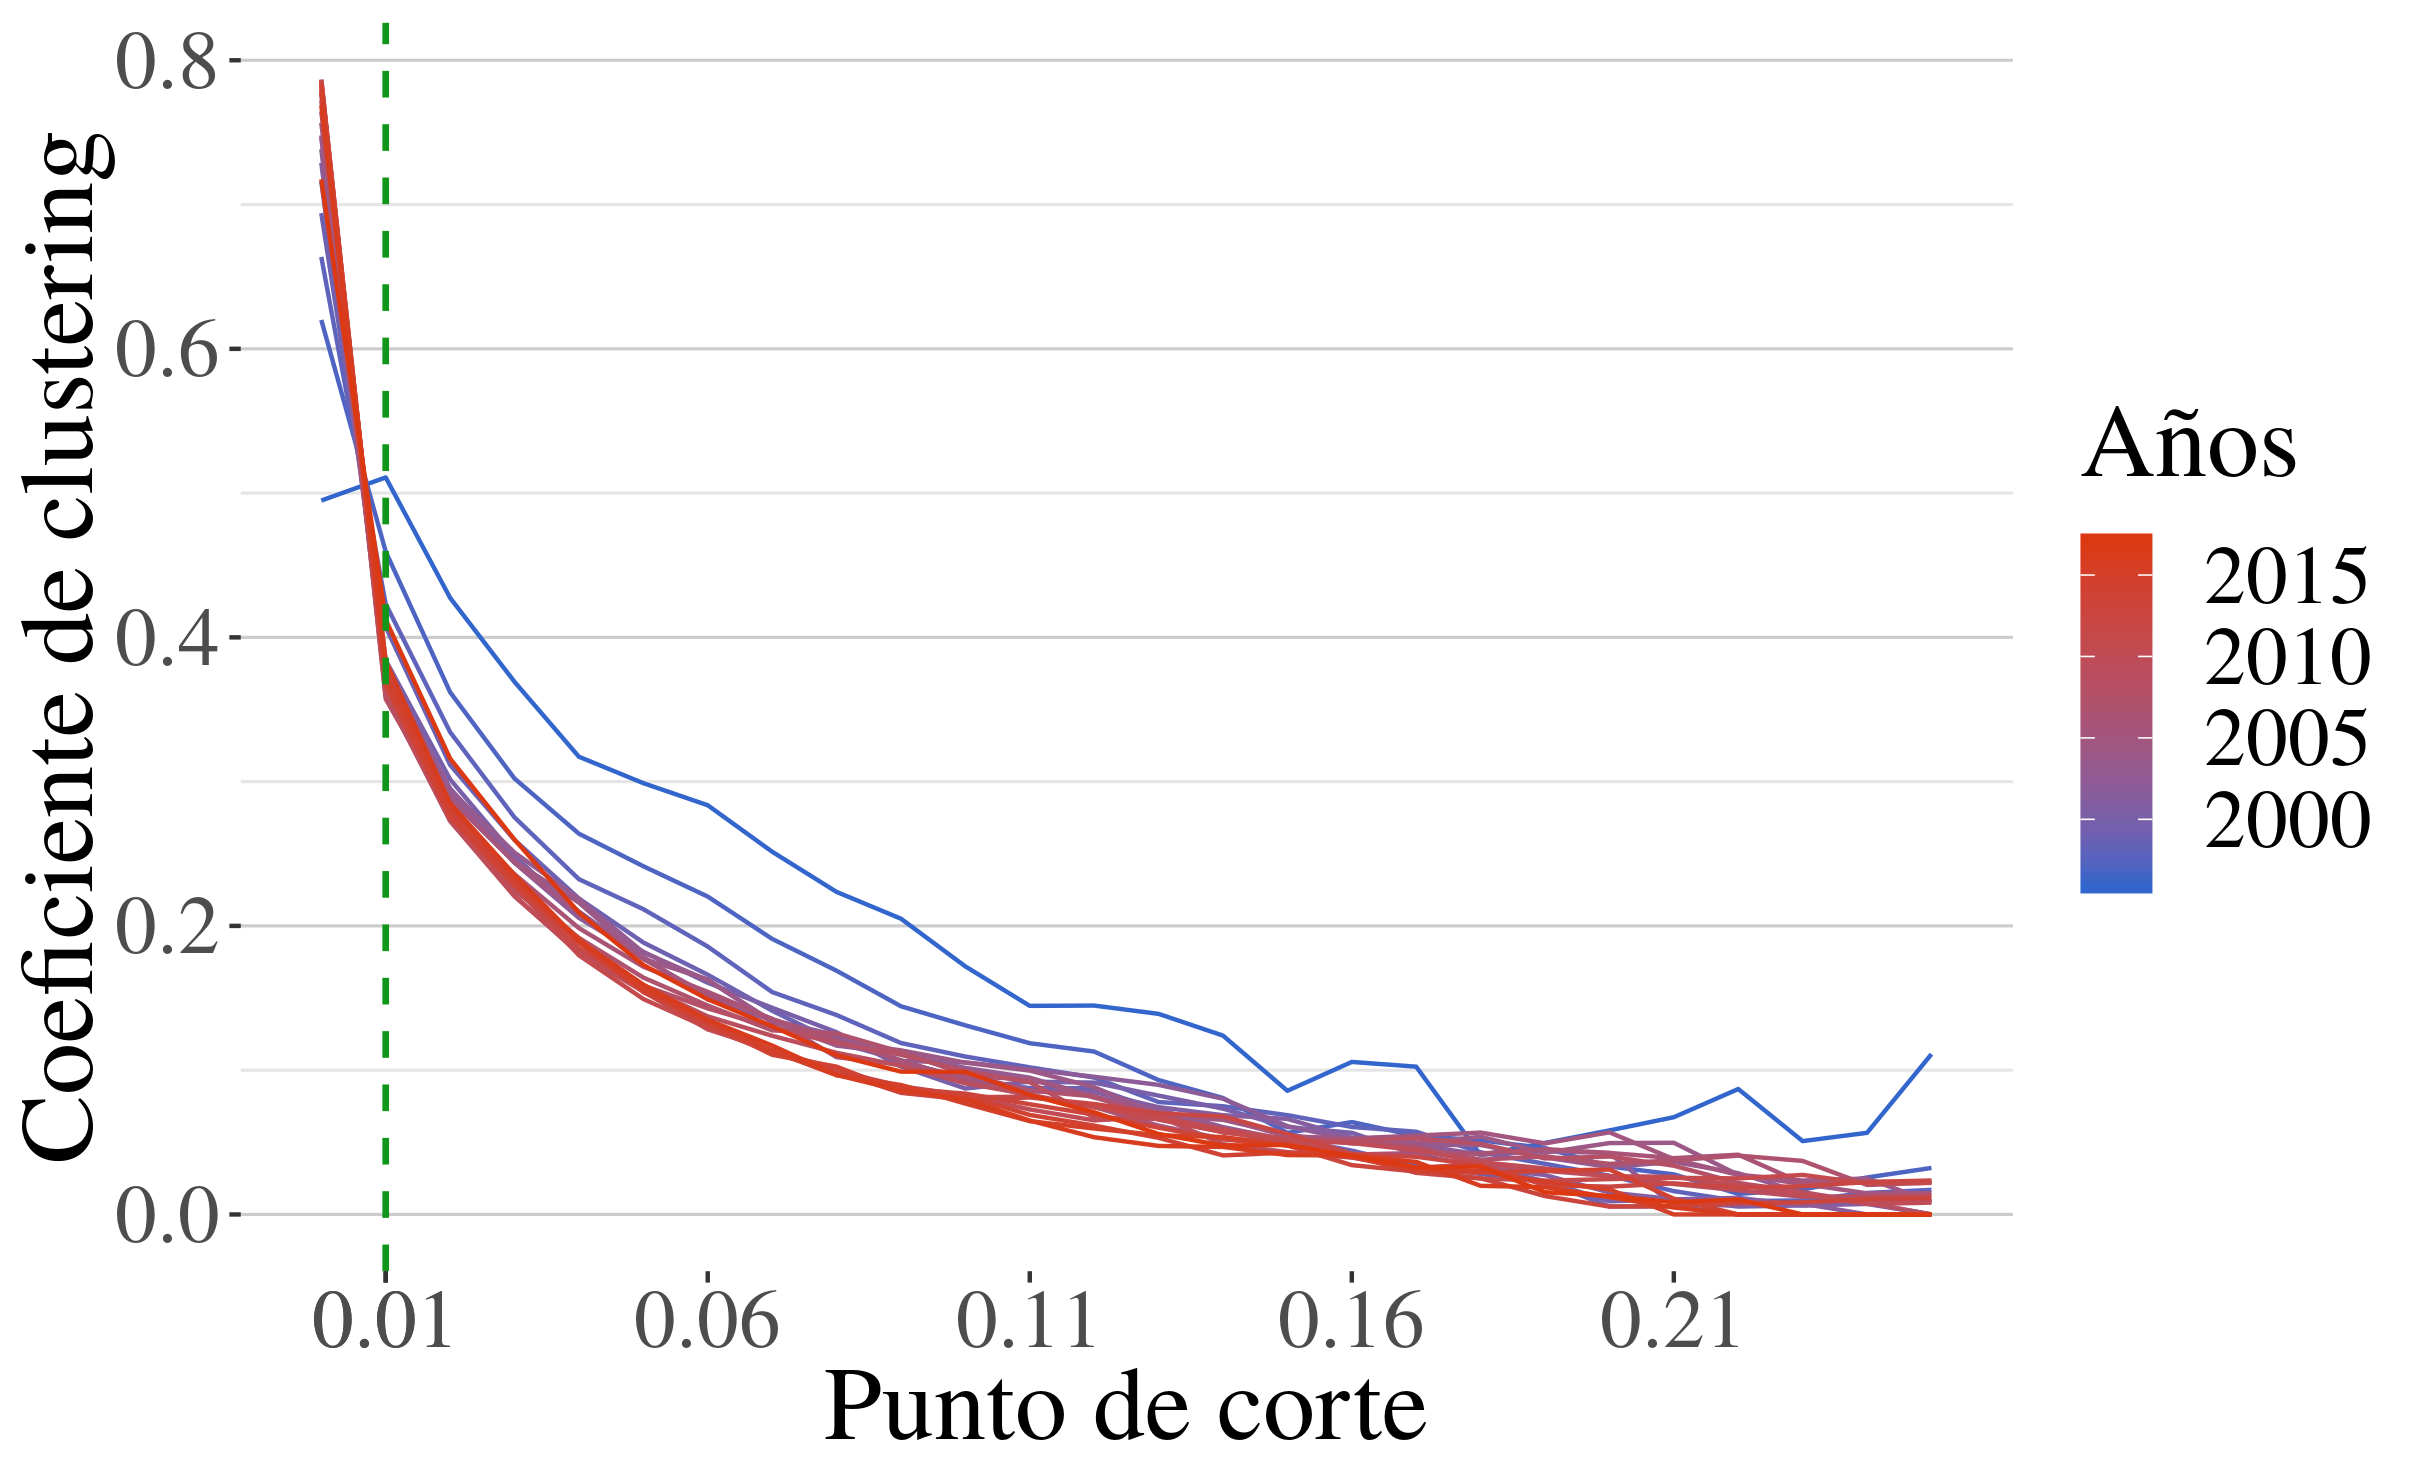
\includegraphics[width=0.4\linewidth]{threshold_x_clustering_x_yr}}
\caption{Grafos. 2016, según punto de corte}
\label{fig:grafo_2016}
\end{figure}

\end{frame}



\begin{frame}

%The relation of the centrality measures between exports and imports networks for a given year shows the relative position in word trade of the countries/continents	

\frametitle{Correlación Expo-Impo.}

punto de corte: 1\%.
Coeficiente de Pearson= 0.96

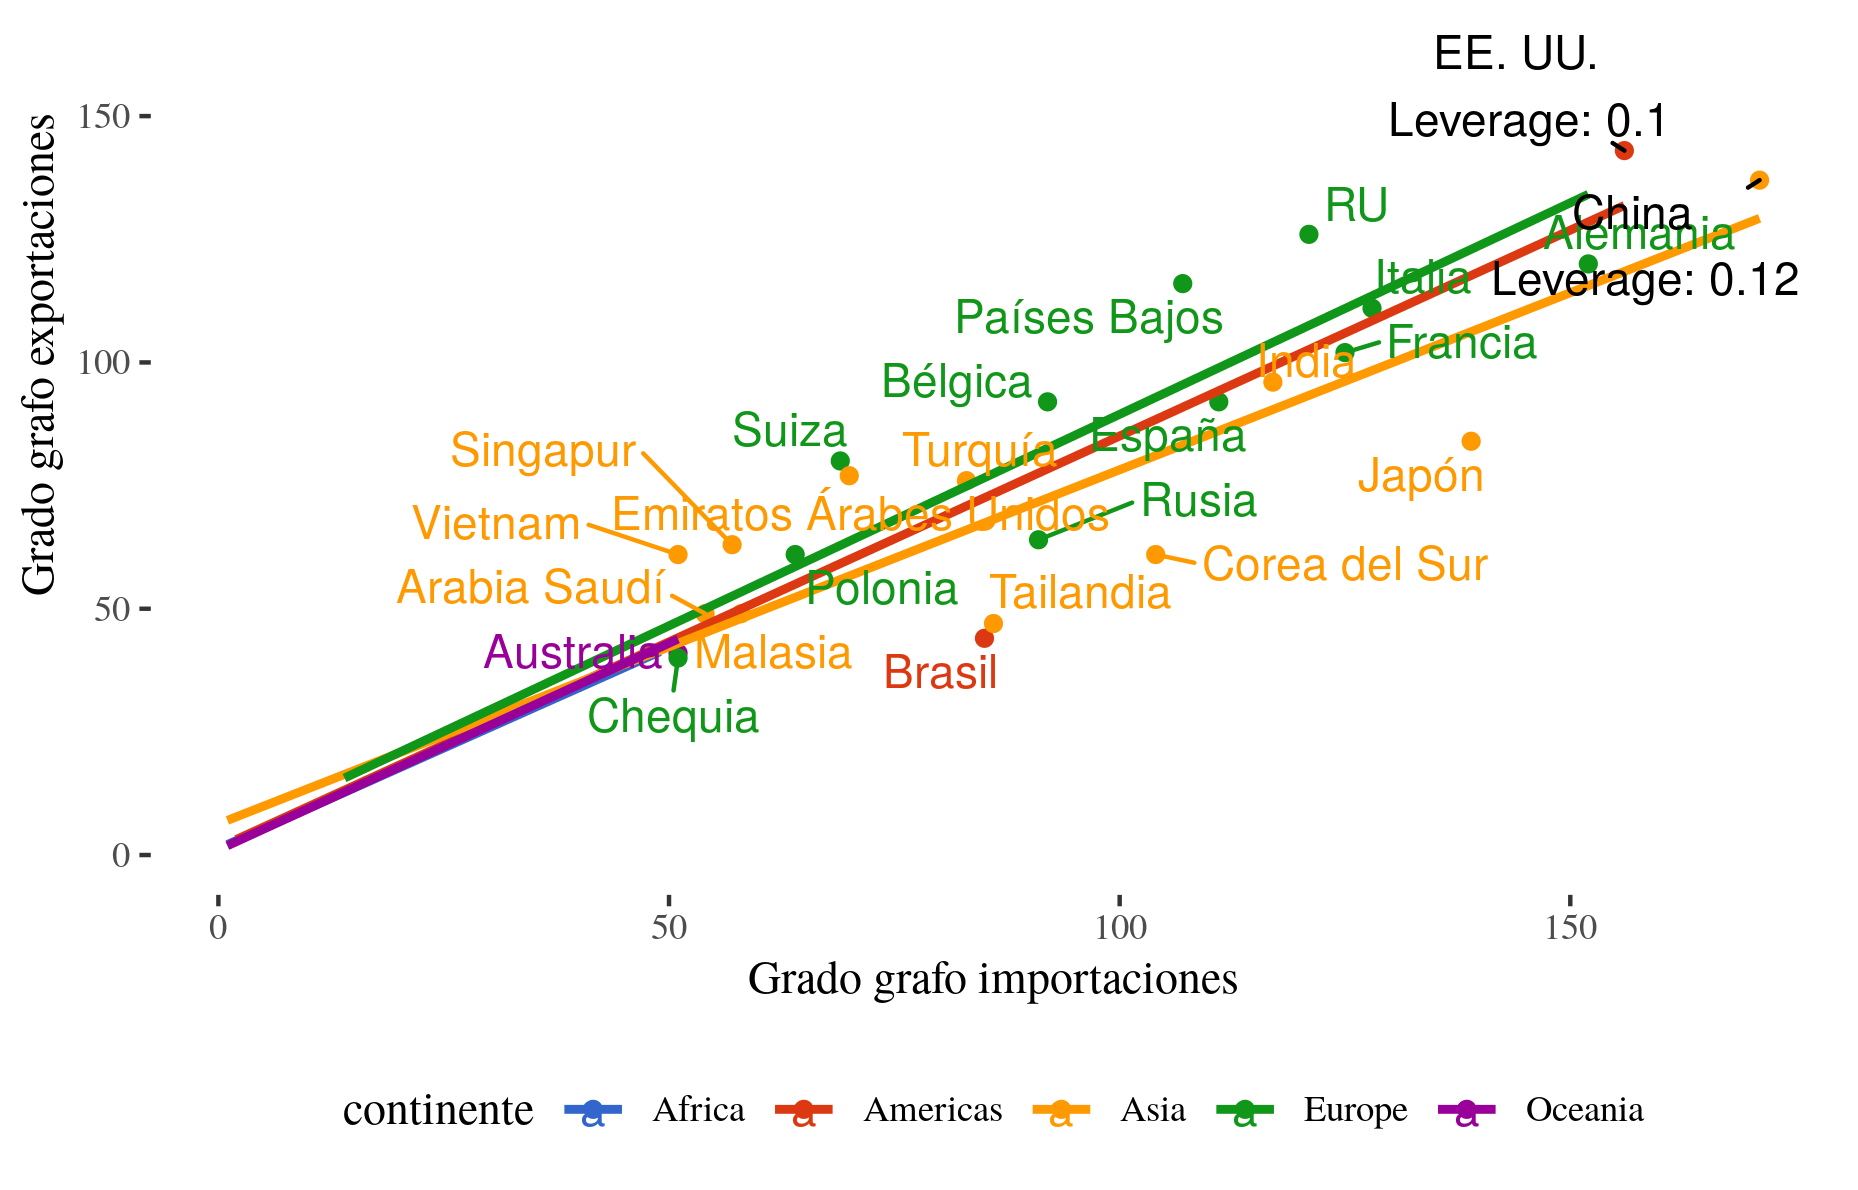
\includegraphics[width=\linewidth]{Graficos/corr_grados_2016_1_pcnt}

\end{frame}

\begin{frame}

\begin{itemize}
\item[\faRebel] Por la forma de construcción, una mayor centralidad en el grafo de las \underline{importaciones} denota una importancia del país como \underline{productor para el mercado mundial}, y viceversa.
\item[\faRebel] Podemos ver que hay una \underline{correlación alta} entre ambos grafos, pero también que países como Bélgica o Suiza son más importantes como \underline{consumidores} de mercancías.
\item[\faRebel] Corea del Sur, Japón y Brasil, por su parte, son más importantes como \underline{productores} de mercancías. 
\end{itemize}
\end{frame}


\begin{frame}
\frametitle{Correlación Expo-Impo.}

punto de corte: 10\%.
Coeficiente de Pearson= 0.77

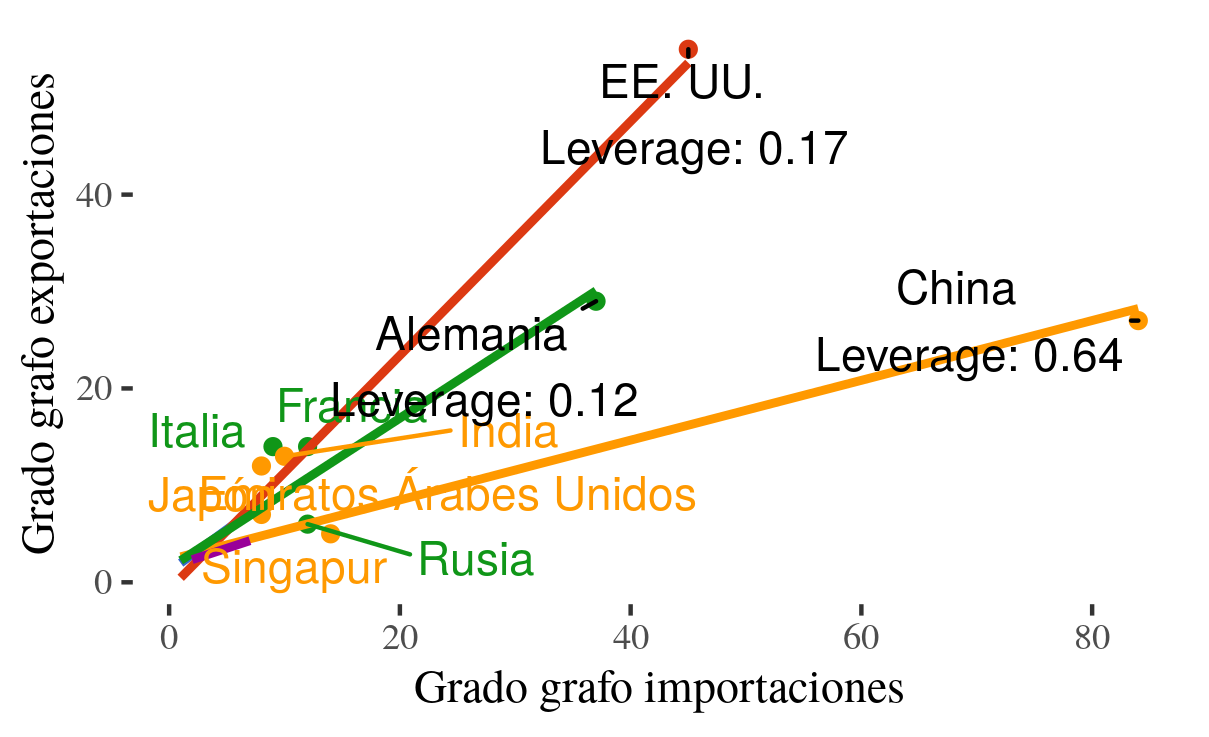
\includegraphics[width=\linewidth]{Graficos/corr_grados_2016_10_pcnt}

\end{frame}

\begin{frame}

\begin{itemize}
\item[\faRebel] Un punto de corte más alto implica relaciones de mayor dependencia.\\

\item[\faRebel] En este tipo de relaciones destacan menos países, con mayor leverage 
\end{itemize}
\end{frame}


\begin{frame}
\frametitle{Correlación Expo-Impo.}

punto de corte: 20\%.
Coeficiente de Pearson= 0.81

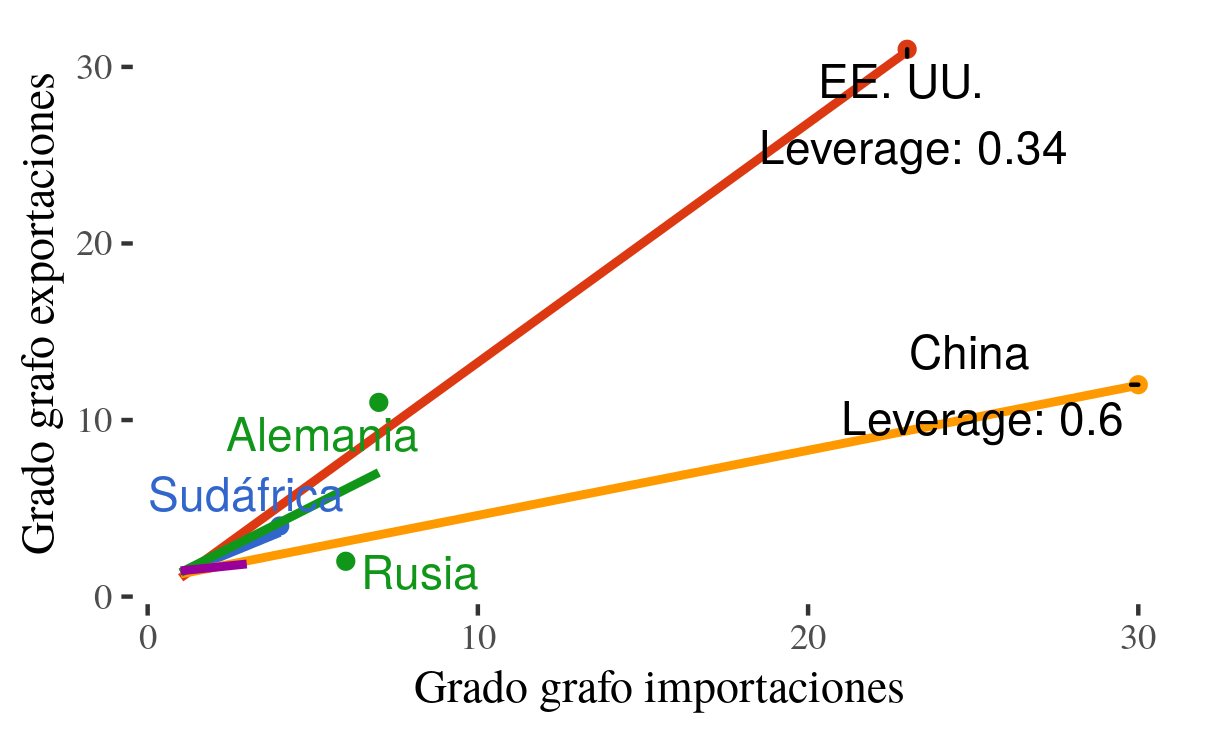
\includegraphics[width=\linewidth]{Graficos/corr_grados_2016_20_pcnt}

\end{frame}

\begin{frame}

\begin{itemize}
\item[\faRebel] En el extremo, en relaciones de \underline{alta dependencia} destacan sobretodo Estados Unidos como consumidor, y China como productor.
\item[\faRebel] Alemania, Sudáfrica y Rusia también destacan por tener relaciones de alta dependencia. 
\end{itemize}
\end{frame}



\begin{frame}
\begin{figure}

\centering
\subfigure{\label{fig:metricas_LP-a}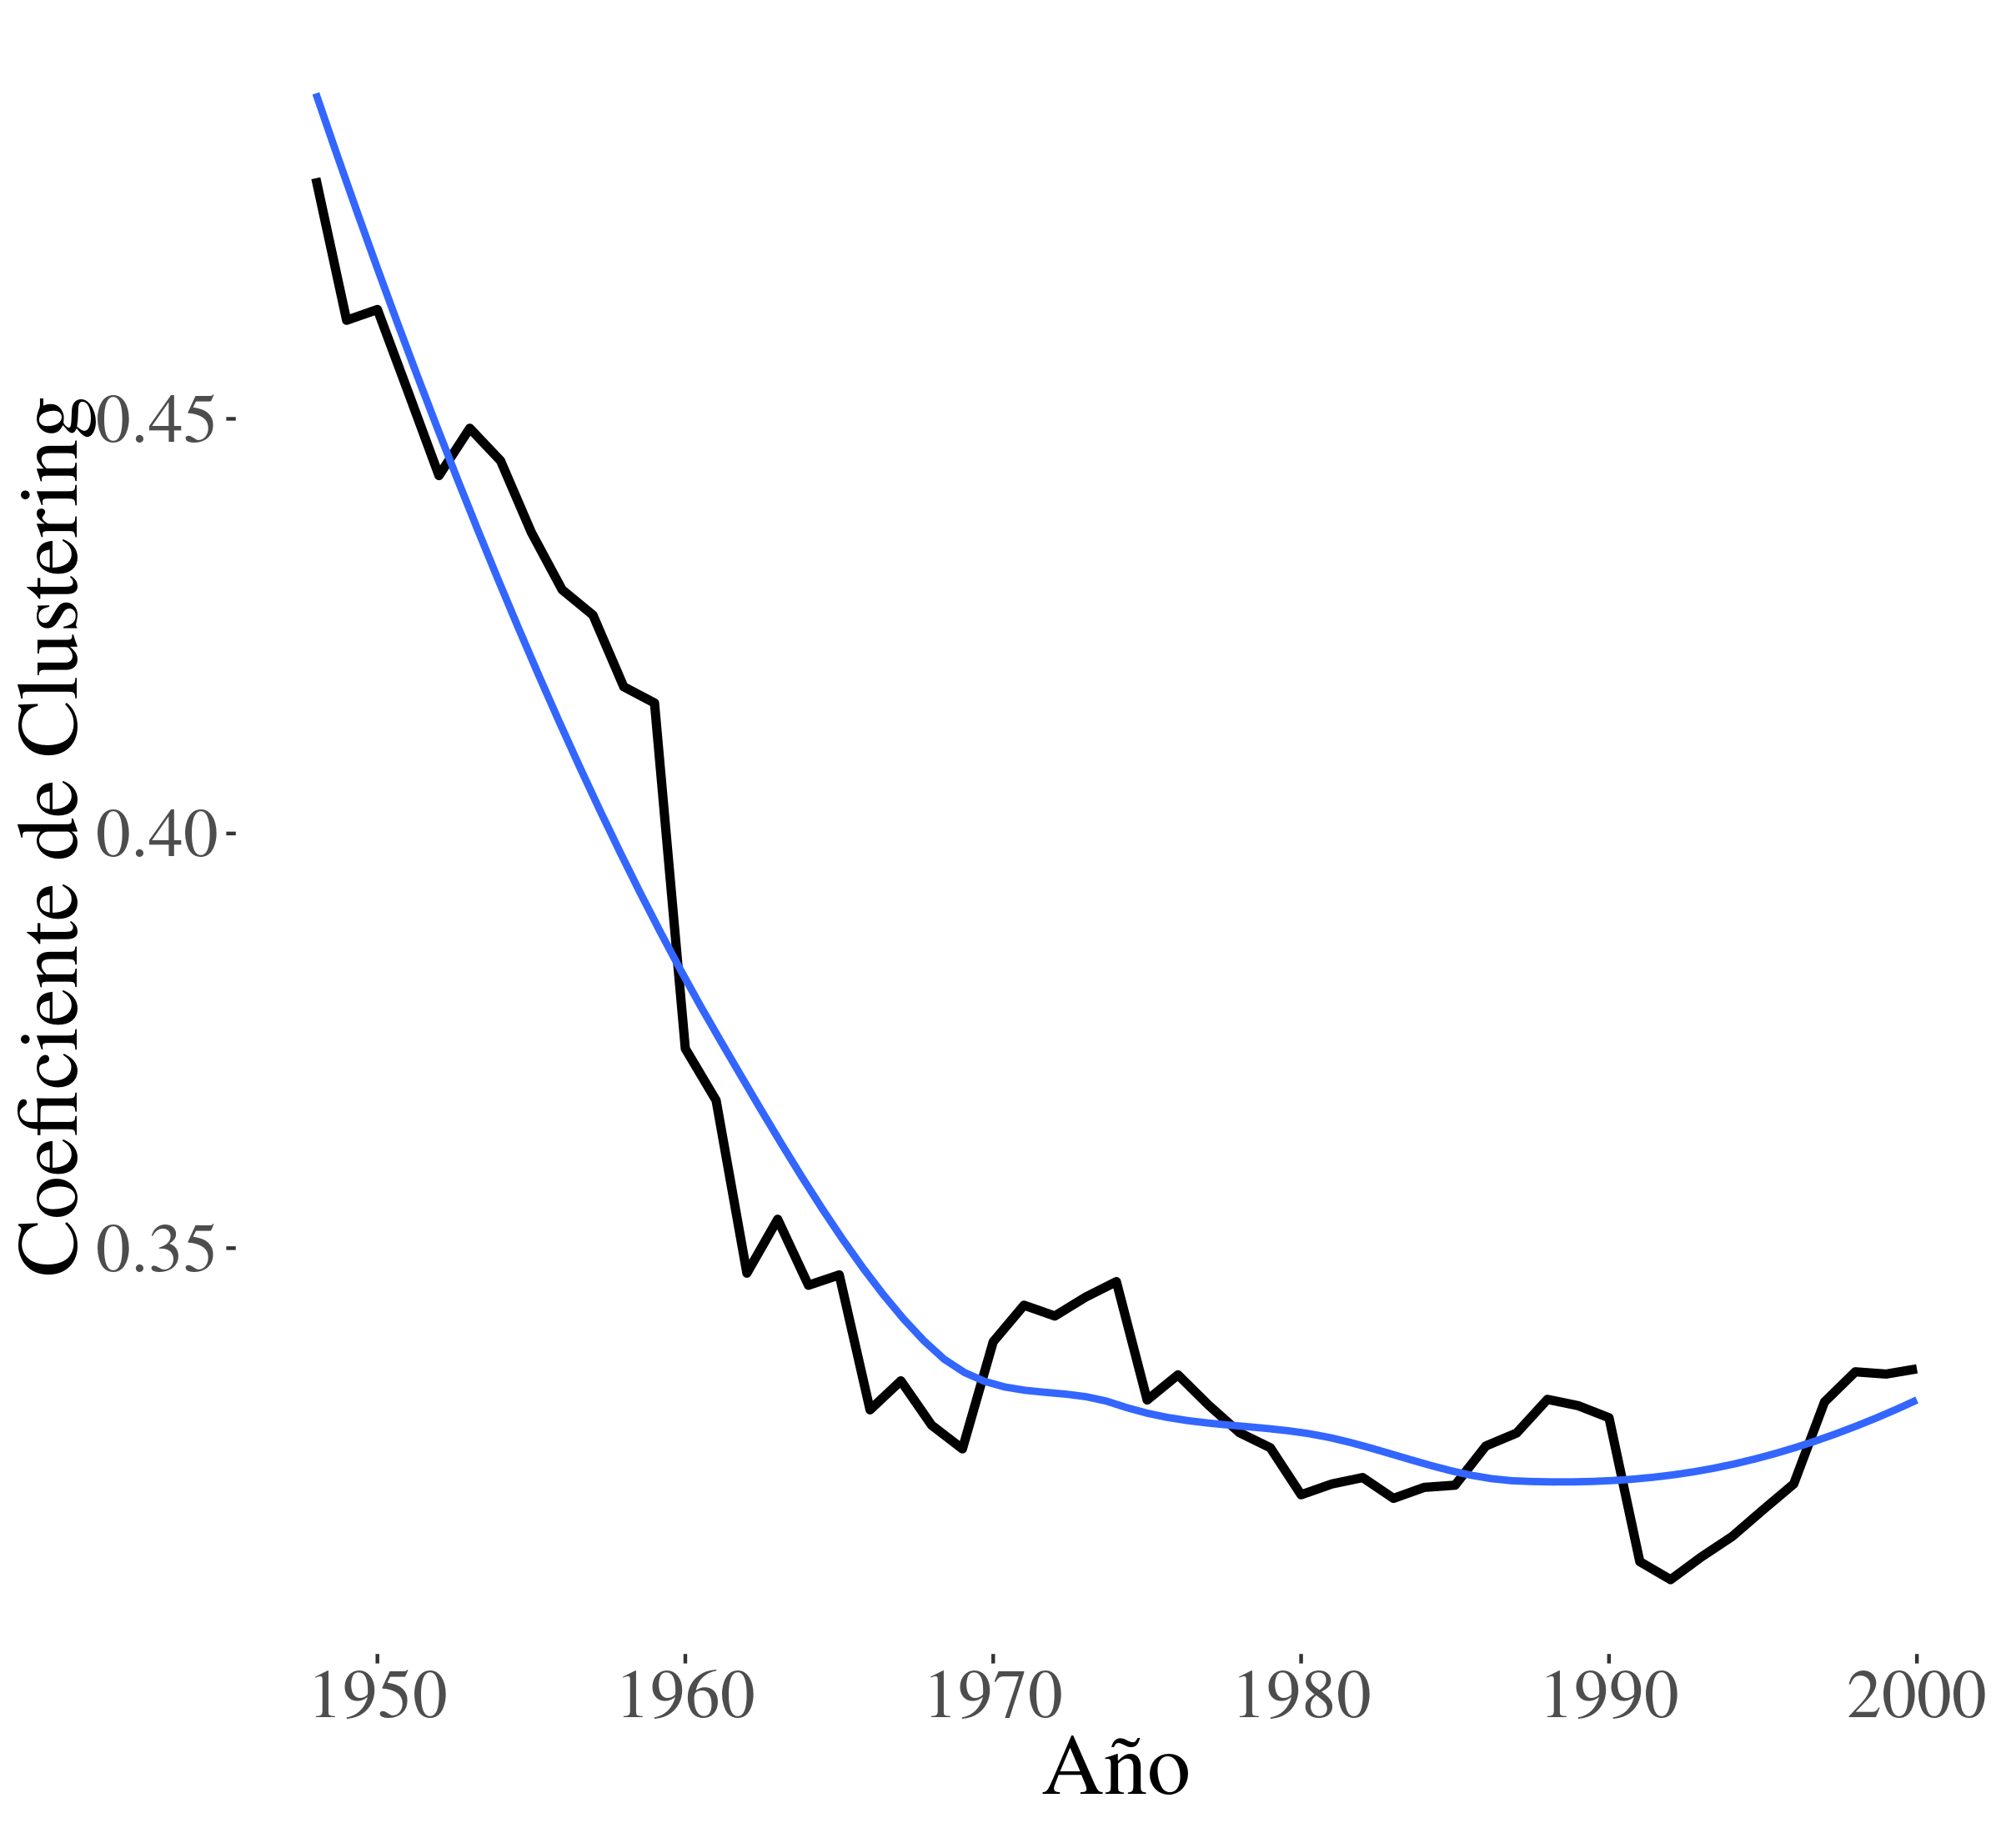
\includegraphics[width=.48\linewidth]{1950_2000_coef_clustering_x_yr}}
\subfigure{\label{fig:metricas_LP-b}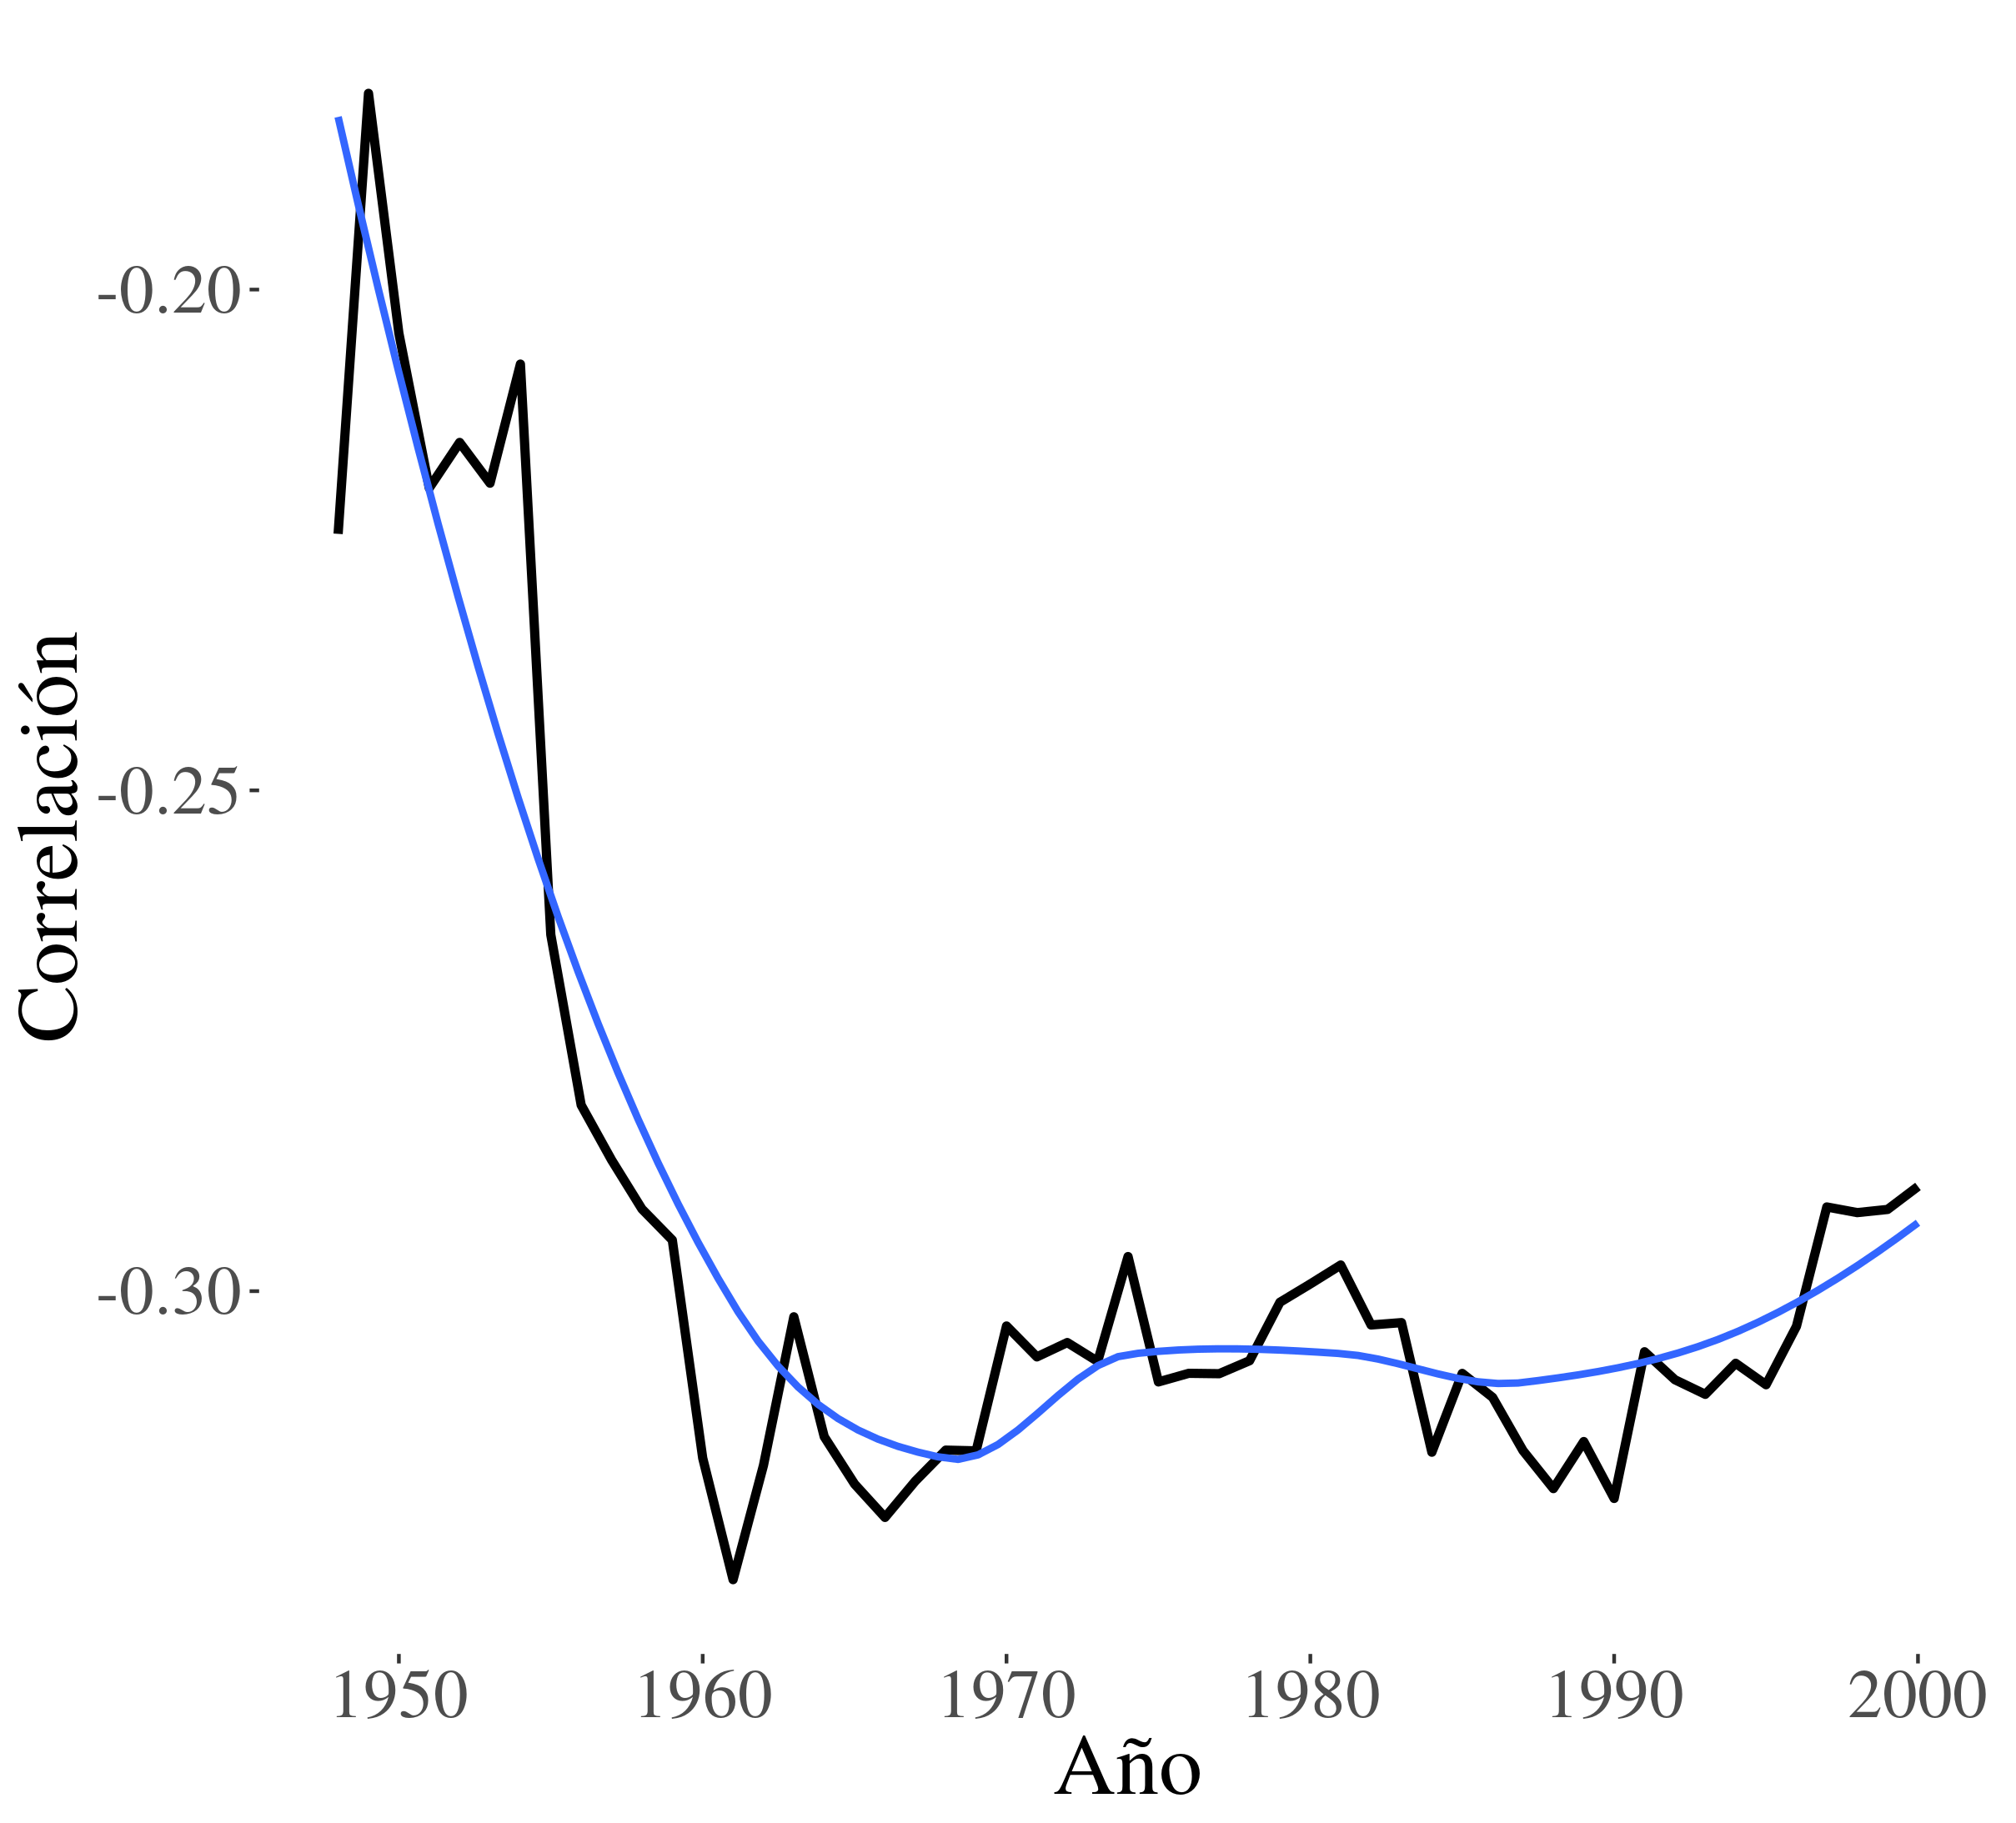
\includegraphics[width=.48\linewidth]{1950_2000_correlacion_x_yr}}
\caption*{\scriptsize Evolución de la estructura de la red. Importaciones. Umbral 1\%. 1948-2000}
\label{fig:metricas_LP}
\end{figure}

\small
\begin{itemize}[label=\faRebel]
\item En la segunda mitad del S XX se observa una tendencia a la clusterización o \underline{regionalización de las relaciones comerciales}.
\item La caída de la correlación de grado indica un aumento de las relaciones entre países \underline{centrales} y \underline{periféricos}
\end{itemize}


\end{frame}

\begin{frame}
\begin{figure}
\centering		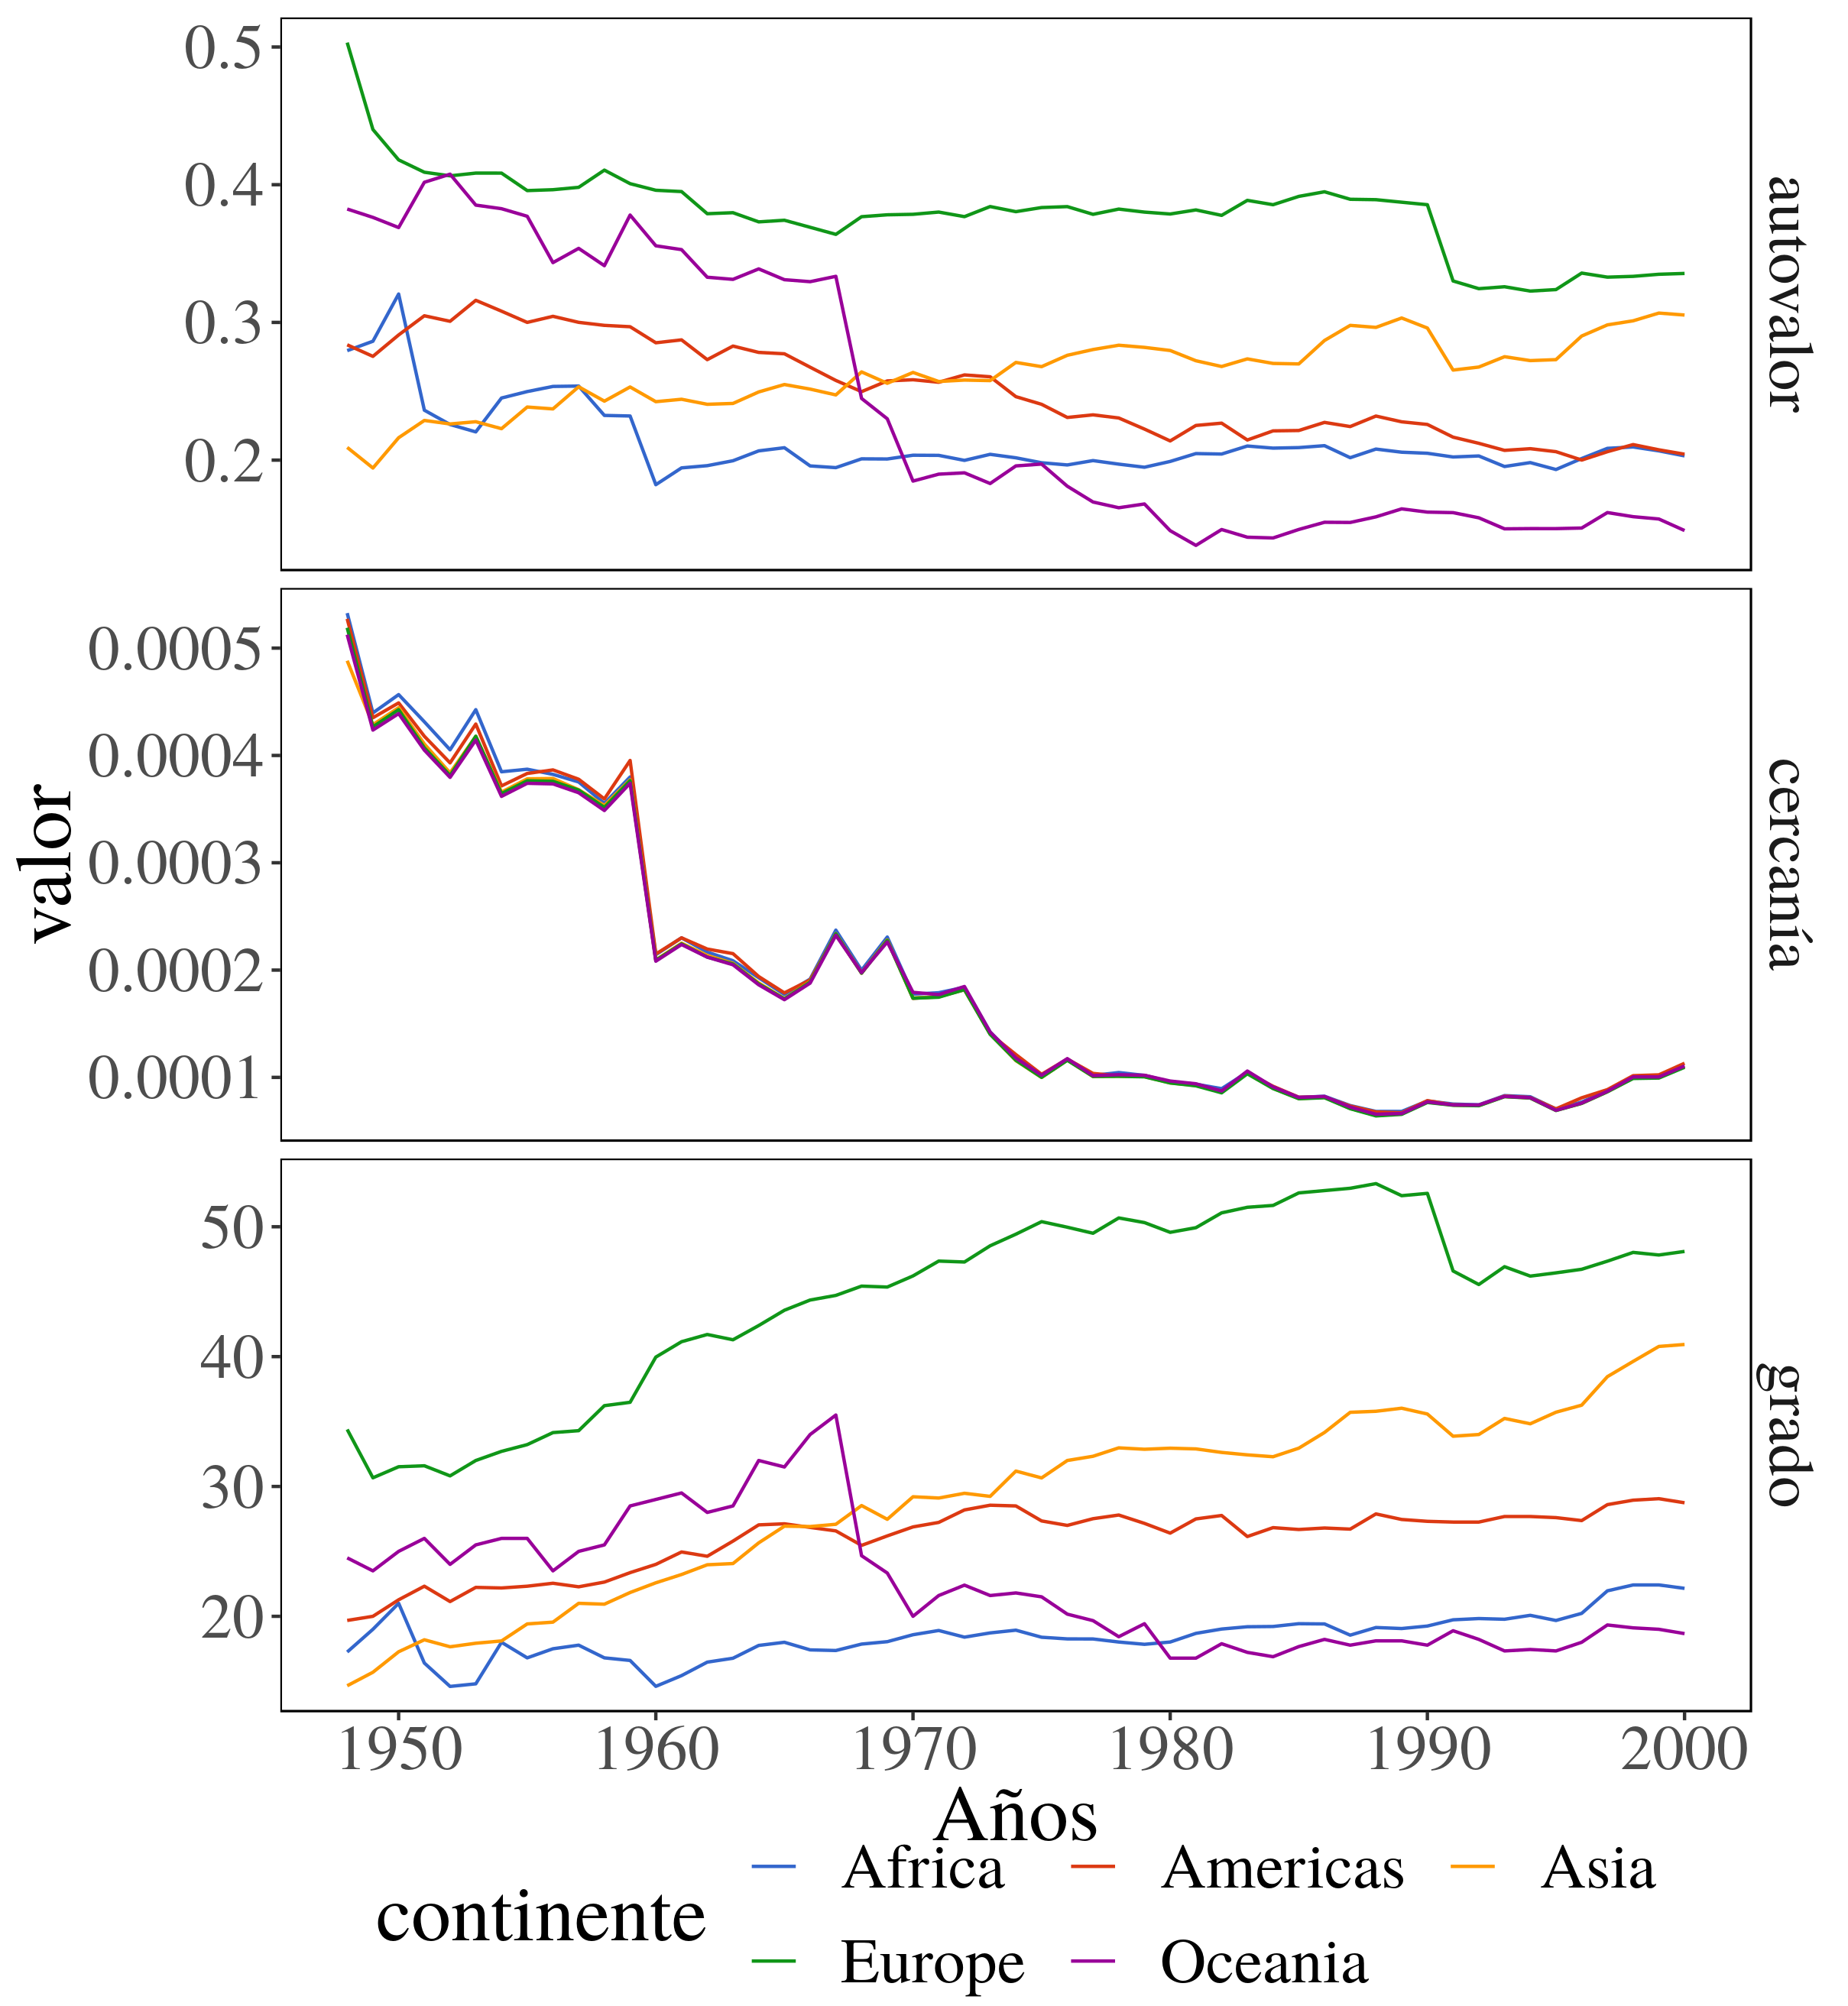
\includegraphics[width=0.75\linewidth]{1950_2000_continent_all}
\caption{Evolución de la centralidad promedio por contiente. Impo. Umbral 1\%}
\label{fig:centralidad_LP}
\end{figure}
\end{frame}

\begin{frame}
\begin{itemize}[label=\faRebel]
\item Tanto en la centralidad de autovalor como en la de grado, \underline{Asia} pasa del último lugar al segundo. 
\item En la centralidad de \underline{cercanía} podemos observar que cae a lo largo de la serie de igual manera en todos los continentes.
\end{itemize}
\end{frame}

\begin{frame}	
\small{Evolución de la distribución de la centralidad de grado en el tiempo. China y EEUU destacado}

\begin{columns}[c] 


\column{.45\textwidth} % Right column and width
\begin{figure}
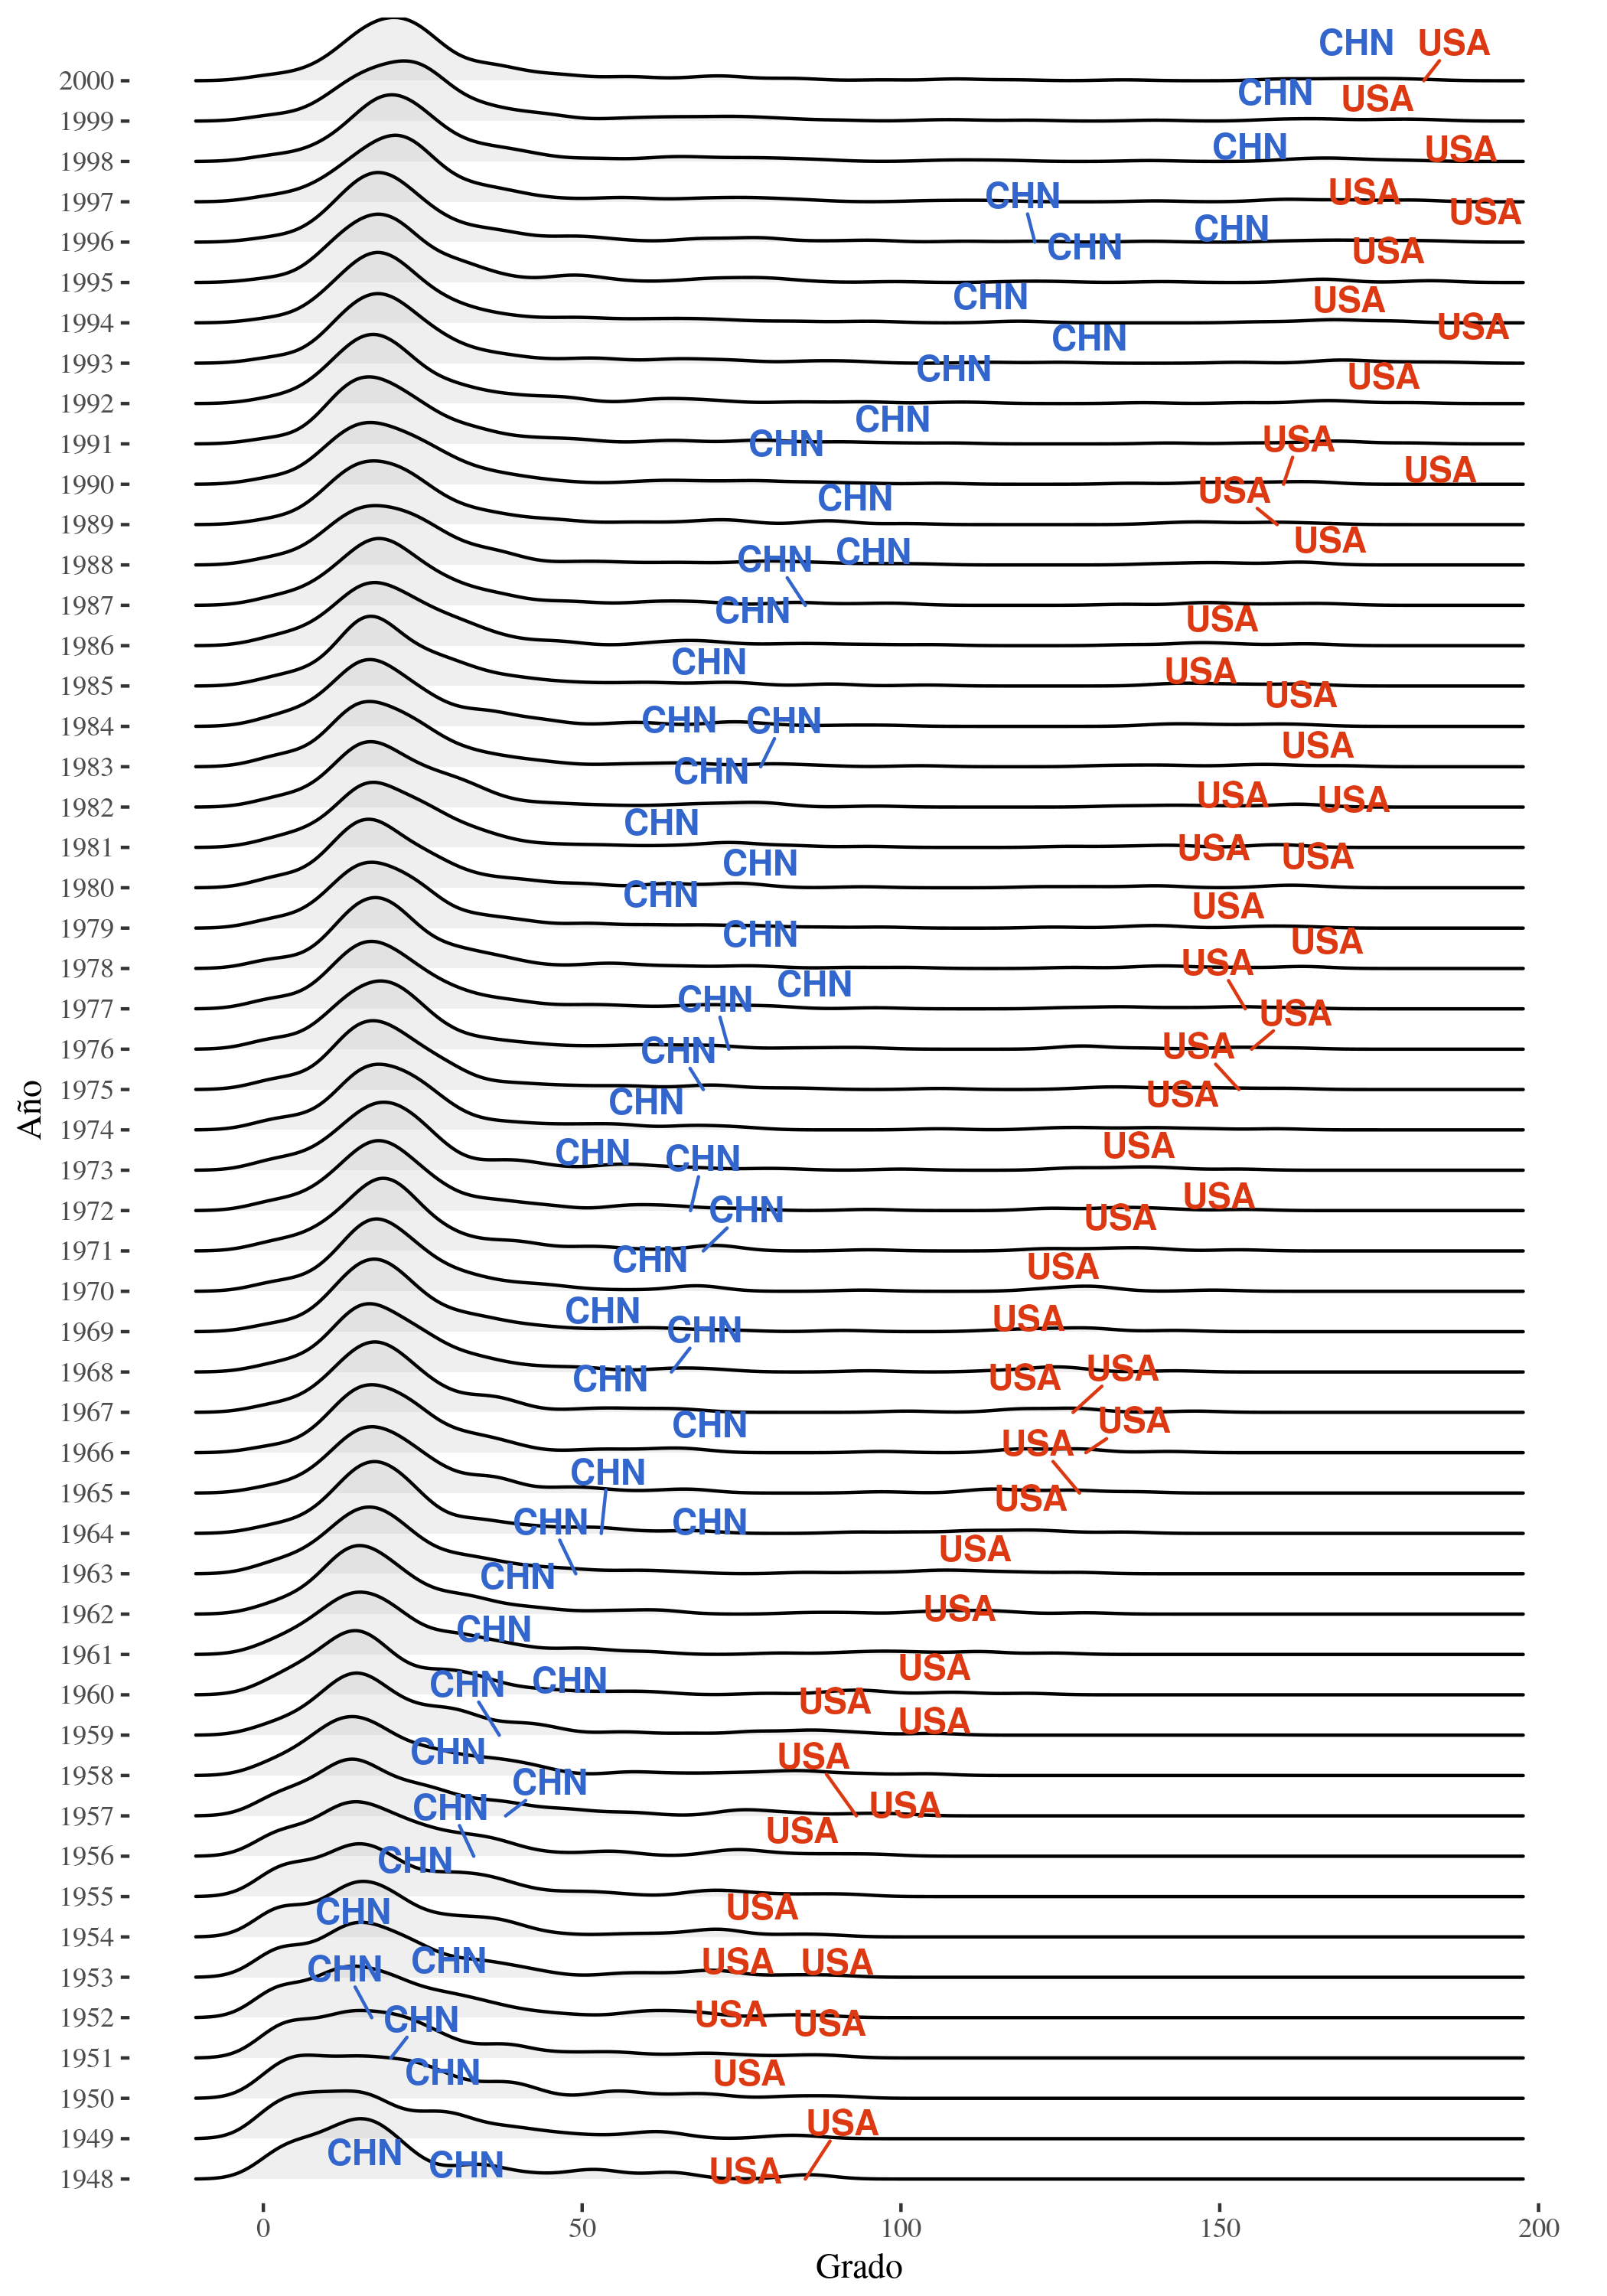
\includegraphics[scale=0.25]{1950_2000_impo_densidad_USA_CHN_grado}
\end{figure}

\column{.5\textwidth} % Left column and width

\begin{flushleft}
\begin{figure}
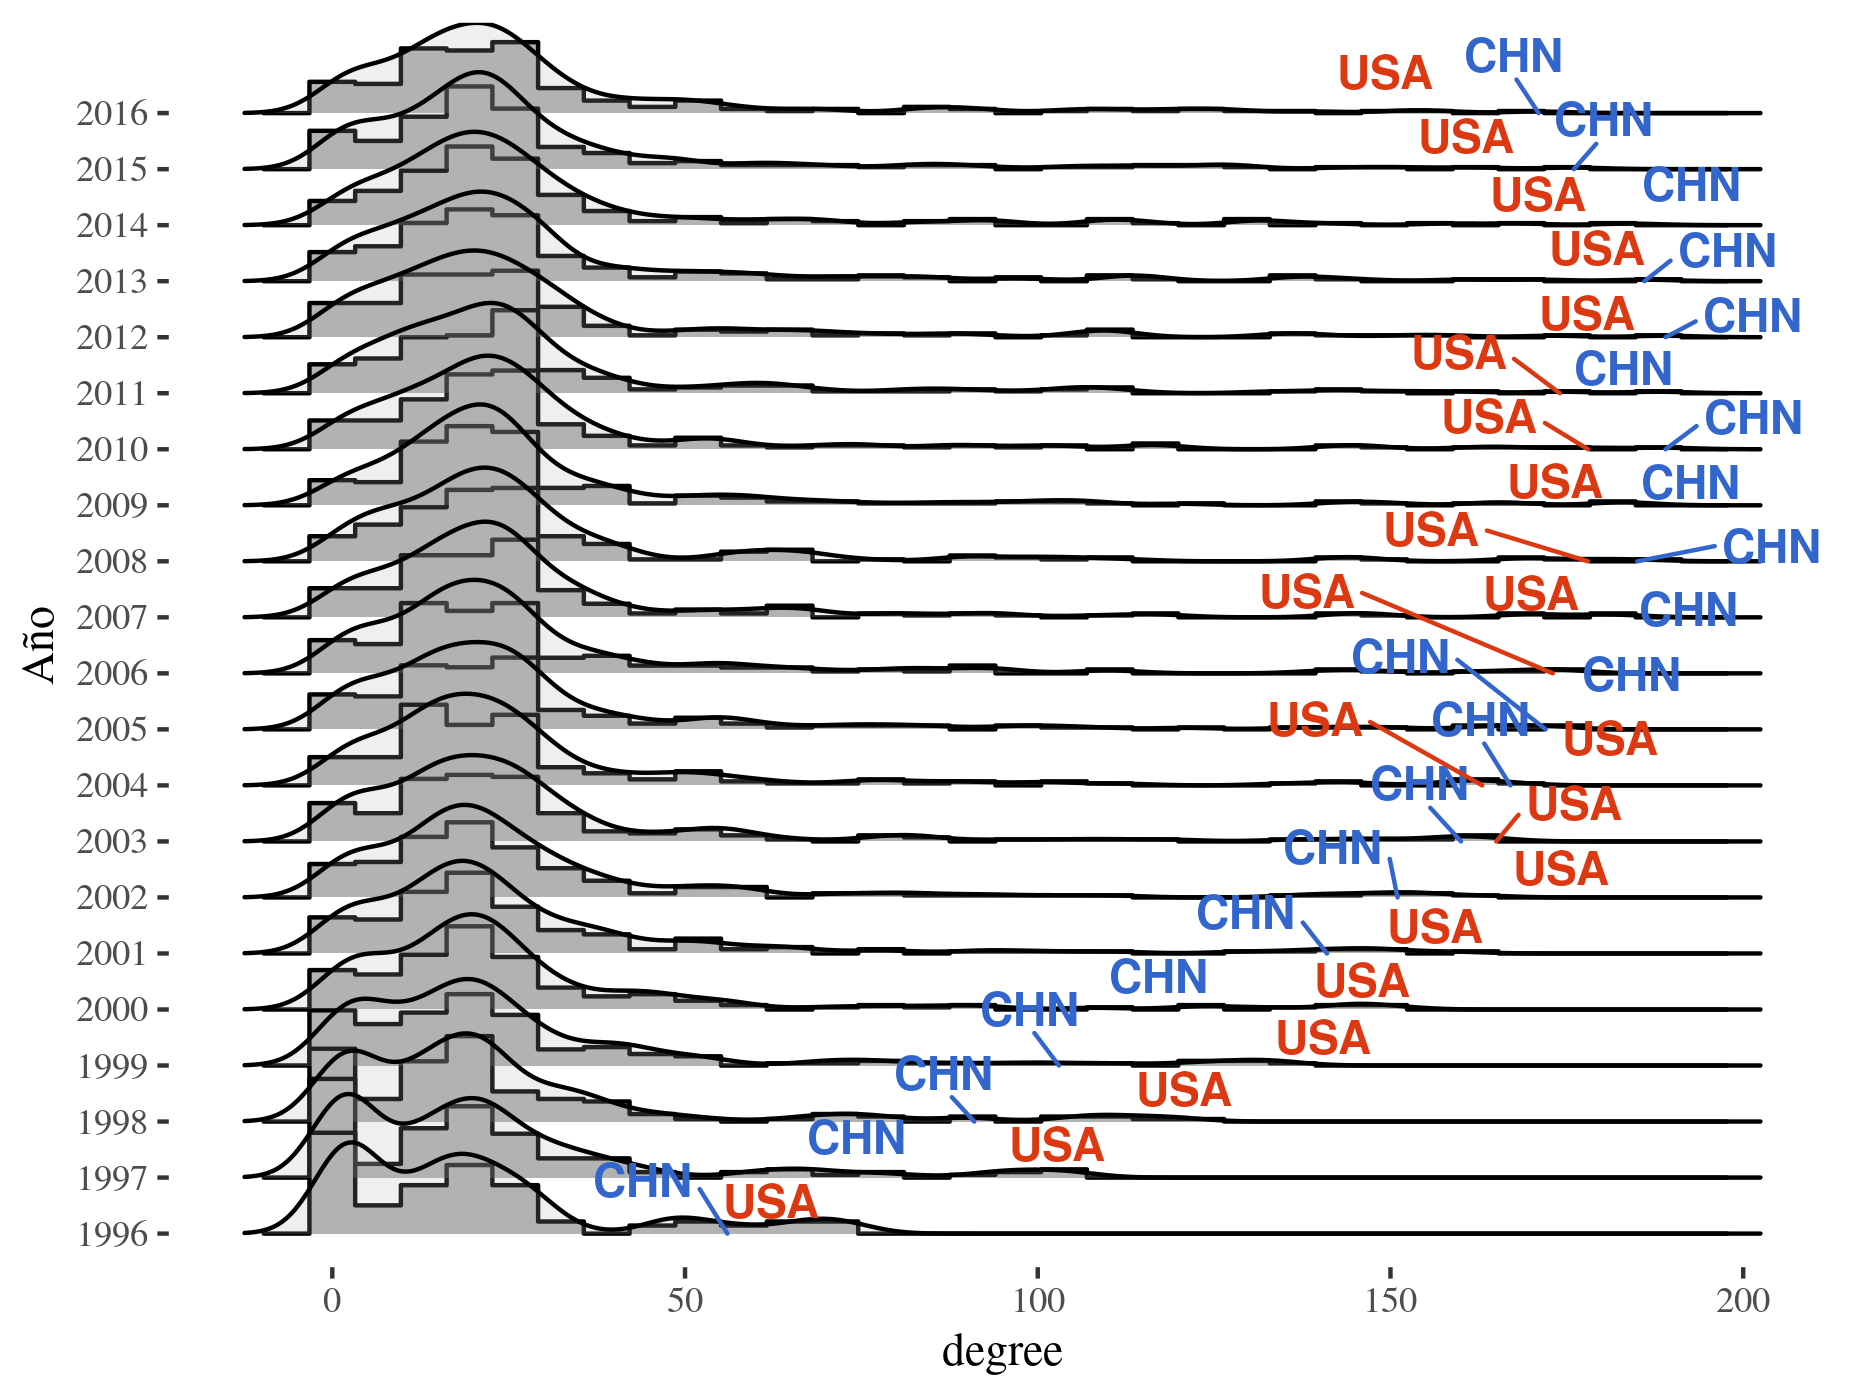
\includegraphics[scale=0.35]{impo_densidad_USAvsCHN_grado_x_yr}
\end{figure}
\end{flushleft}

\end{columns}
\end{frame}


\begin{frame}	
\small{Evolución de la distribución de la centralidad de autovalor en el tiempo. Japón, Corea del Sur y China destacado}

\begin{columns}[c] 
\column{.45\textwidth}
\begin{figure}
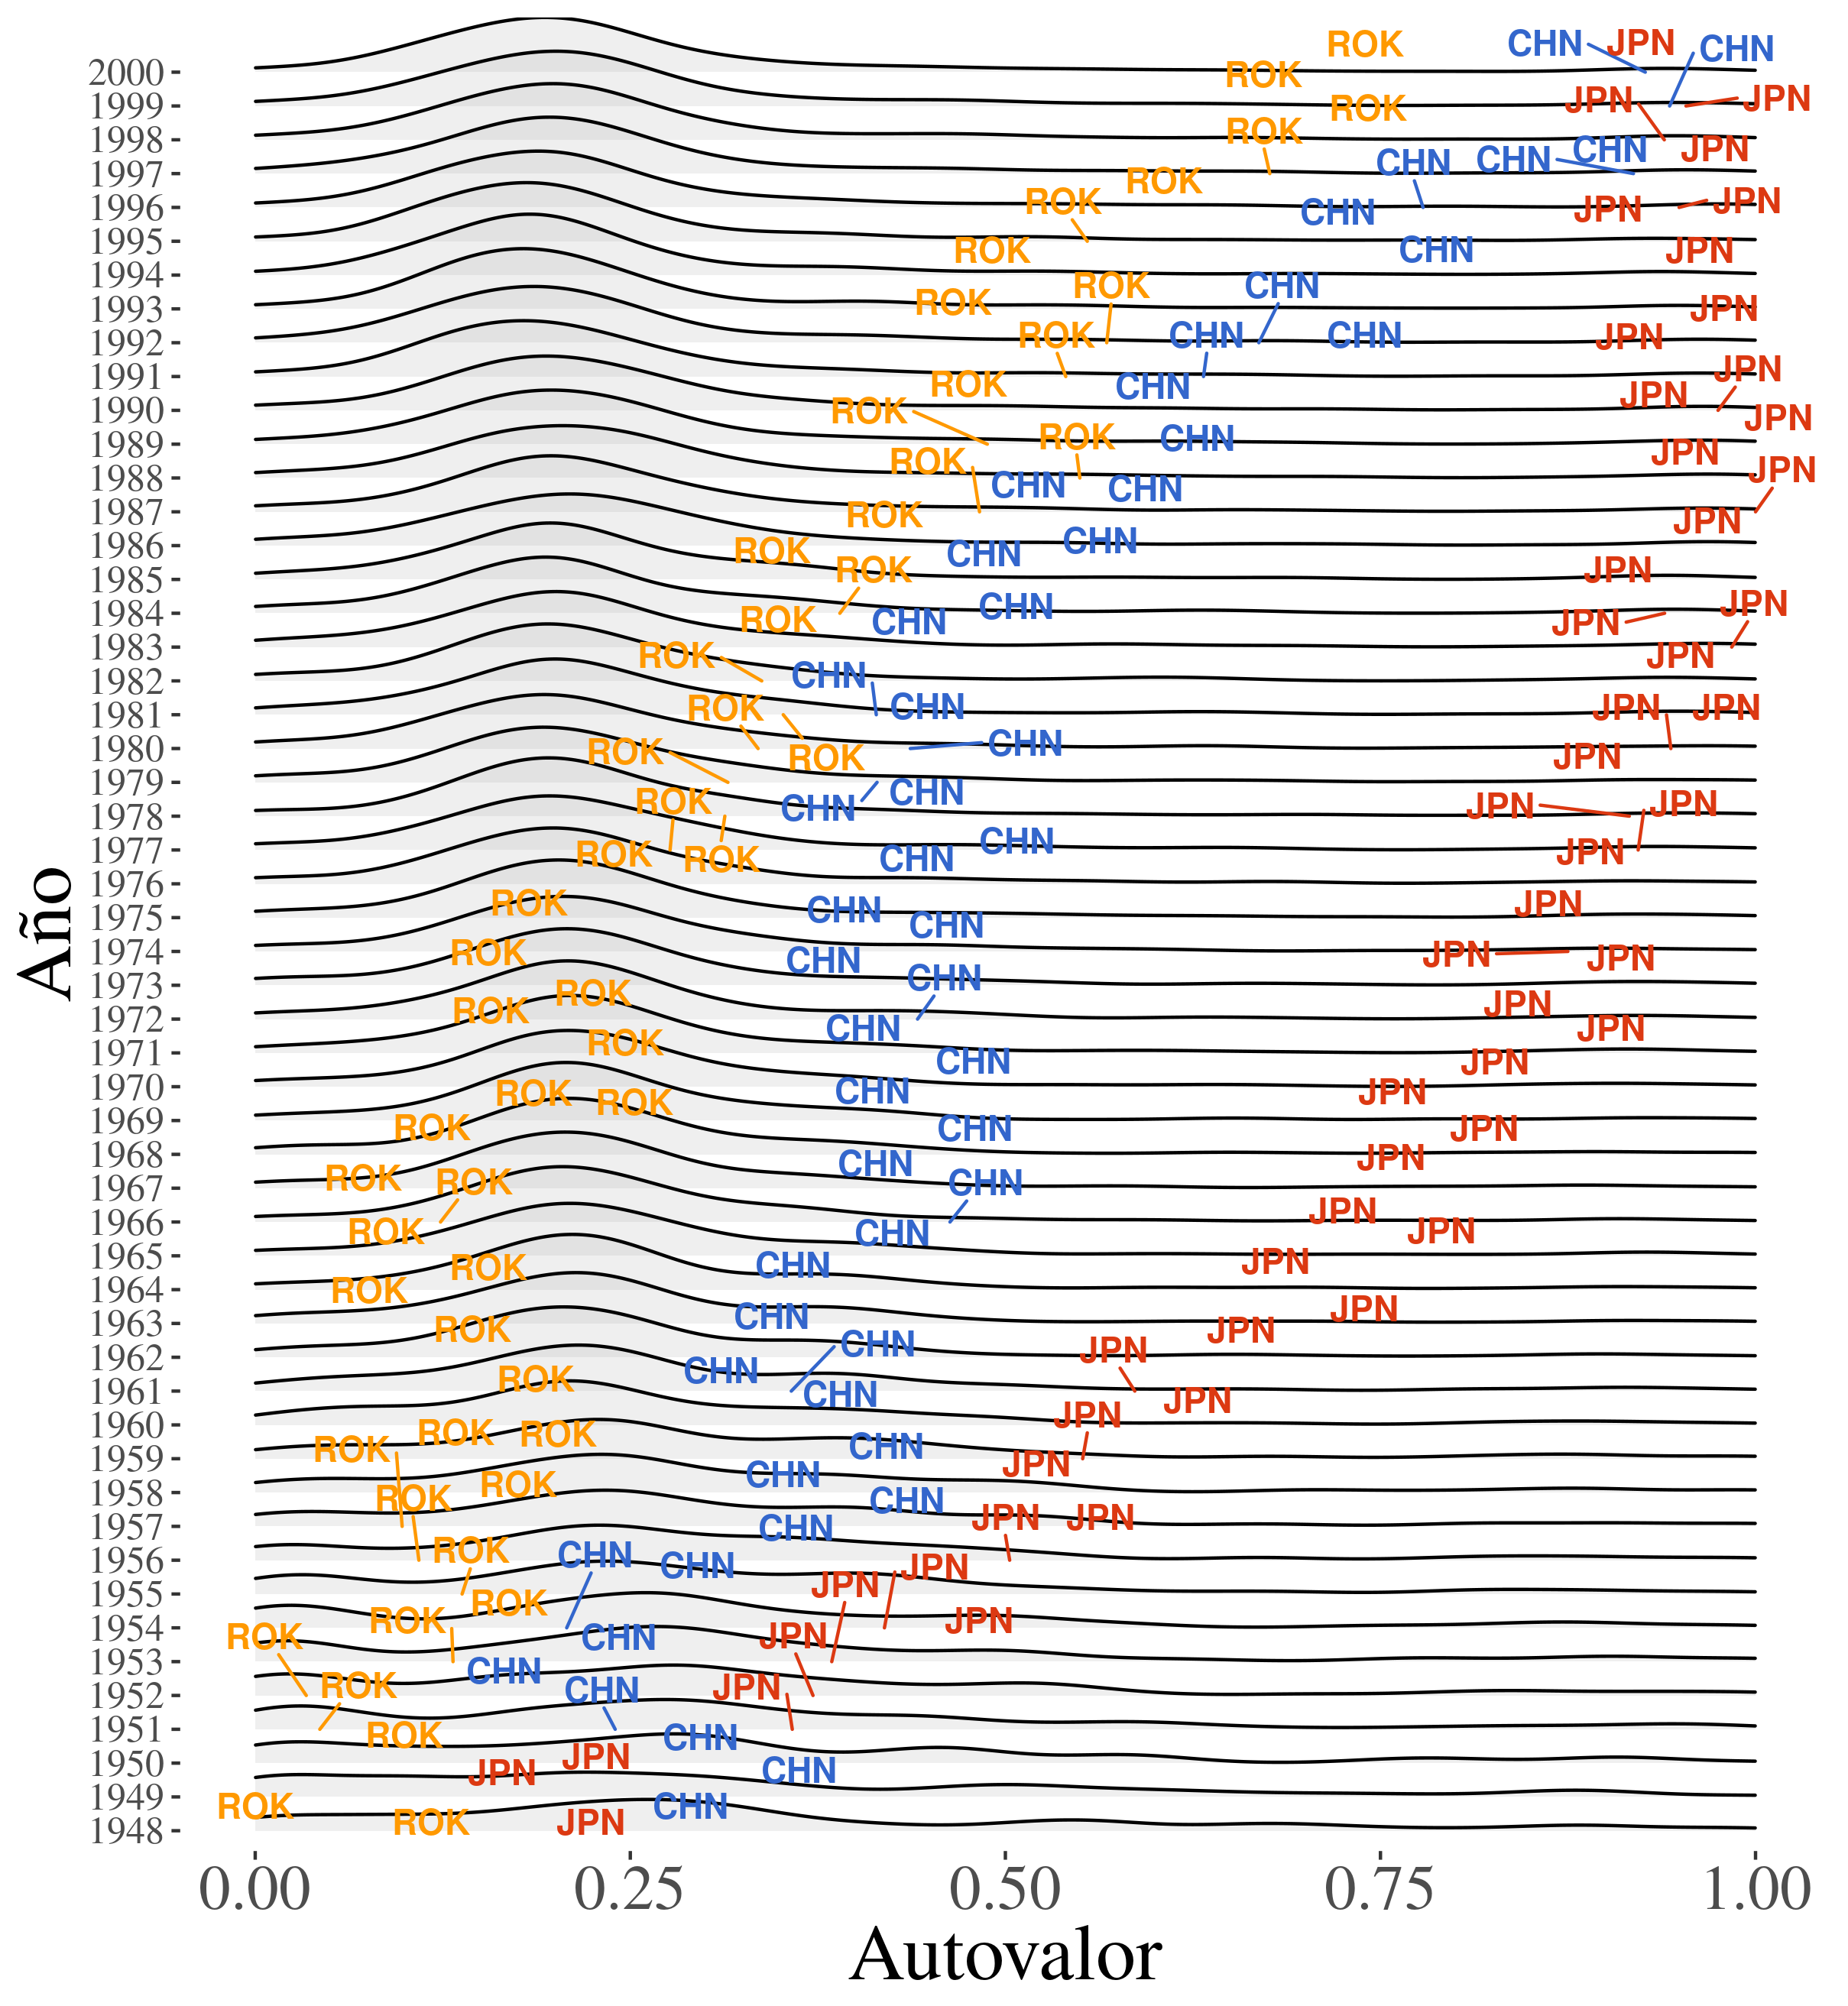
\includegraphics[scale=0.29]{1950_2000_impo_densidad_CHN_JPN_ROK_atvlr}
\end{figure}

\column{.4\textwidth} % Left column and width

\begin{flushleft}
\small
Estos tres países del sudeste asiático tienen una creciente importancia en el comercio mundial a partir de la segunda mitad del S XX, aunque en diferentes momentos. 
\\
\tiny{Más resultados en: \textbf{\url{https://diegokoz.shinyapps.io/Distribucion_nodos_wrdtrade/}}}

\end{flushleft}

\end{columns}
\end{frame}

\section{Comercio a nivel productos}



\begin{frame}
\begin{itemize}[label=\faRebel]
\item Para caracterizar la posición de un país en el mercado mundial, no basta con conocer su importancia relativa.
\item También es necesario entender su rol en términos de la \underline{composición de su canasta exportadora-importadora.}

\end{itemize}
\end{frame}


\begin{frame}

\begin{itemize}[label=\faRebel]
\item Se proponen dos formas distintas de organización de la información:
\item La primera busca las \underline{\textit{dimensiones latentes}} del comercio internacional, basado en \citep{blei2003latent}
\item La segunda se basa en \cite{Hidalgo2007,Hidalgo2009} y proyecta un \textit{espacio de productos} a partir de un \underline{grafo bipartito}, para luego buscar clusters de productos.

\end{itemize}
\end{frame}

\subsection{Topic Modeling}
\subsubsection{Metodología}

\begin{frame}
\centering
\Large Topic Modeling \\

\normalsize Metodología
\end{frame}

\begin{frame}

\begin{columns}[c] 

\column{.45\textwidth} % Right column and width
\begin{figure}
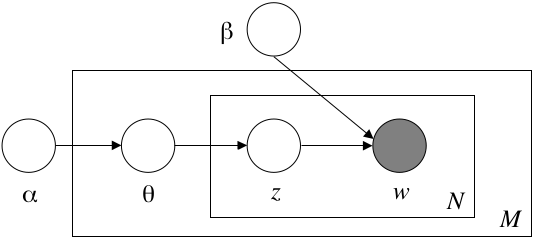
\includegraphics[width=\linewidth]{grafo}

\medskip
\tiny
$\beta \sim Dir_v(\eta)$  Distribución de productos en los componentes latentes\\
$\theta_d \sim Dir_K(\alpha)$ : Distribución de los componentes latentes por país\\
$z_{dn} \sim Mult(\theta_d)$ : Componente latente \\
$w_{dn} \sim Mult(\beta_{zn})$: u\$s comerciado

\end{figure}

\column{.5\textwidth} % Left column and width
\small

\begin{itemize}

\item[\faRebel] Basado en Topic Modeling  \citep{blei2003latent} realizamos inferencia sobre los \textit{componentes latentes} en el comercio internacional utilizando un modelo de inferencia bayesiana
\item[\faRebel] Cómo resultado, obtenemos la \underline{distribución de los productos} sobre los componentes latentes, y la \underline{distribución de los componentes} sobre los países
\end{itemize}

\end{columns}
\end{frame}


\begin{frame}

\begin{itemize}[label=\faRebel]
\item \textbf{Input}: Matriz de dólares exportados por producto para cada país-año (P*Y x N)
\item \textbf{Output}:
\begin{itemize}
\item La distribución de los productos por componente
\item La distribución de los componentes por año-país
\end{itemize}

\item Se construyó una página interactiva para explorar los resultados y asignar etiquetas a los componentes: \textbf{\url{https://treemaps.shinyapps.io/LDA_worldtrade/}}
\item Luego del análisis de componentes, se estudió la evolución de los mismos en la canasta exportadora de los países.

\end{itemize}
\end{frame}


\begin{frame}
\tiny Ejemplo con dos componentes
\begin{figure}
\centering
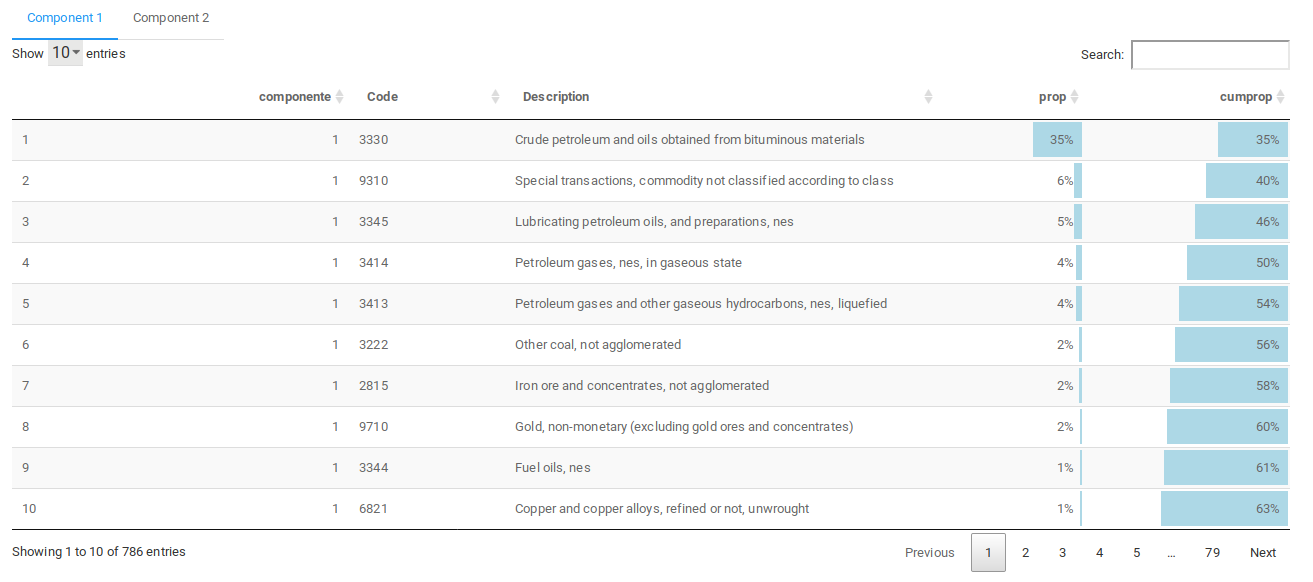
\includegraphics[width=0.8\linewidth]{comp1k2}
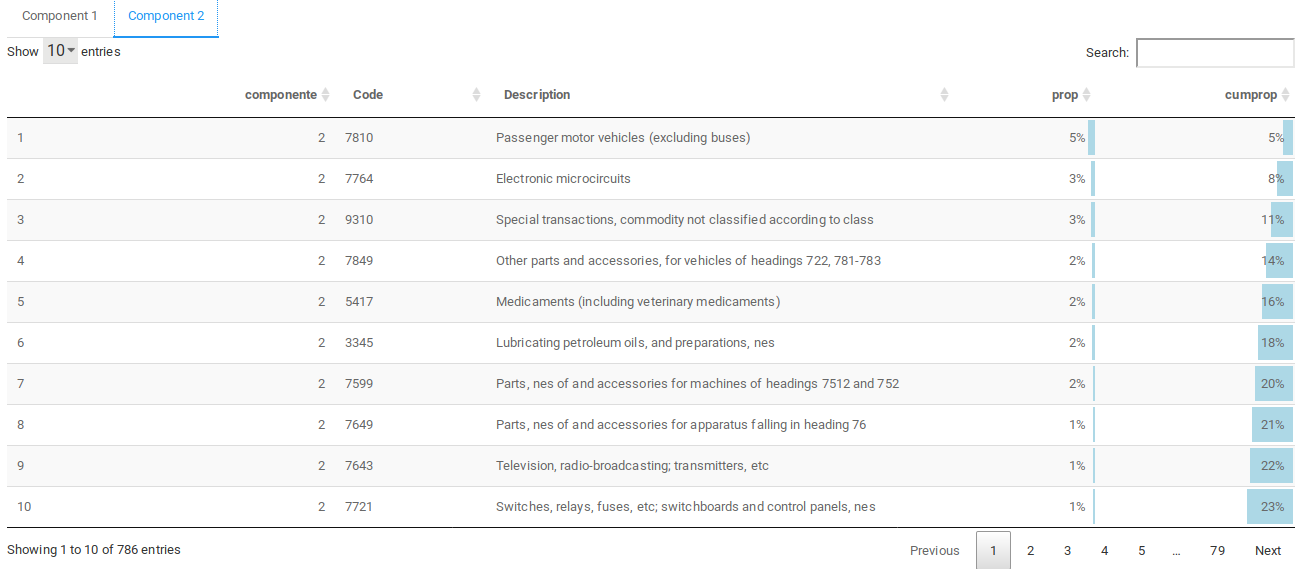
\includegraphics[width=0.8\linewidth]{comp2k2}	
\end{figure}

\end{frame}


\begin{frame}

Para ayudar en la caracterización también se analizó la distribución de cada componente según la clasificación de usos de \cite{lall2000technological}.
\begin{figure}
\centering
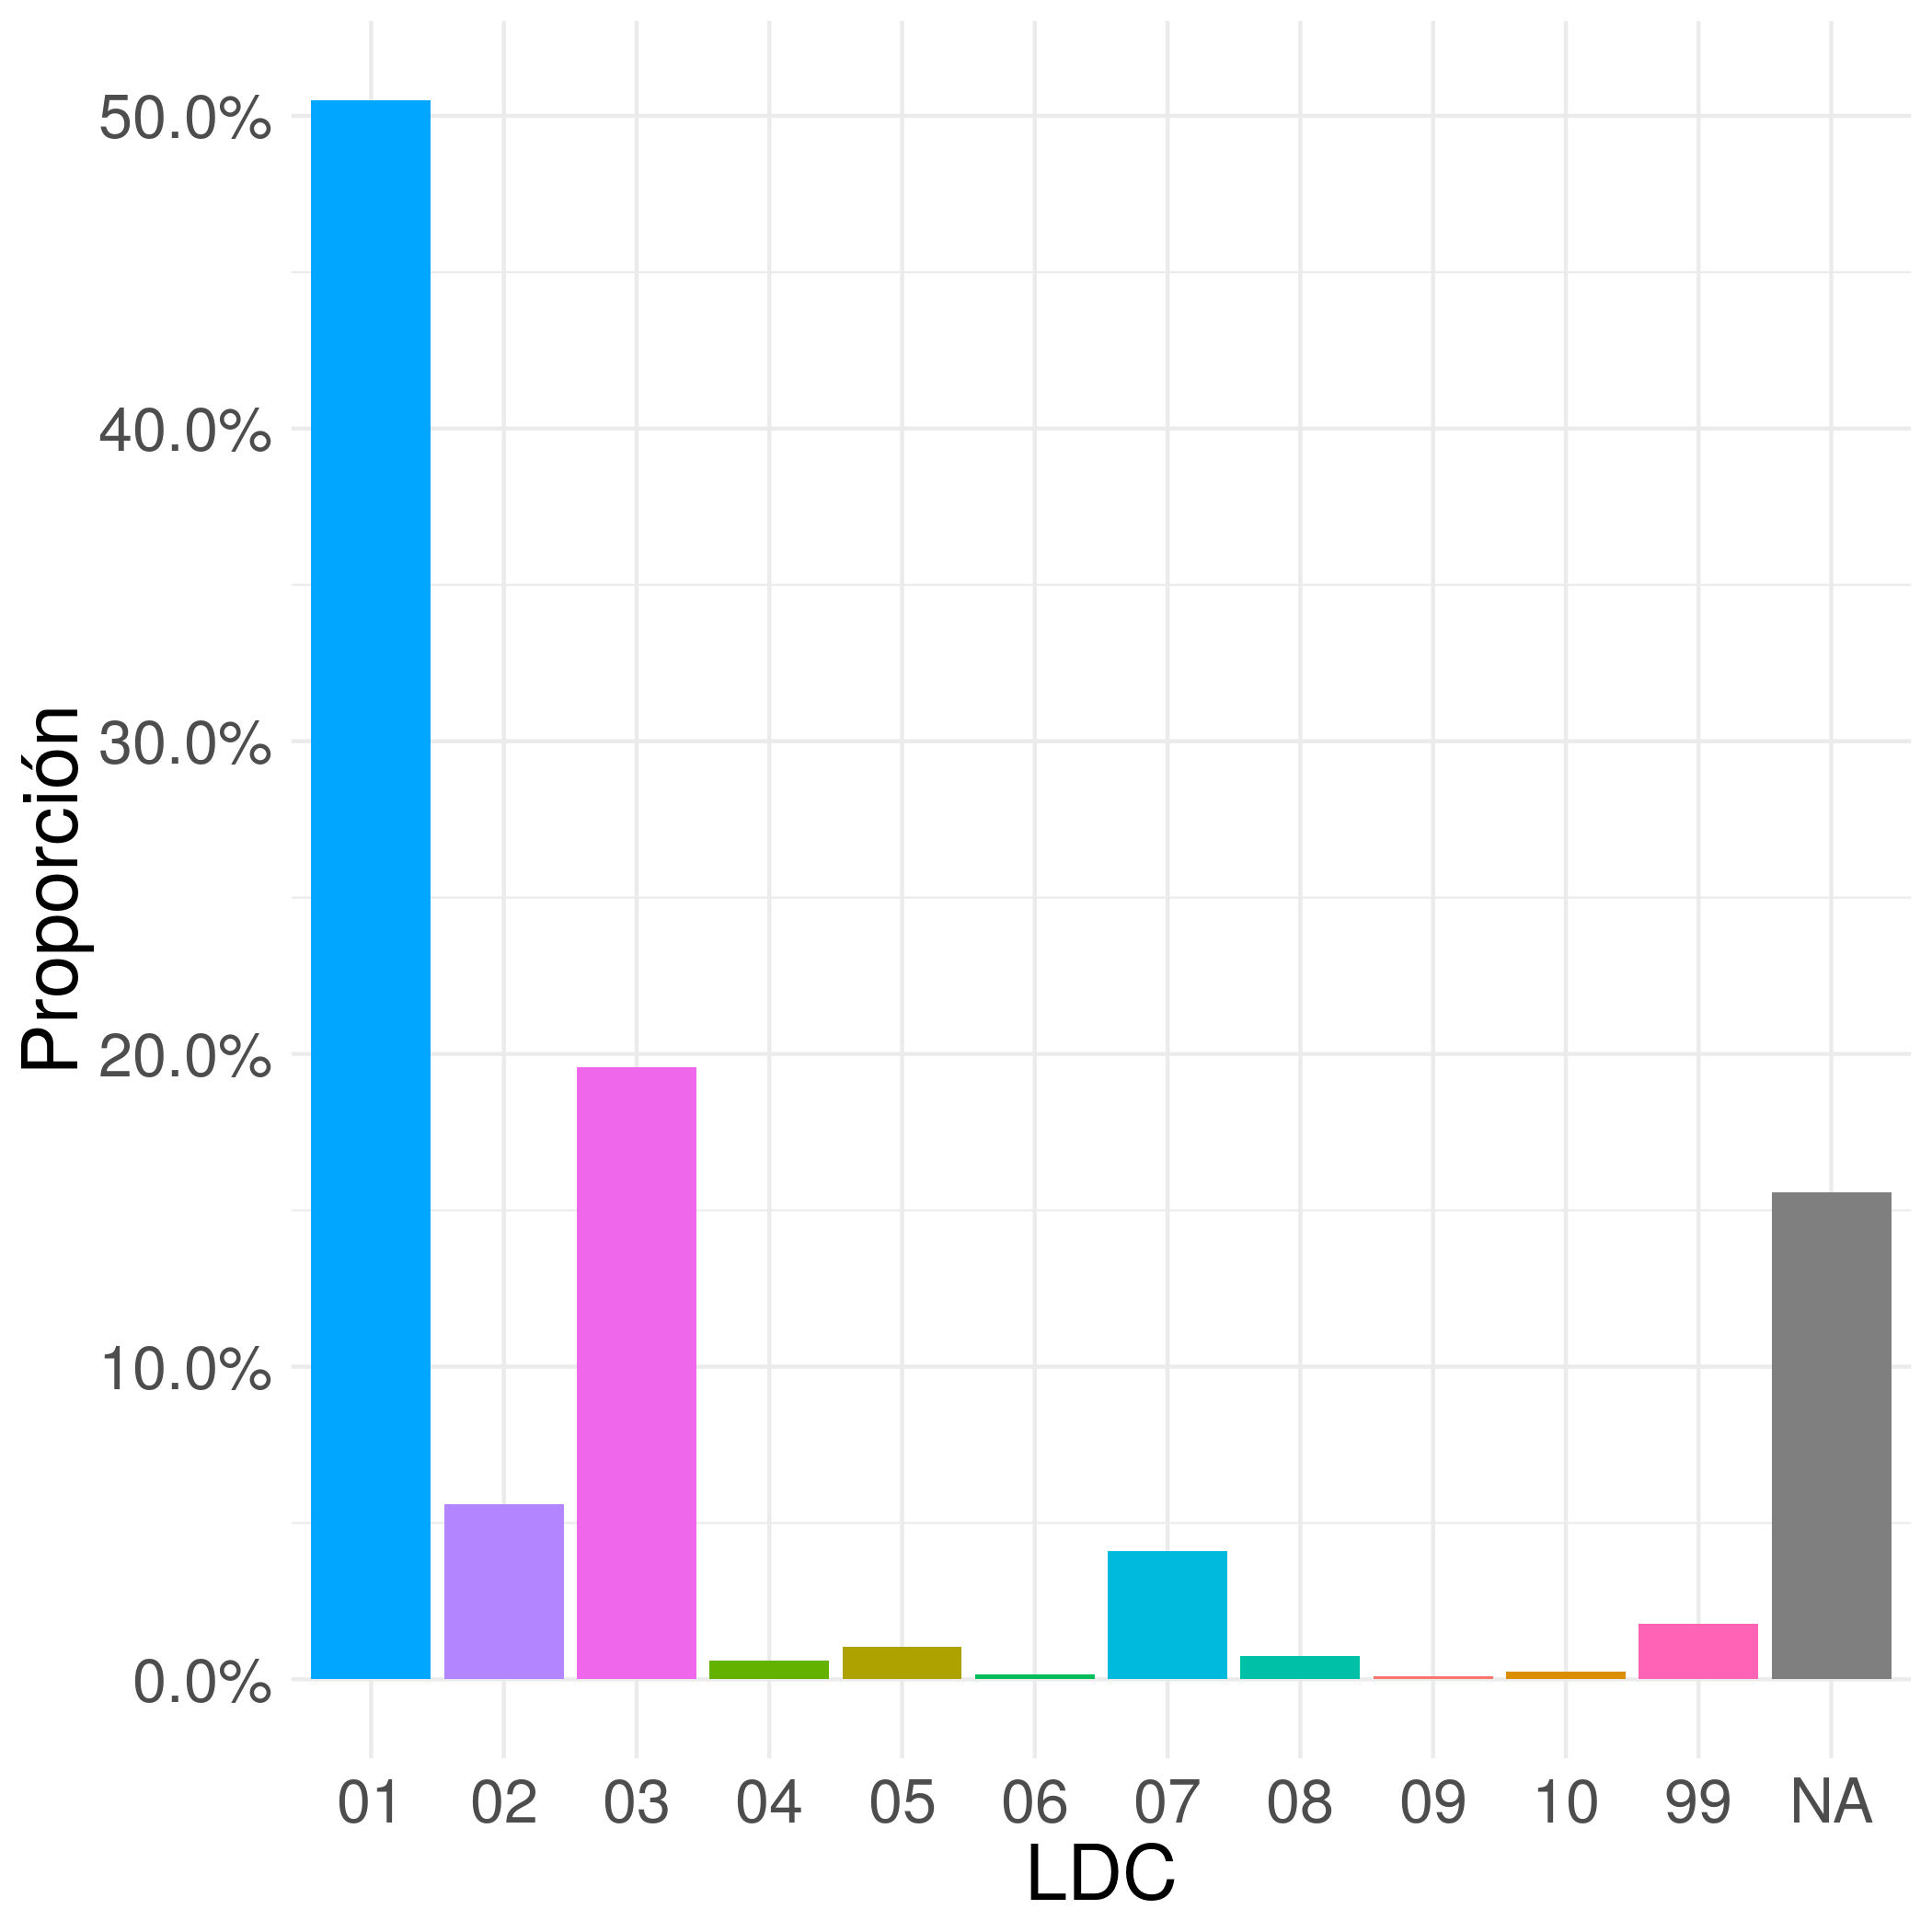
\includegraphics[width=0.45\linewidth]{graficoLall_k2_comp1}
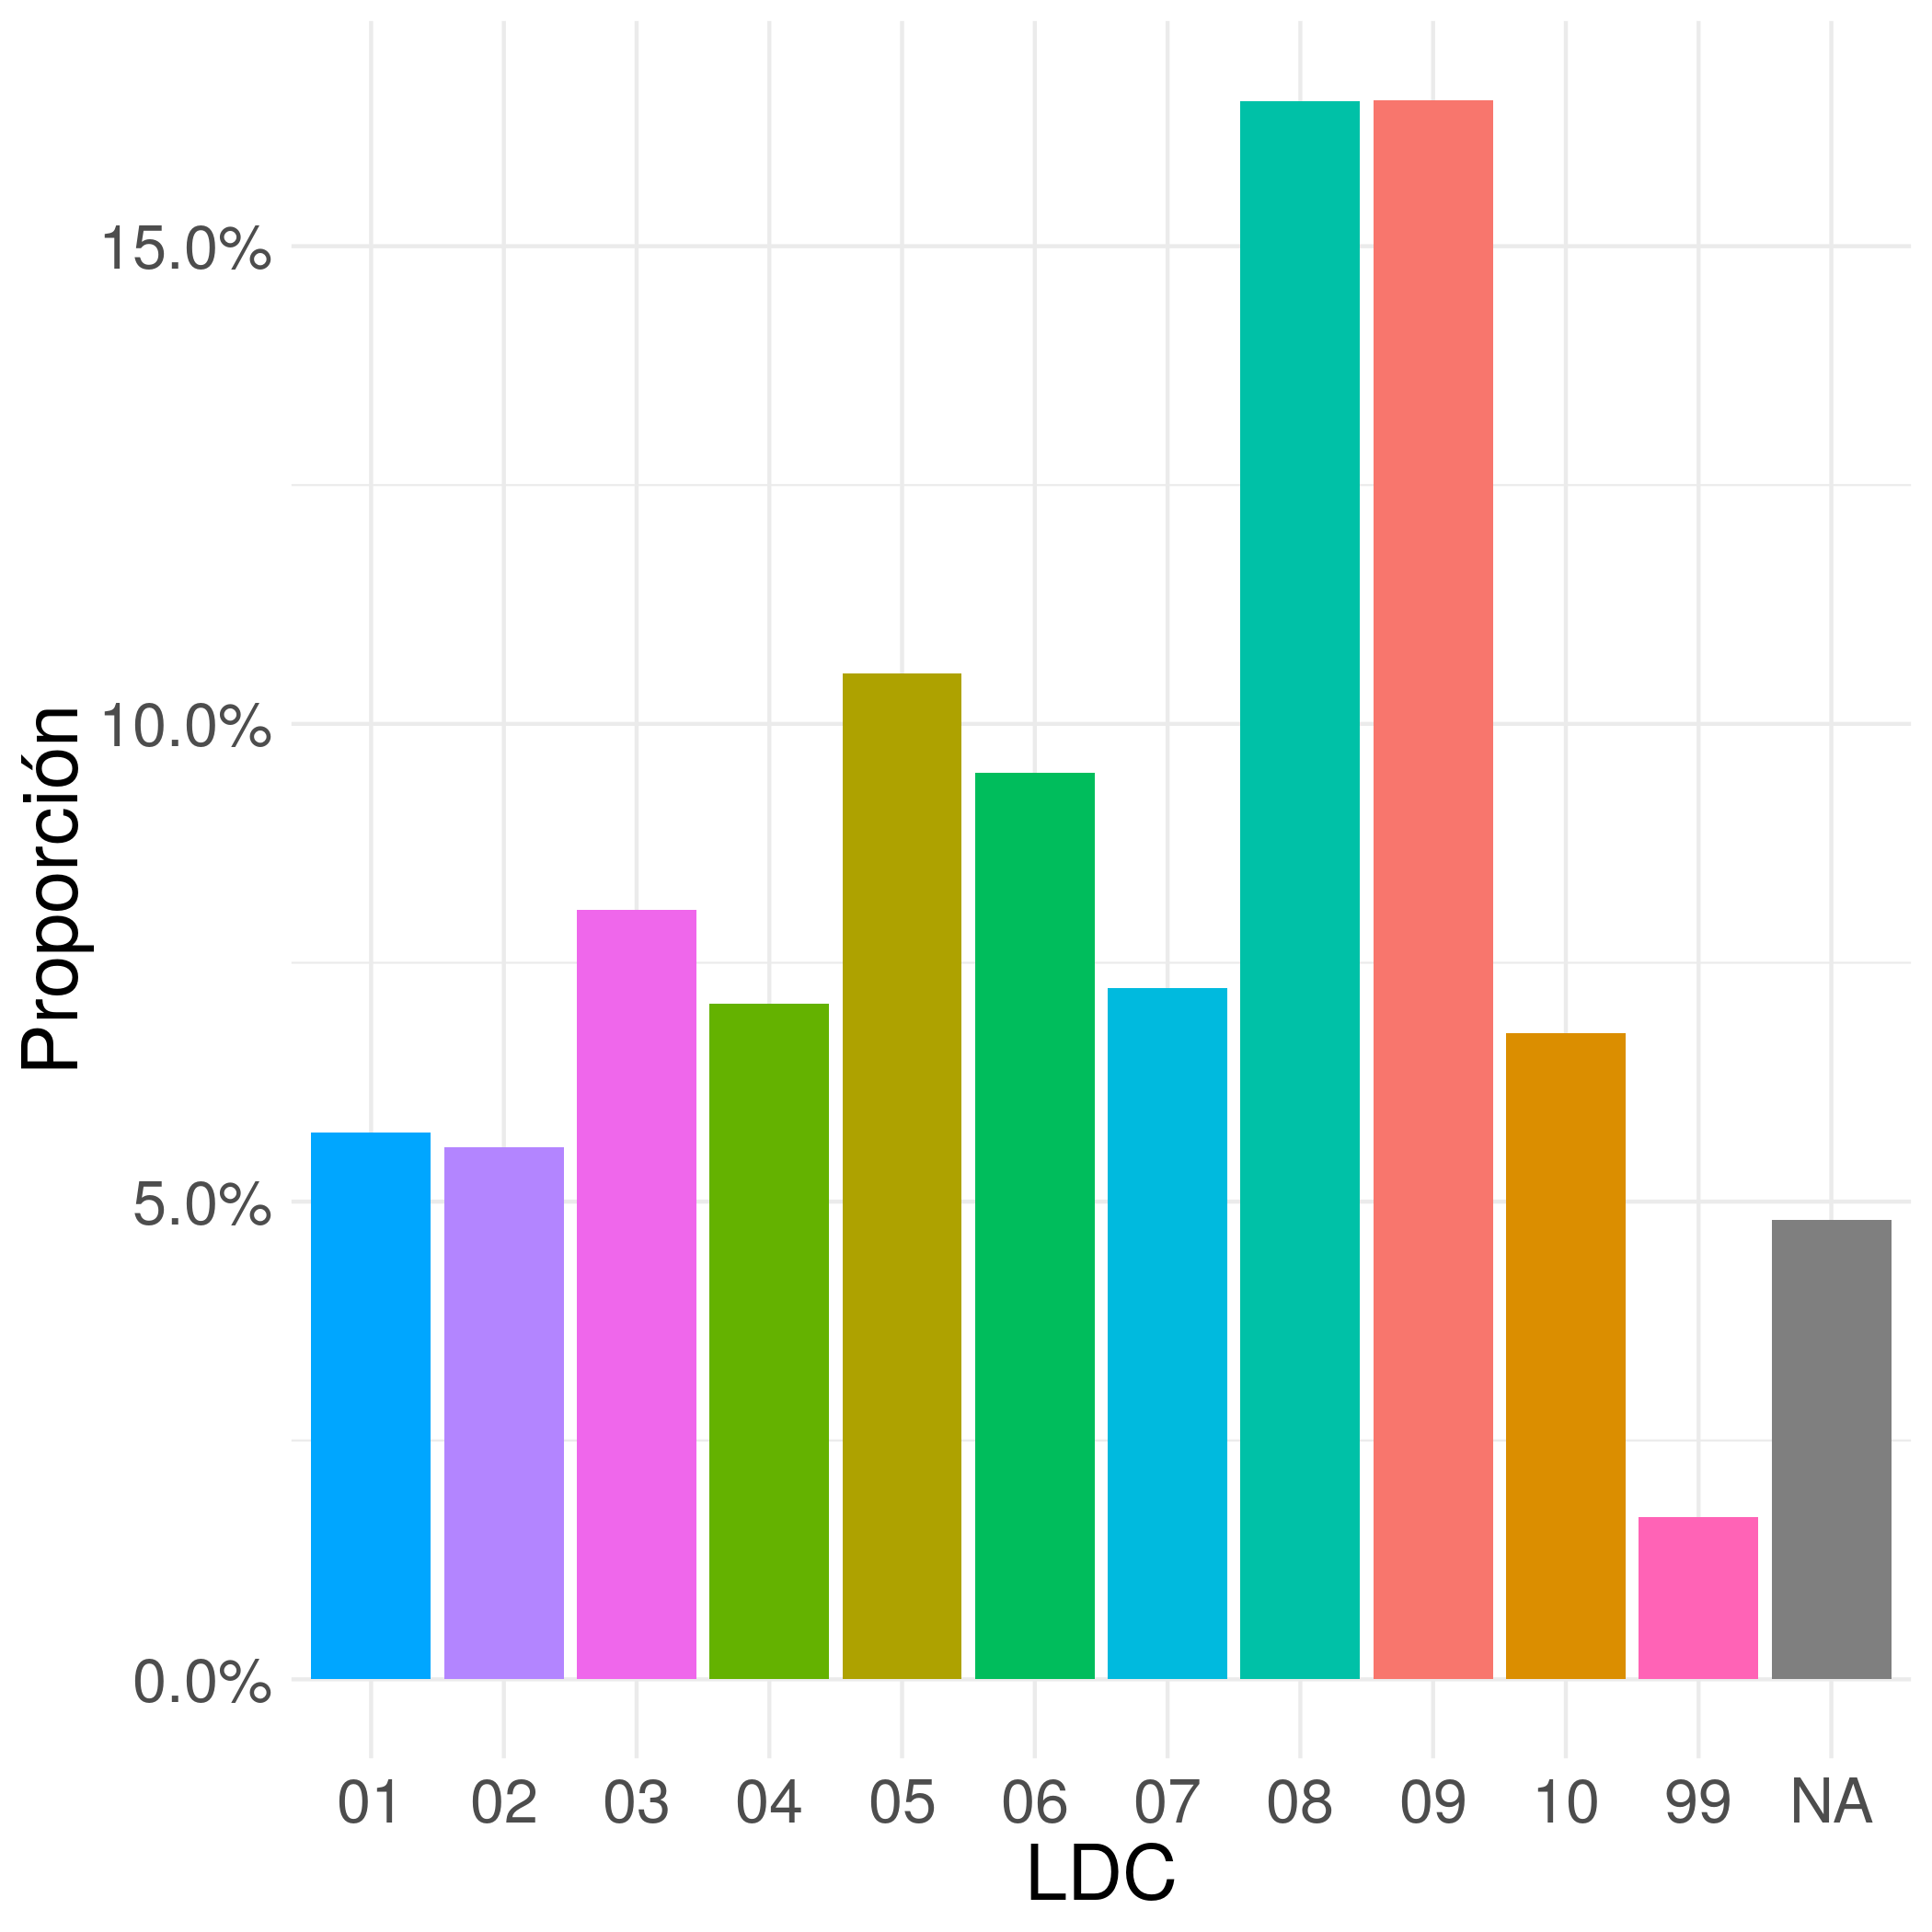
\includegraphics[width=0.45\linewidth]{graficoLall_k2_comp2}	
\end{figure}

De este análisis se concluyó que el mejor número de componentes era 30.

\end{frame}

\subsubsection{Resultados}

\begin{frame}
\centering
\Large Topic Modeling \\

\normalsize Resultados
\end{frame}


\begin{frame}
\small
Caracterización de los componentes según Grupo, subgrupo, Complejidad (industrial) y país característico.
\tiny
\begin{table}
\centering
\begin{tabular}{rllll} 
\hline
\multicolumn{1}{l}{\textbf{Comp}} & \textbf{Grupo}    & \textbf{Subgrupo}                                                                                                                & \textbf{Complejidad} & \textbf{País}                                                      \\ 
\hline
1                                 & Minerales         & Carbón, hierro                                                                                                                   & -                    & Australia                                                          \\ 
\hline
2                                 & Industria         & Textiles, ingenieril, otros                                                                                                      & Baja y media         & San Marino                                                         \\ 
\hline
3                                 & Industria         & Vehículos y partes                                                                                                                      & Media                & Bélgica                                                            \\ 
\hline
4                                 & Industria         & Textiles y juguetes, etc                                                                                                            & Baja                 & Macao                                                              \\ 
\hline
5                                 & Industria         & \begin{tabular}[c]{@{}l@{}}Electrónicos no digitales.\\Cintas de grabación.\\Lineas de telefono.\\Papél fotográfico\end{tabular} & Alta (hasta 70')     & Checoslovaquia                                                     \\ 
\hline
6                                 & Industria         & \begin{tabular}[c]{@{}l@{}}Vehículos, barcos, \\maquinaria y partes\end{tabular}                                                            & Media y alta         & Japón                                                              \\ 
\hline
7                                 & Petróleo          & Estado Gaseoso                                                                                                                   & -                    & Turkmenistán                                                       \\ 
\hline
8                                 & Minerales         & Cobre                                                                                                                            & -                    & Chile                                                              \\ 
\hline
9                                 & Agropecuario      & Café, bananas, otros                                                                                                             & -                    & Réunion                                                            \\ 
\hline
10                                & Industria         & Autos y electrónicos                                                                                                             & Media y alta         & México                                                             \\ 
\hline
11                                & Industria         & \begin{tabular}[c]{@{}l@{}}Autos, partes y\\ componentes\end{tabular}                                                            & Media         & Alemania                                                           \\ 
\hline
12                                & Petróleo          & Crudo                                                                                                                            & -                    & Sudán del Sur                                                      \\ 
\hline
13                                & -                 & Oro, relojes, joyas                                                                                                              & -                    & Suiza                                                              \\ 
\hline
14                                & Industria         & Químicos                                                                                                                         & -                 & Curazao                                                            \\ 
\hline
15                                & Minerales         & Diamantes                                                                                                                        & -                    & Botswana                                                           \\ 
\hline
16                                & Industria + Agro. & \begin{tabular}[c]{@{}l@{}}Aviones, autopartes,\\ soja y maíz\end{tabular}                                                       & Media y alta         & USA                                                                \\ 
\hline

\end{tabular}
\end{table}

\begin{flushright}
1/2
\end{flushright}
\end{frame}

\begin{frame}
\tiny
\begin{table}
\centering
\begin{tabular}{rllll} 
\hline
\multicolumn{1}{l}{\textbf{Comp}} & \textbf{Grupo}    & \textbf{Subgrupo}                                                                                                                & \textbf{Complejidad} & \textbf{País}                                                      \\ 
\hline
17                                & Industria + Agro. & \begin{tabular}[c]{@{}l@{}}Autopartes,\\ madera y derivados\end{tabular}                                                         & Media                & Finlandia                                                          \\ 
\hline
18                                & Industria + Agro. & \begin{tabular}[c]{@{}l@{}}Productos primarios\\ y textiles\end{tabular}                                                         & Baja                 & Isla de Navidad                                                    \\ 
\hline
19                                & -                 & \begin{tabular}[c]{@{}l@{}}Transacciones especiales,\\ no clasificadas\end{tabular}                                              & -                    & Isla San Martín                                                    \\ 
\hline
20                                & Combustibles      & Fuel oil, gasolina, etc.                                                                                                         & -                    & \begin{tabular}[c]{@{}l@{}}Rep. Dem.\\ Pop.del Yemen\end{tabular}  \\ 
\hline
21                                & Industria         & \begin{tabular}[c]{@{}l@{}}Medicamentos e\\ instrumentos médicos.\end{tabular}                                                   & Alta                 & Irlanda                                                            \\ 
\hline
22                                & Petróleo + Agro   & \begin{tabular}[c]{@{}l@{}}Hidrocarburos,\\aceite de palma,cacao, etc.\end{tabular}                                              & -                    & Ghana                                                              \\ 
\hline
23                                & Industria         & \begin{tabular}[c]{@{}l@{}}Procesadores,\\microcircuitos,\\ juguetes y calzado.\end{tabular}                                     & Alta y baja          & China                                                              \\ 
\hline
24                                & Industra + Agro.      & \begin{tabular}[c]{@{}l@{}}Barcos, carnes, pescados,\\ lácteos\end{tabular}                                                              & Media                    & Islandia                                                           \\ 
\hline
25                                & Minerales + Agro. & Soja y derivados, Hierro                                                                                                                    & -                    & Paraguay                                                           \\ 
\hline
26                                & Industria + Agro. & \begin{tabular}[c]{@{}l@{}}Aviones, perfumería,\\ vino \end{tabular}                                                       & Alta                 & Francia                                                            \\ 
\hline
27                                & Industria         & Microcircuitos                                                                                                                   & Alta                 & filipinas                                                          \\ 
\hline
28                                & Industria + Agro. & \begin{tabular}[c]{@{}l@{}}Arroz, algodón,\\textiles, goma, etc.\end{tabular}                                                 & Baja                 & Pakistán                                                           \\ 
\hline
29                                & Industria + Agro. & maquinaria, flores, quesos.                                                                                                      & Alta                 & Países Bajos                                                       \\ 
\hline
30                                & Industria         & \begin{tabular}[c]{@{}l@{}}Vehículos, partes \\y medicamentos \end{tabular} & Media y alta         & Reino Unido                                                        \\
\hline
\end{tabular}
\end{table}
\begin{flushright}
2/2
\end{flushright}
\end{frame}


\begin{frame}

\small

Distribución de componentes en países I. Países petroleros.

\begin{columns}[c] 

\column{.6\textwidth} % Right column and width
\begin{figure}
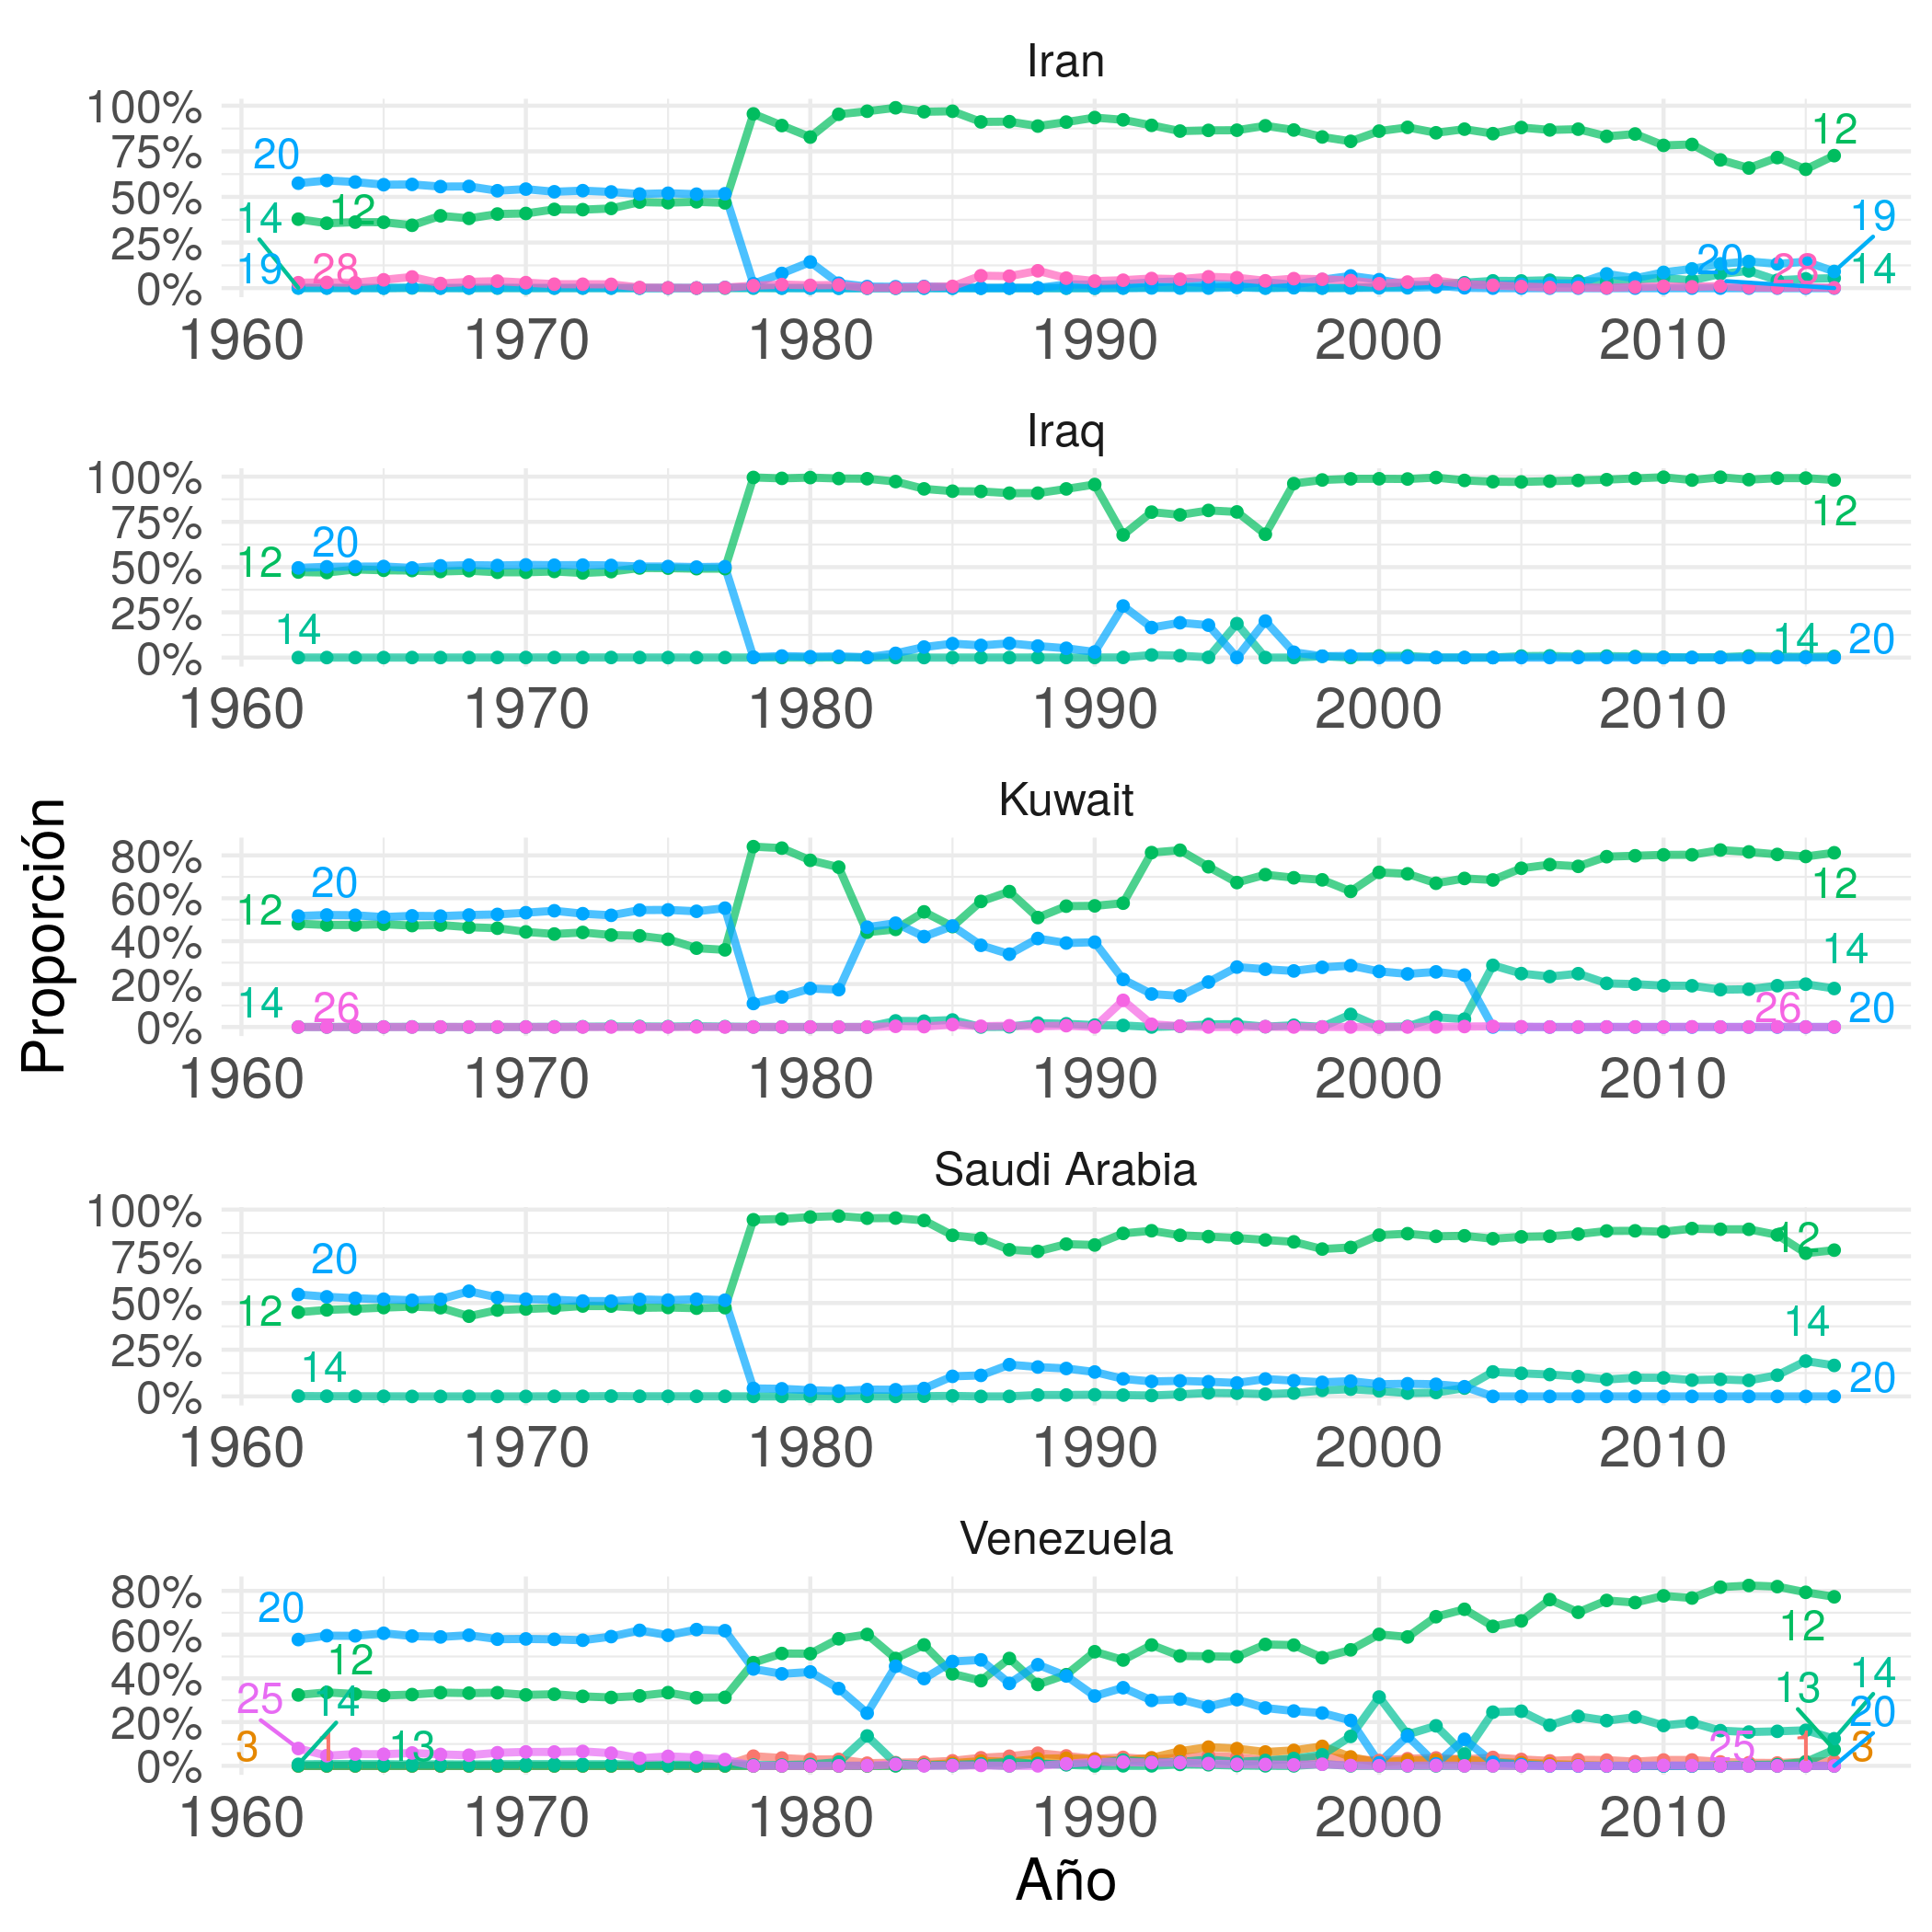
\includegraphics[width=\linewidth]{graficoLDA_k30_IRN_IRQ_KWT_SAU_VEN}
\end{figure}

\column{.4\textwidth} % Left column and width

A partir de la crisis del petróleo del 70' \underline{reprimarizan su producción} y pasan de derivados del petroleo, \textit{Fuel Oil}, a Petróleo crudo.

\end{columns} 

\end{frame}


\begin{frame}
\small
Distribución de componentes en países II. Canadá, México y Estados Unidos
\scriptsize
\begin{columns}[c] 

\column{.55\textwidth} % Right column and width
\begin{figure}
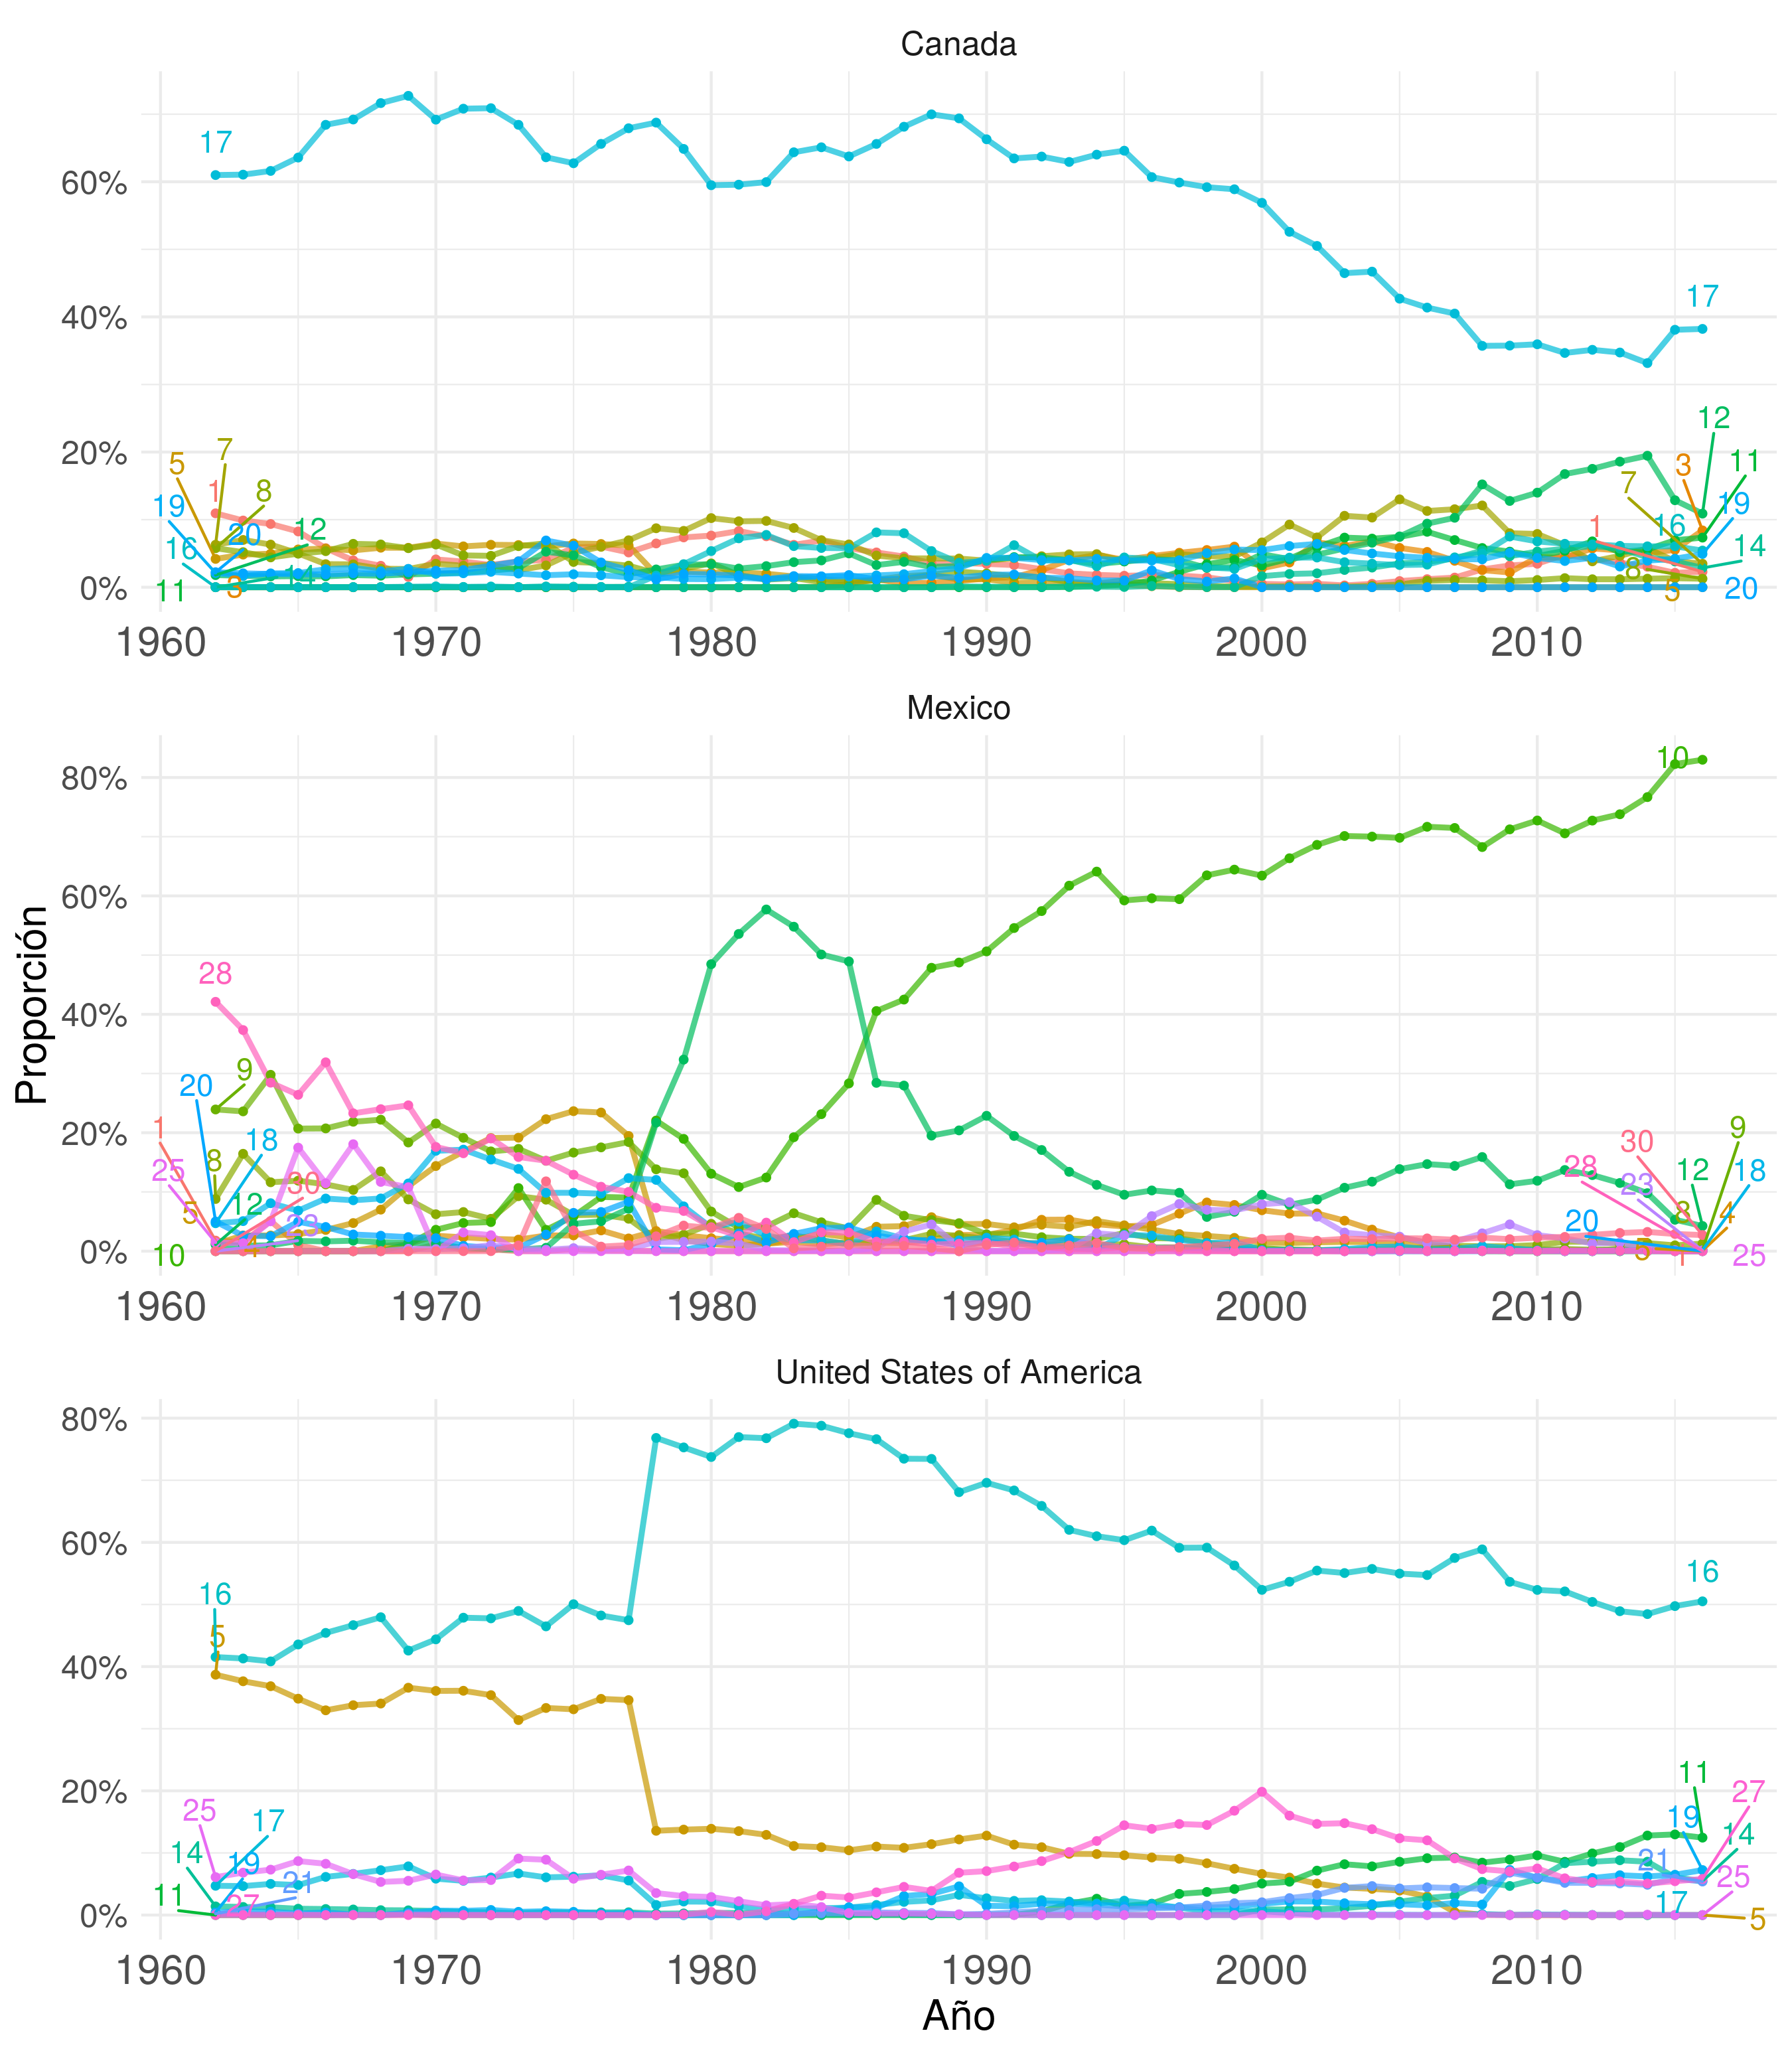
\includegraphics[width=\linewidth]{graficoLDA_k30_CAN_MEX_USA}
\end{figure}

\column{.6\textwidth} % Left column and width

\begin{itemize}[label=\faRebel]
\item En \underline{Canadá} domina el componente 17: \underline{Industria más producción maderera} y derivados. Sin embargo, desde mediados de los 90' crecen en importancia el \underline{petróleo} y derivados (comp. 12 y 7)
\item En \underline{México} se observa un \underline{boom petrolero} entre mediados de los 70' hasta mediados de los 80'. A partir de allí se observa el fenómeno conocido como la \underline{\textit{Maquila mexicana}}.
\item \underline{Estados Unidos} exporta en el componente 5, de alta tecnología\underline{ hasta los 70'}. Luego toma su lugar el componente 16: aviones y autopartes, pero también maíz y soja
\end{itemize}

\end{columns} 

\end{frame}


\begin{frame}
\small
Distribución de componentes en países III. Argentina, Brasil y Uruguay
\scriptsize
\begin{columns}[c] 

\column{.55\textwidth} % Right column and width
\begin{figure}
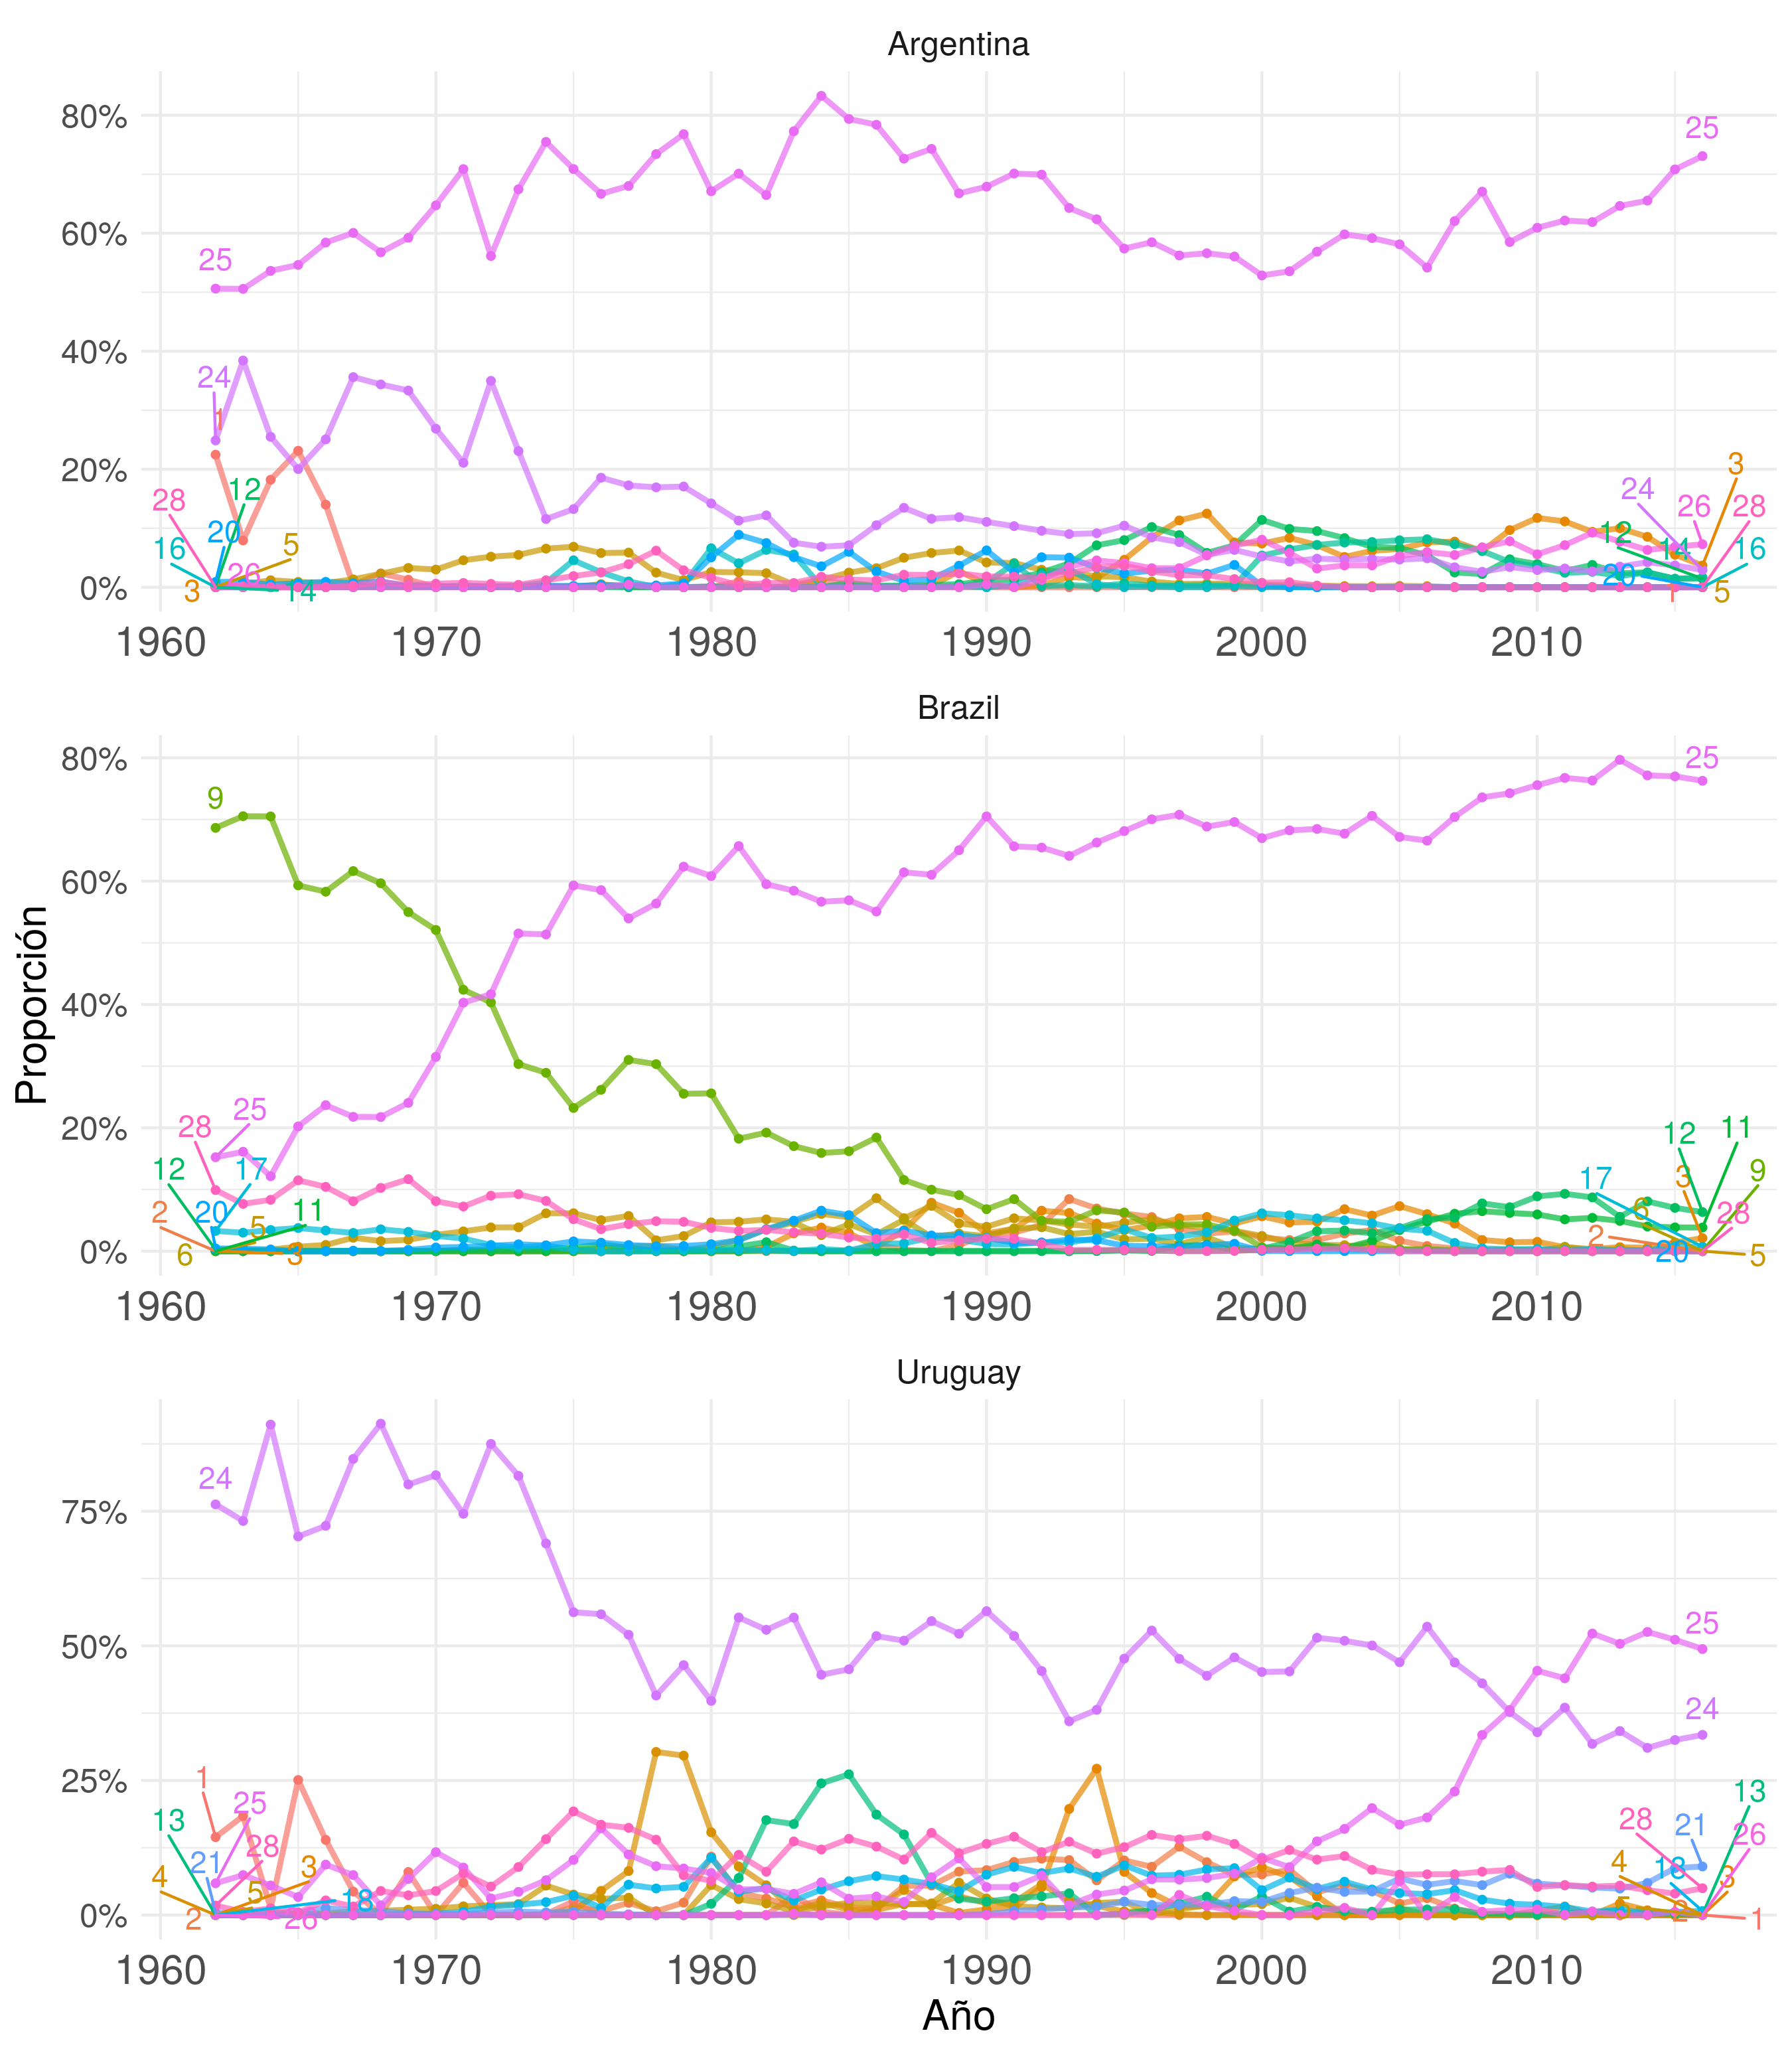
\includegraphics[width=\linewidth]{graficoLDA_k30_ARG_BRA_URY}
\end{figure}

\column{.6\textwidth} % Left column and width

\begin{itemize}[label=\faRebel]
\item En los tres países el componente más importante al finalizar la serie es el 25 (\underline{soja}).
\item En \underline{Argentina} al principio de la serie tiene importancia el comp. 24 (Ganadería). En \underline{Uruguay} ese componente es el más importante hasta casi el final de la serie.
\item En \underline{Brasil} La producción sojera reemplaza al componente 9(café, bananas,etc.), dominante en los 60' y 70'.
\end{itemize}

\end{columns} 

\end{frame}


\begin{frame}
\small
Distribución de componentes en países IV. Francia, Irlanda y Reino Unido
\scriptsize
\begin{columns}[c] 

\column{.55\textwidth} % Right column and width
\begin{figure}
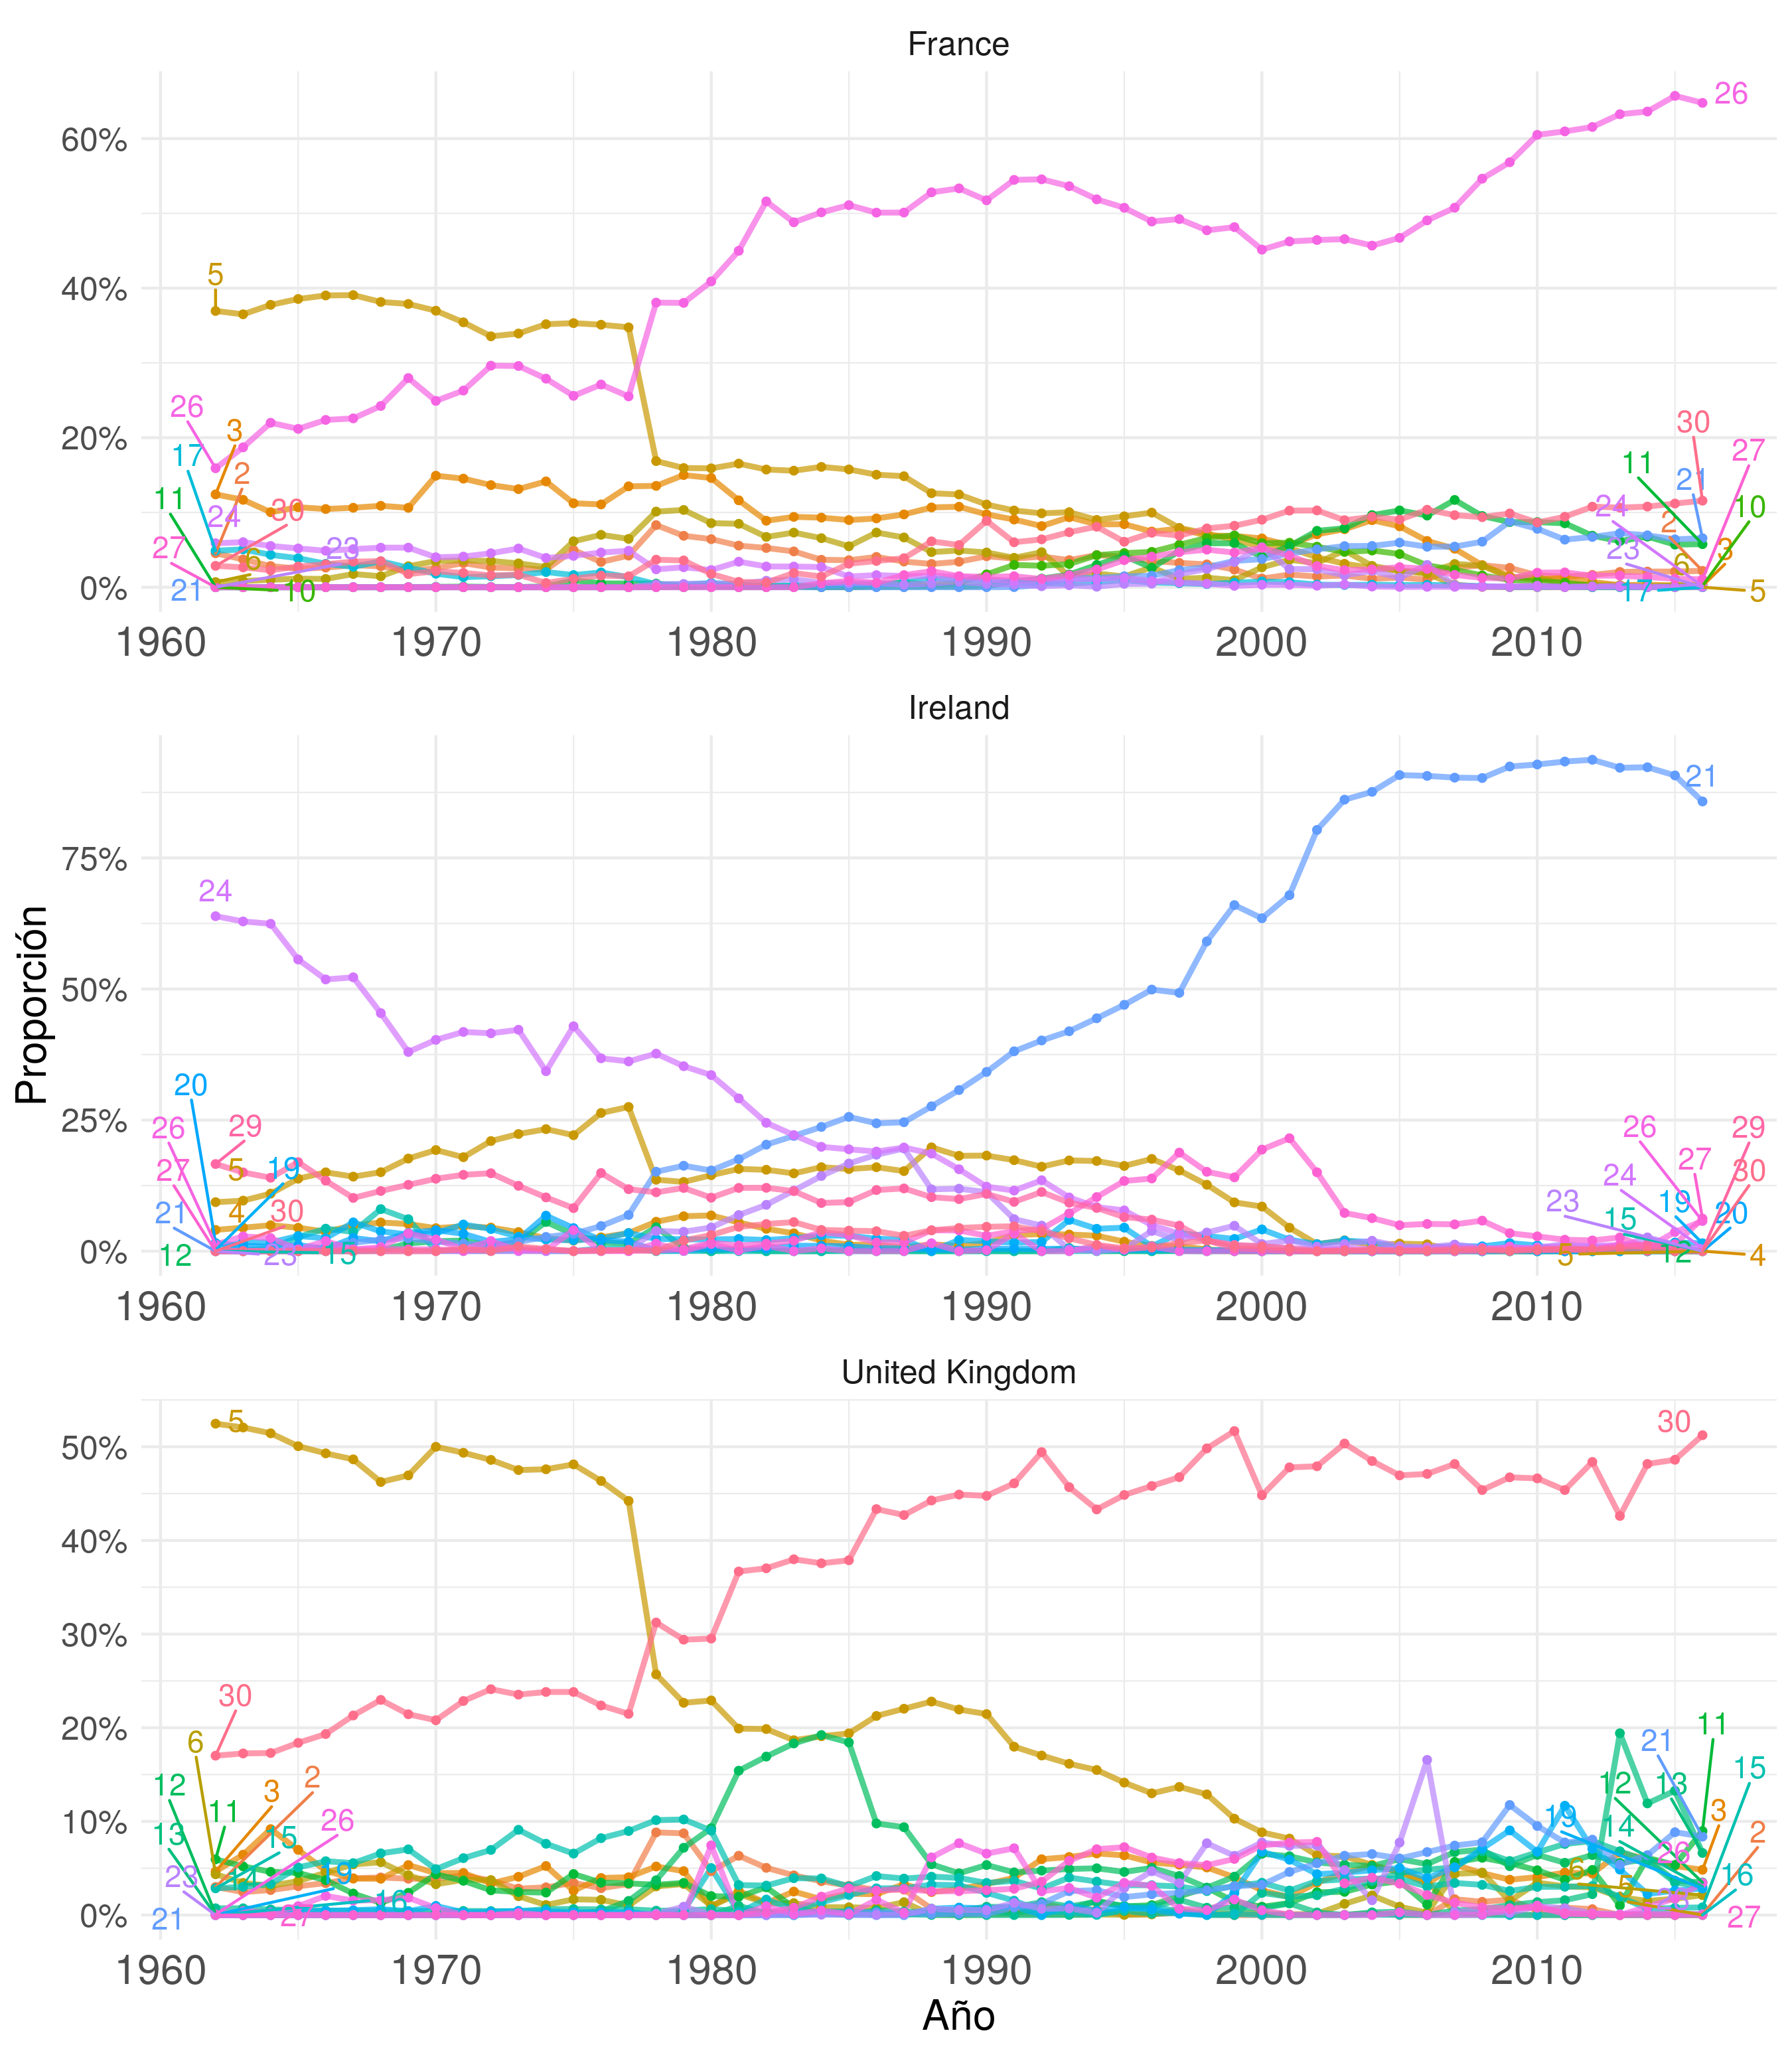
\includegraphics[width=\linewidth]{graficoLDA_k30_FRA_GBR_IRL}
\end{figure}

\column{.6\textwidth} % Left column and width

\begin{itemize}[label=\faRebel]
\item Francia y Reino Unido también exportaban sobre el comp. 5 hasta fines de los 70' y luego pasan a un componente característico.
\item \underline{Francia} exporta en el comp. 26 (\underline{Aviones, perfumería y vino}) y \underline{UK} en el 30(\underline{Vehículos, partes y medicamentos}).
\item A mediados de los 80' \underline{Irlanda} pasa del comp.24 (ganadería) al 21, de industria de alta complejidad.
\end{itemize}

\end{columns} 

\end{frame}


\begin{frame}
\small
Distribución de componentes en países IV. China, Japón y Filipinas
\scriptsize
\begin{columns}[c] 

\column{.55\textwidth} % Right column and width
\begin{figure}
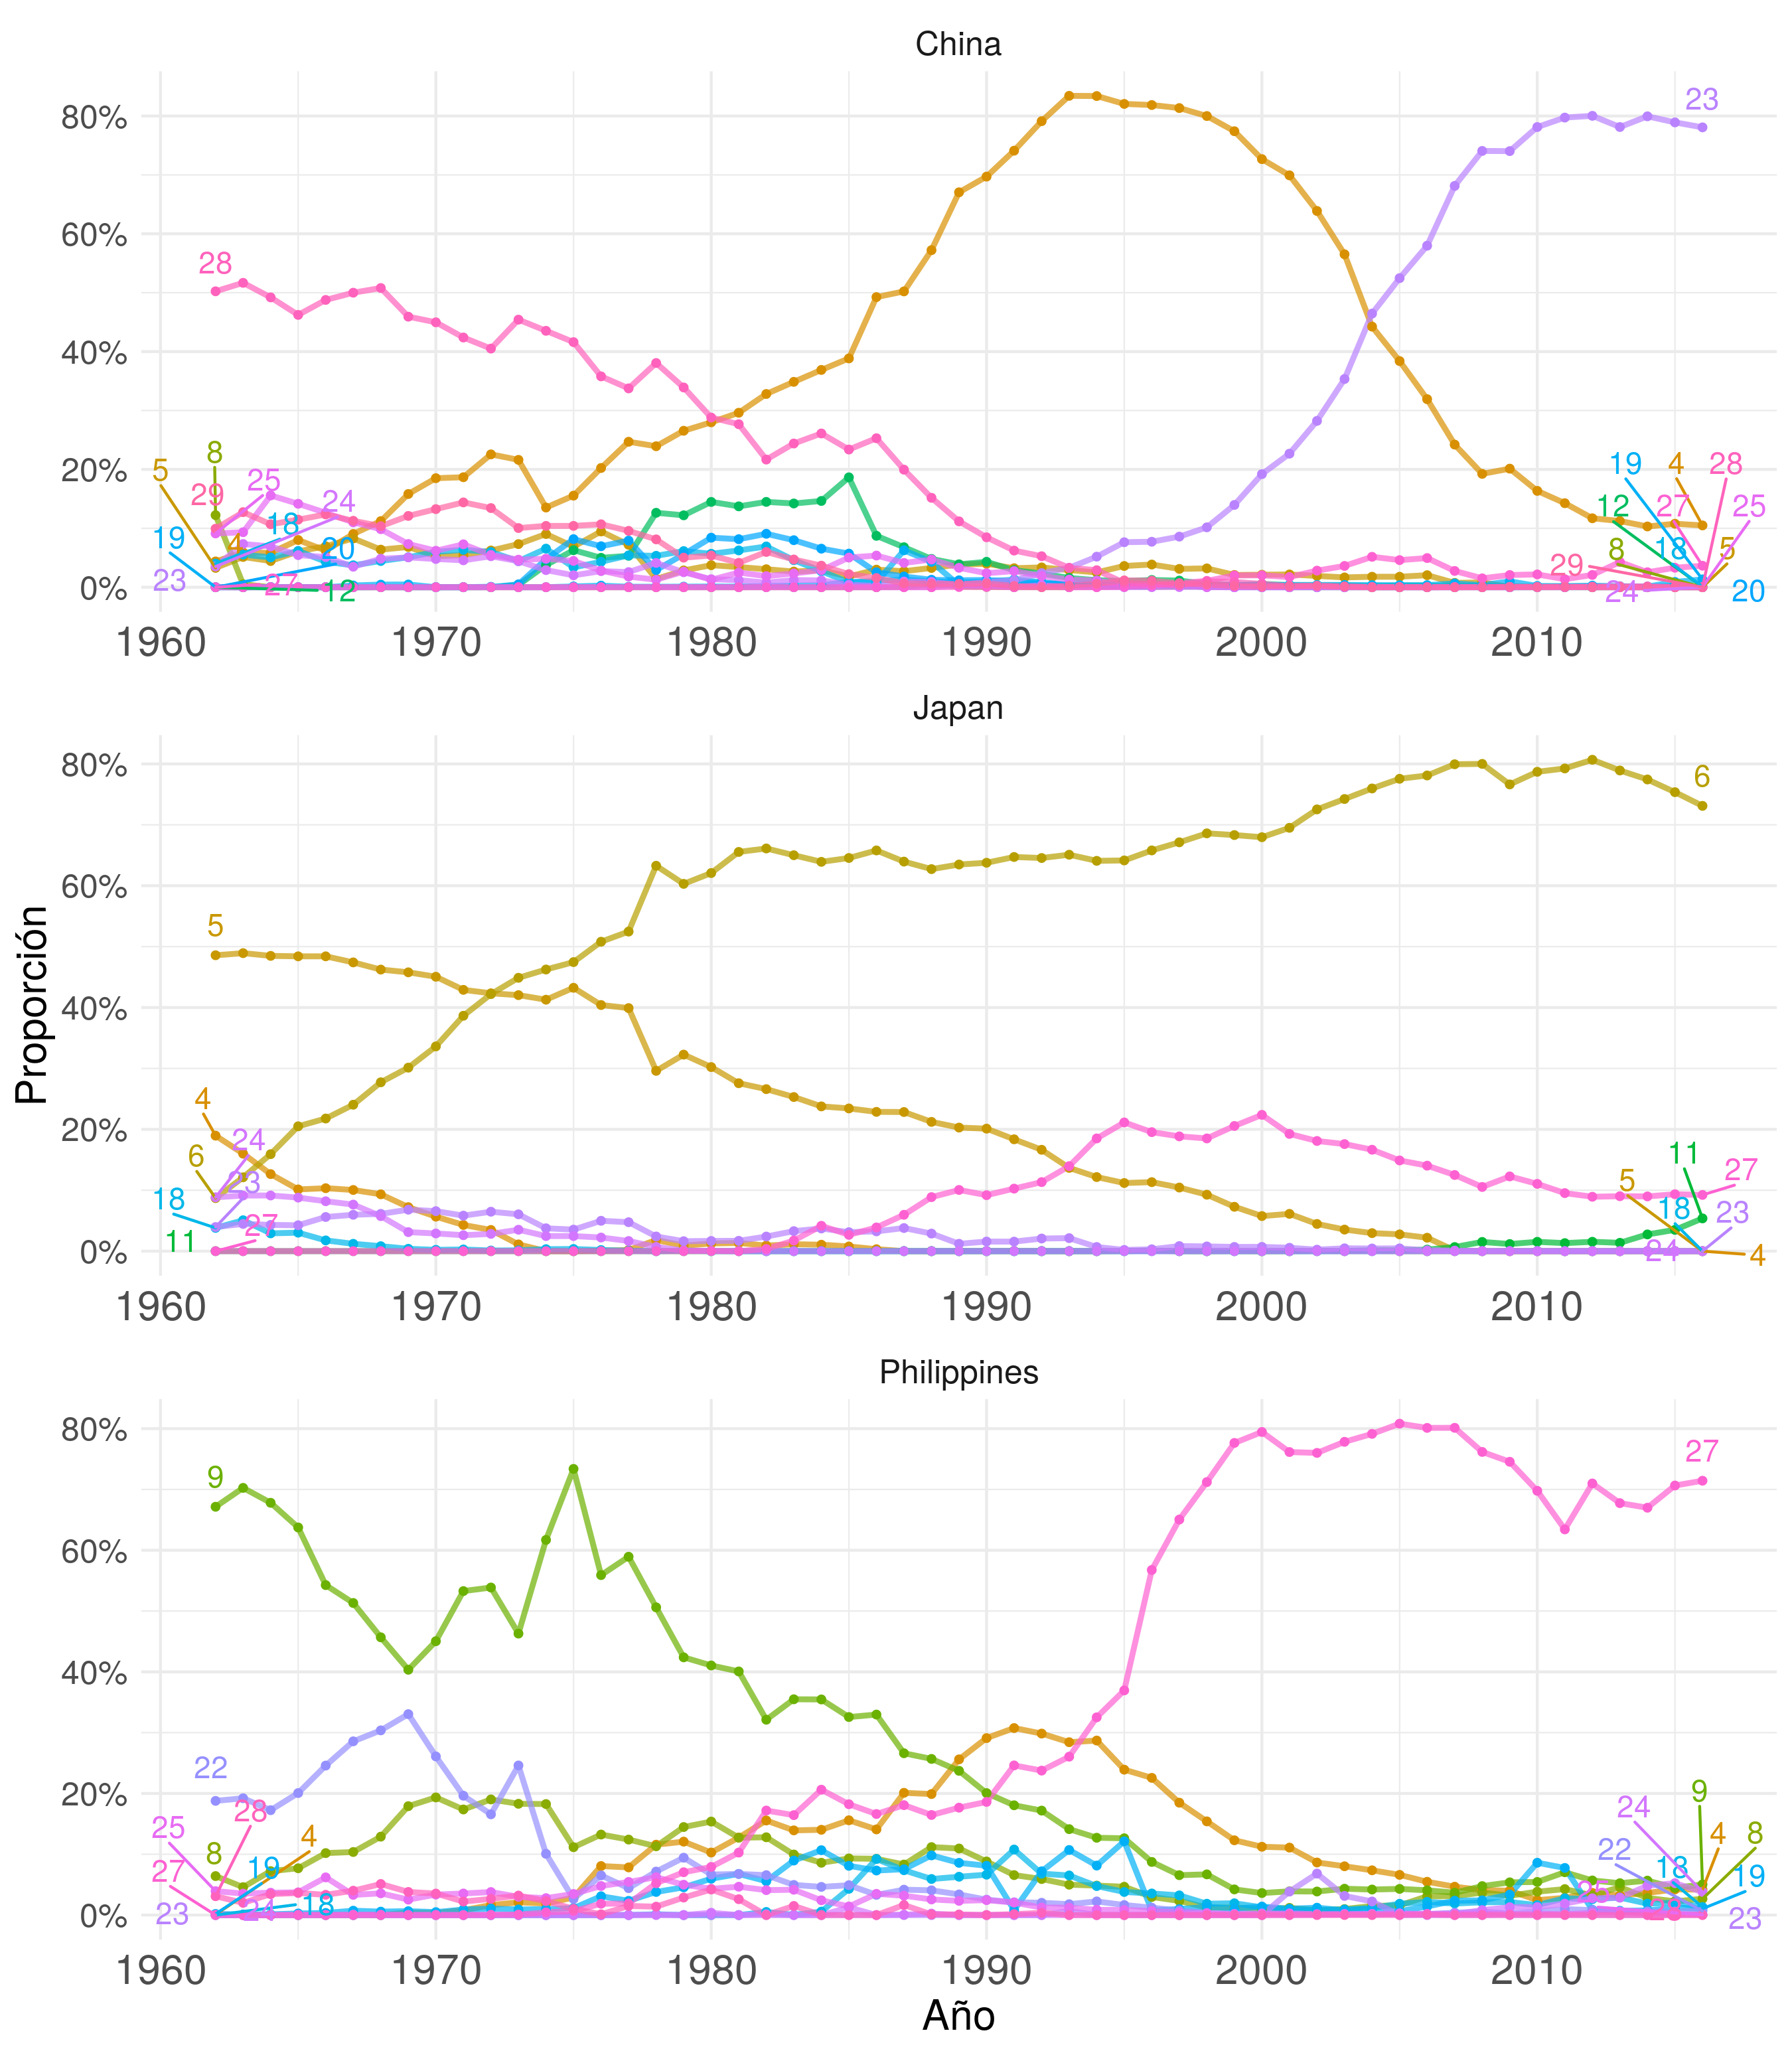
\includegraphics[width=\linewidth]{graficoLDA_k30_CHN_JPN_PHL}
\end{figure}

\column{.6\textwidth} % Left column and width

\begin{itemize}[label=\faRebel]
\item En \underline{China} se pueden observar \underline{tres etapas}: Hasta los 80' el componente 28 (\underline{Arroz, algodón, textiles}) era predominante. Entre 1980-2004 domina el componente 4 (textiles y juguetes), de \underline{industria de baja complejidad}. A partir de allí, el componente 23 (\underline{procesdaores, microcircuitos}, etc.). 
\item\underline{ Japón}, al igual que EUA, Francia y UK comienza la serie en el comp. 5, pero la caída en este caso es \underline{tendencial}, y se reemplaza por el 6 (vehículos, barcos, maquinarias y partes). 
\item En el caso de \underline{Filipinas}, hasta los 90' se especializa en productos \underline{agropecuarios} (Café, bananas, etc.) pasa brevemente por el componente 4, y rápidamente toma su lugar el 27(\underline{microcircuitos}).
\end{itemize}

\end{columns} 

En muchos países del sudeste asiático se ven, con matices, particularidades y distintas temporalidades, las tres etapas vistas en China y Filipinas. 

\end{frame}


\subsection{Grafo Bipartito}
\subsubsection{Metodología}

\begin{frame}
\centering
\Large Grafo Bipartito \\

\normalsize Metodología
\end{frame}

\begin{frame}


\begin{columns}[c] 

\column{.4\textwidth} % Right column and width
\centering
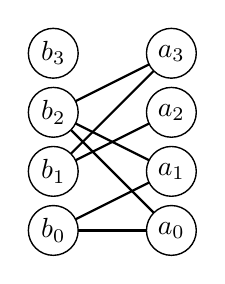
\begin{tikzpicture}[scale=0.75]

\begin{scope}[rotate=90]
\SetVertexMath
\grEmptyLadder[RA=1,RB=2]{4}   
\end{scope}
\Edges(b2,a0,b0,a1,b2,a3,b1,a2)
\end{tikzpicture} 

\column{.6\textwidth} % Left column and width
\small

\begin{itemize}[label=\faRebel]
\item Grafo bipartito entre países y productos
\item Se puede \underline{proyectar a un grafo de productos}, donde la relación de cercanía se define a partir de qué países los exportan
\item También se puede \underline{proyectar a un grafo de países}, donde la relación de cercanía surge por la similitud de sus canastas exportadoras.
\end{itemize}

\end{columns}

\end{frame}

\begin{frame}

\begin{columns}[c] 

\column{.4\textwidth} % Right column and width
$$
RCA(c,i)= \frac{\displaystyle \frac{x(c,i)}{\displaystyle \sum_{i}x(c,i)}}{\frac{\displaystyle\sum_{c}x(c,i)}{\displaystyle \sum_{c,i}x(c,i)}}
$$	
\column{.6\textwidth} % Left column and width

\small{
\begin{itemize}[label=\faRebel]
\item Para definir el punto de corte, se utilizó el concepto de \textit{Relative Comparative Advantages} basado en 	\cite{Hidalgo2009}.
\item Esto es, la proporción que representa un producto en la canasta exportadora de un país, respecto la proporción que representa en la canasta exportadora promedio mundial.
\end{itemize}
}
\end{columns}

\end{frame}


\begin{frame}

$$
\phi_{ij} = min (P(RCA_i>1/RCA_j>1),P(RCA_j>1/RCA_i>1)),
$$
\small

\begin{itemize}[label=\faRebel]
\item Para el\underline{ análisis de los productos}, nos basamos en el concepto de \textit{proximidad} de \cite{Hidalgo2009}.
\item $P(RCA_i/RCA_j)$ es la probabilidad condicional de exportar el producto $i$ dado que exporta el producto $j$.
\item $\Phi$ es por lo tanto una \underline{matriz de distancias} entre los productos. Esto resulta ideal para analizar los datos a través de la técnica de \underline{clustering} \textit{K-medioids} \citep{kaufman1987clustering}. El producto característico sirve para interpretar el cluster.
\end{itemize}

\end{frame}

\begin{frame}
Para el análisis del \underline{grafo proyectado de países}, se utilizo el \textit{clustering de Louvain} \citep{blondel2008fast} para detectar las comunidades de países que comparten una canasta exportadora similar.
\end{frame}

\subsubsection{Resultados}

\begin{frame}
\centering
\Large Grafo Bipartito \\

\normalsize Resultados
\end{frame}

\begin{frame}
\scriptsize 
\begin{figure}
\centering
\subfigure[Ordenado por nomenclador SITC]{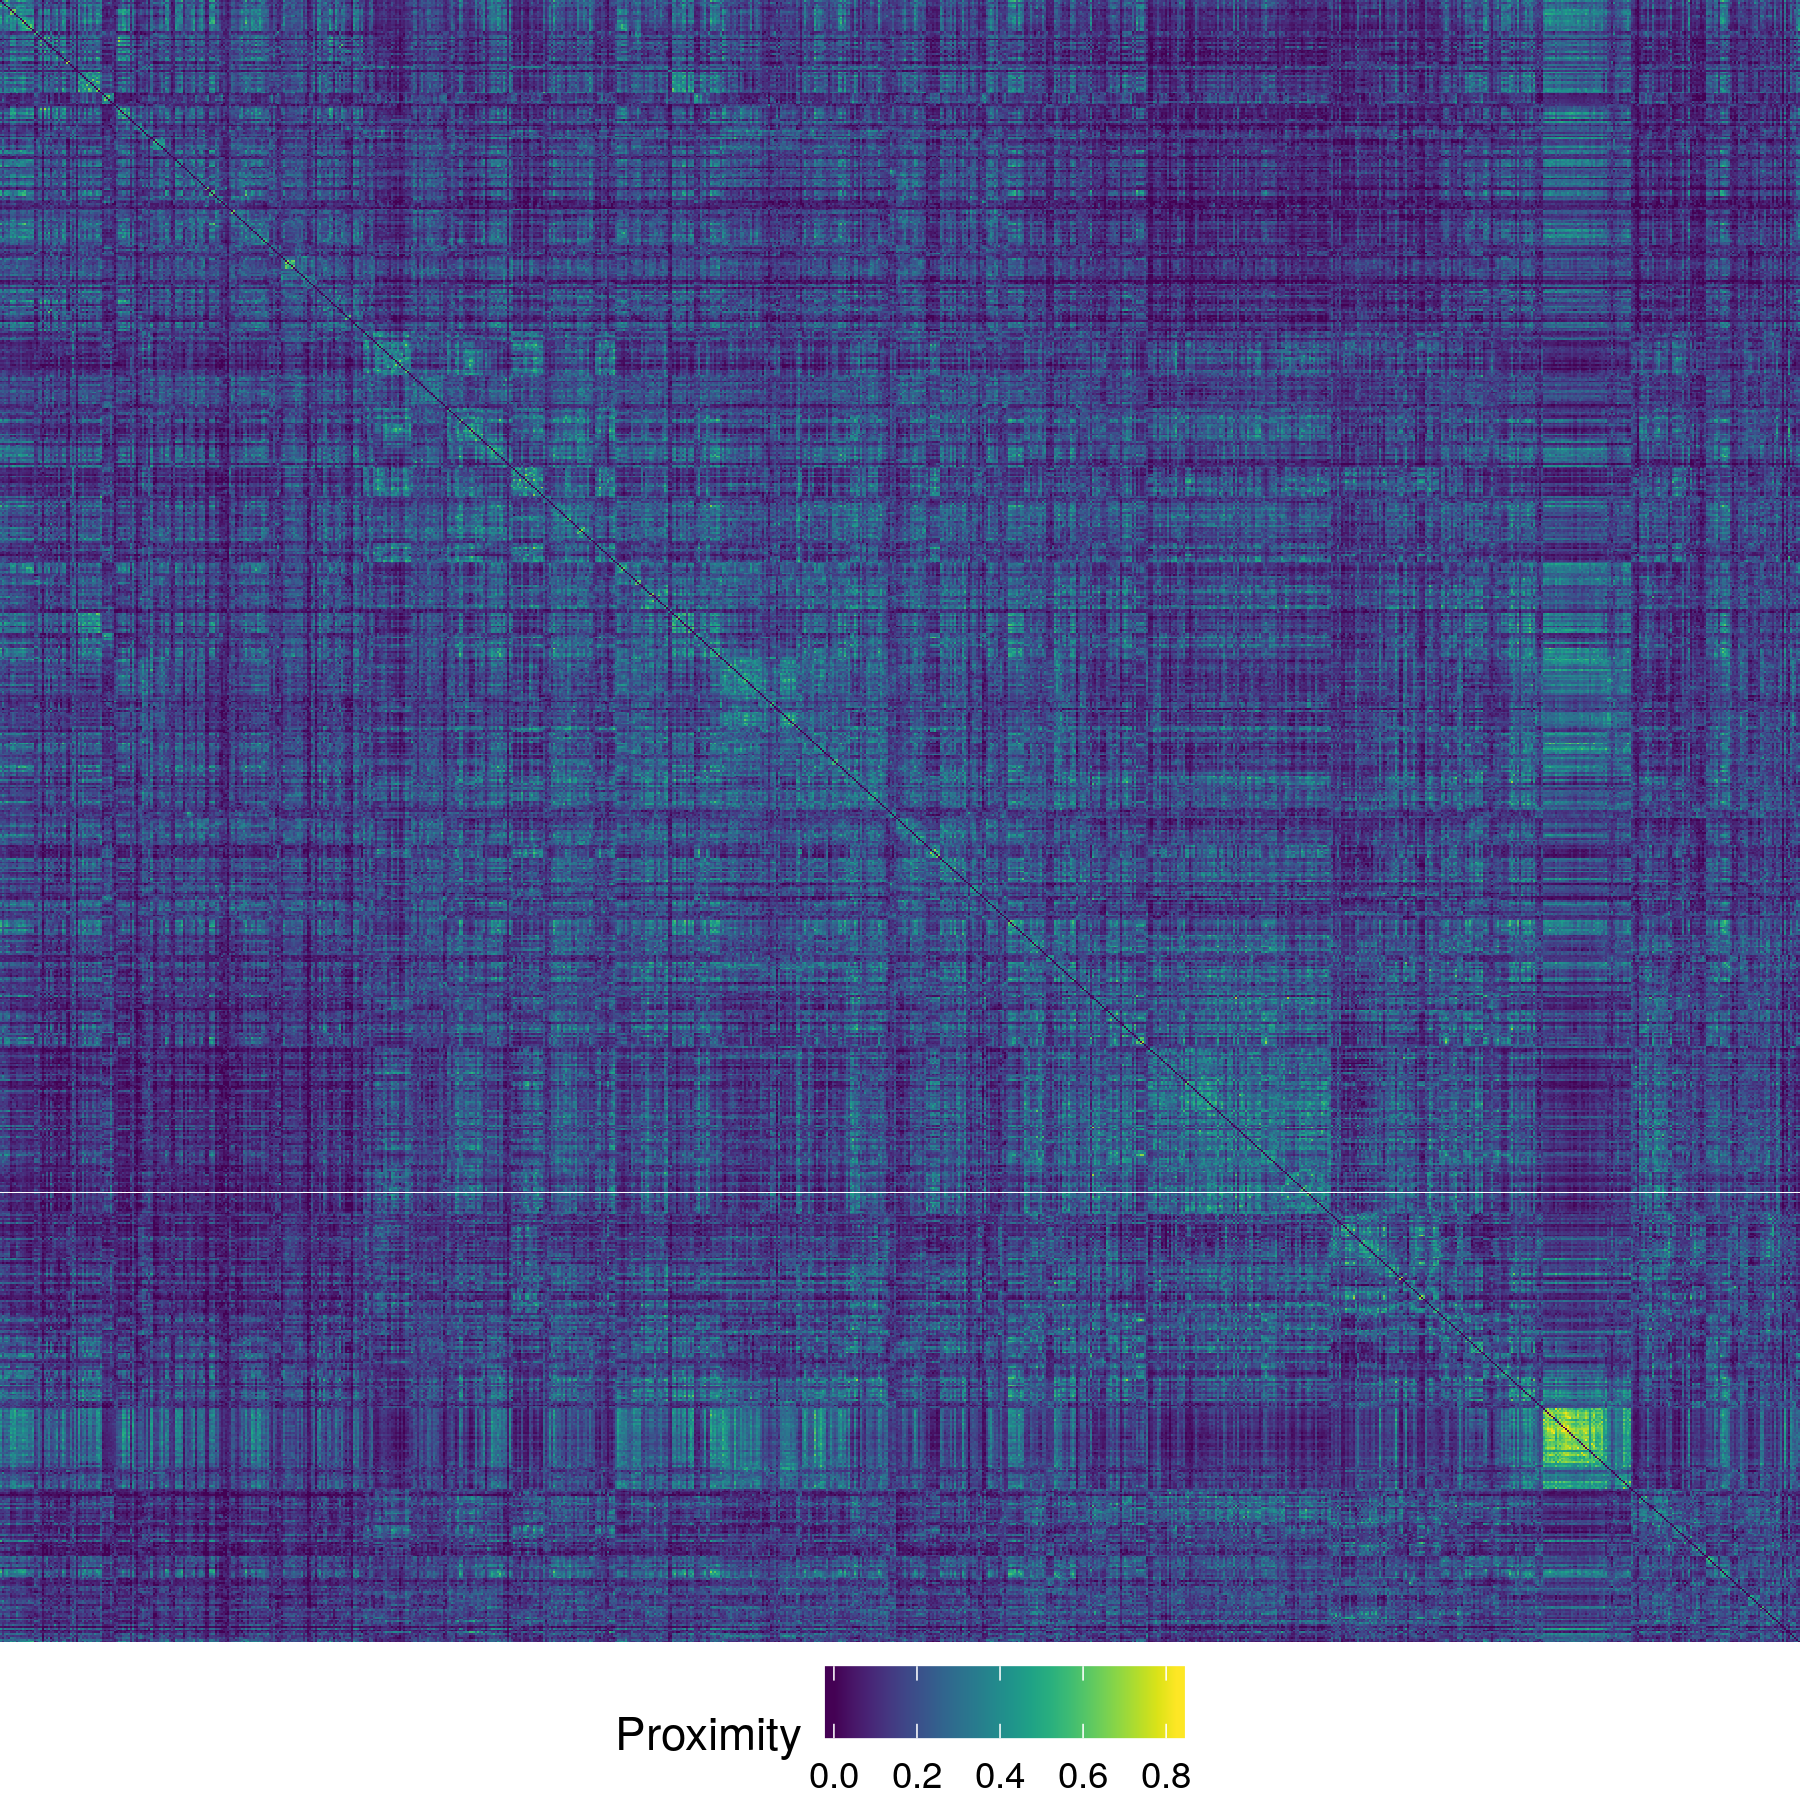
\includegraphics[width=.45\linewidth]{Graficos/heatmap_prox_sitcOrd}}
\subfigure[Ordenado por clustering]{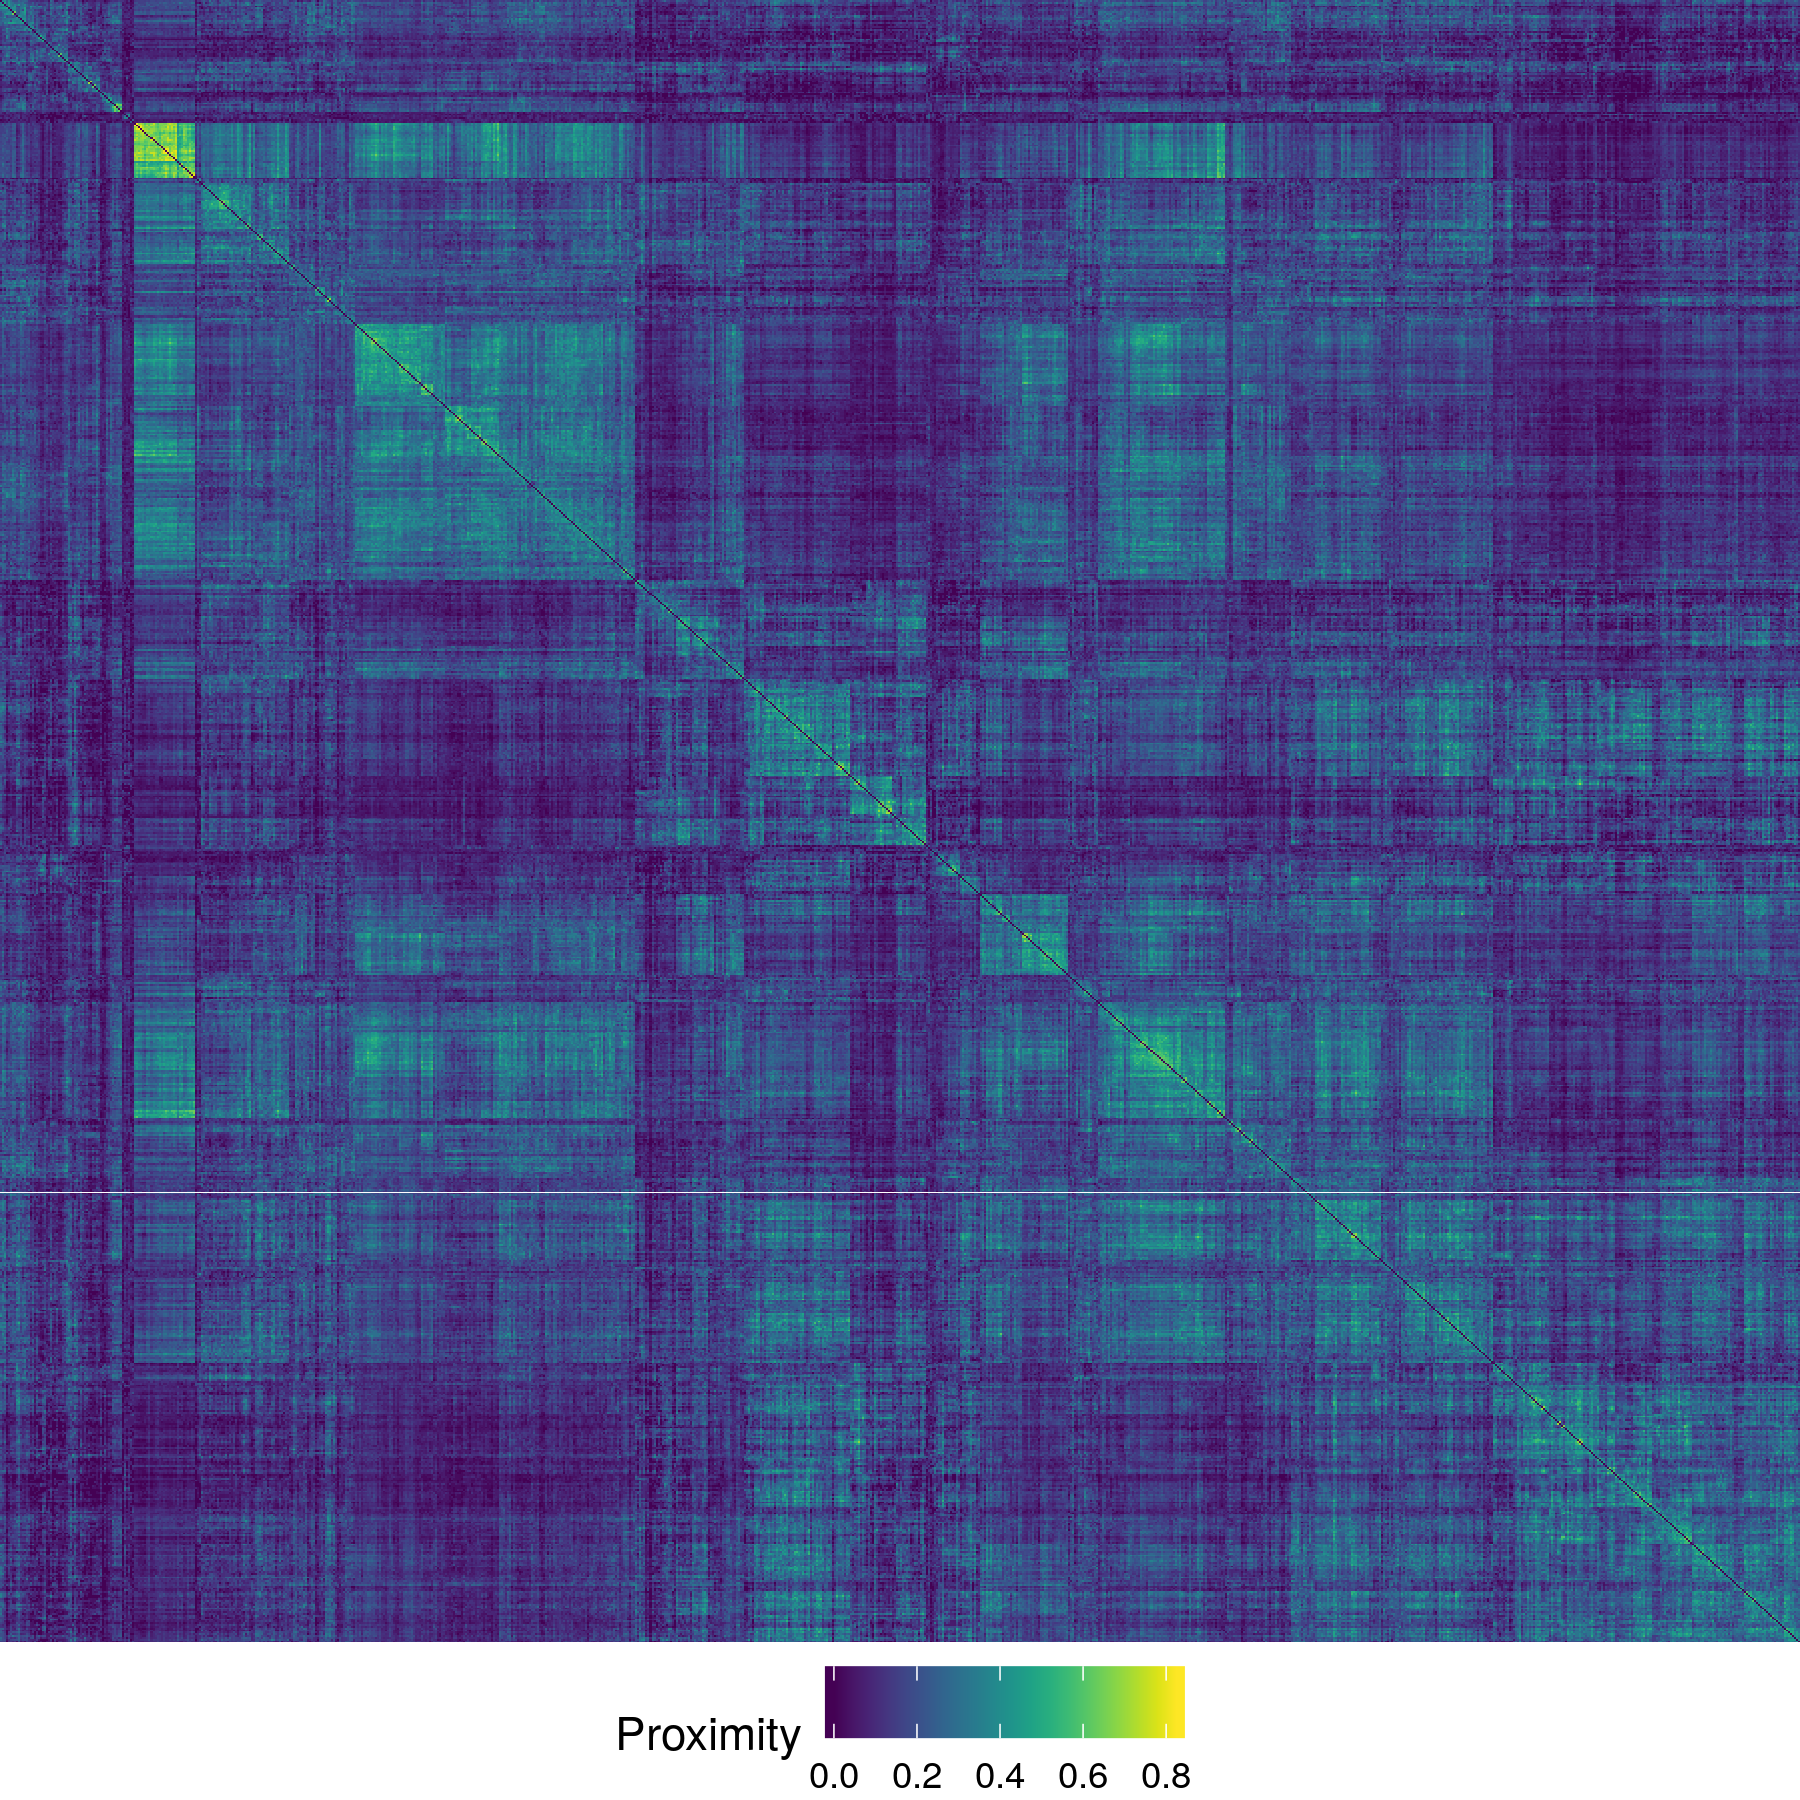
\includegraphics[width=.45\linewidth]{Graficos/heatmap_prox_ClustOrd}}
\caption{Heatmap proximidad}
\end{figure}

\end{frame}

\begin{frame}
\small{Componente gigante. Grafo de proximidad y clustering por K-medioides. Exportaciones. Promedio 1996-2017. 10 medioides}
\begin{columns}[c] 

\column{.5\textwidth} % Right column and width

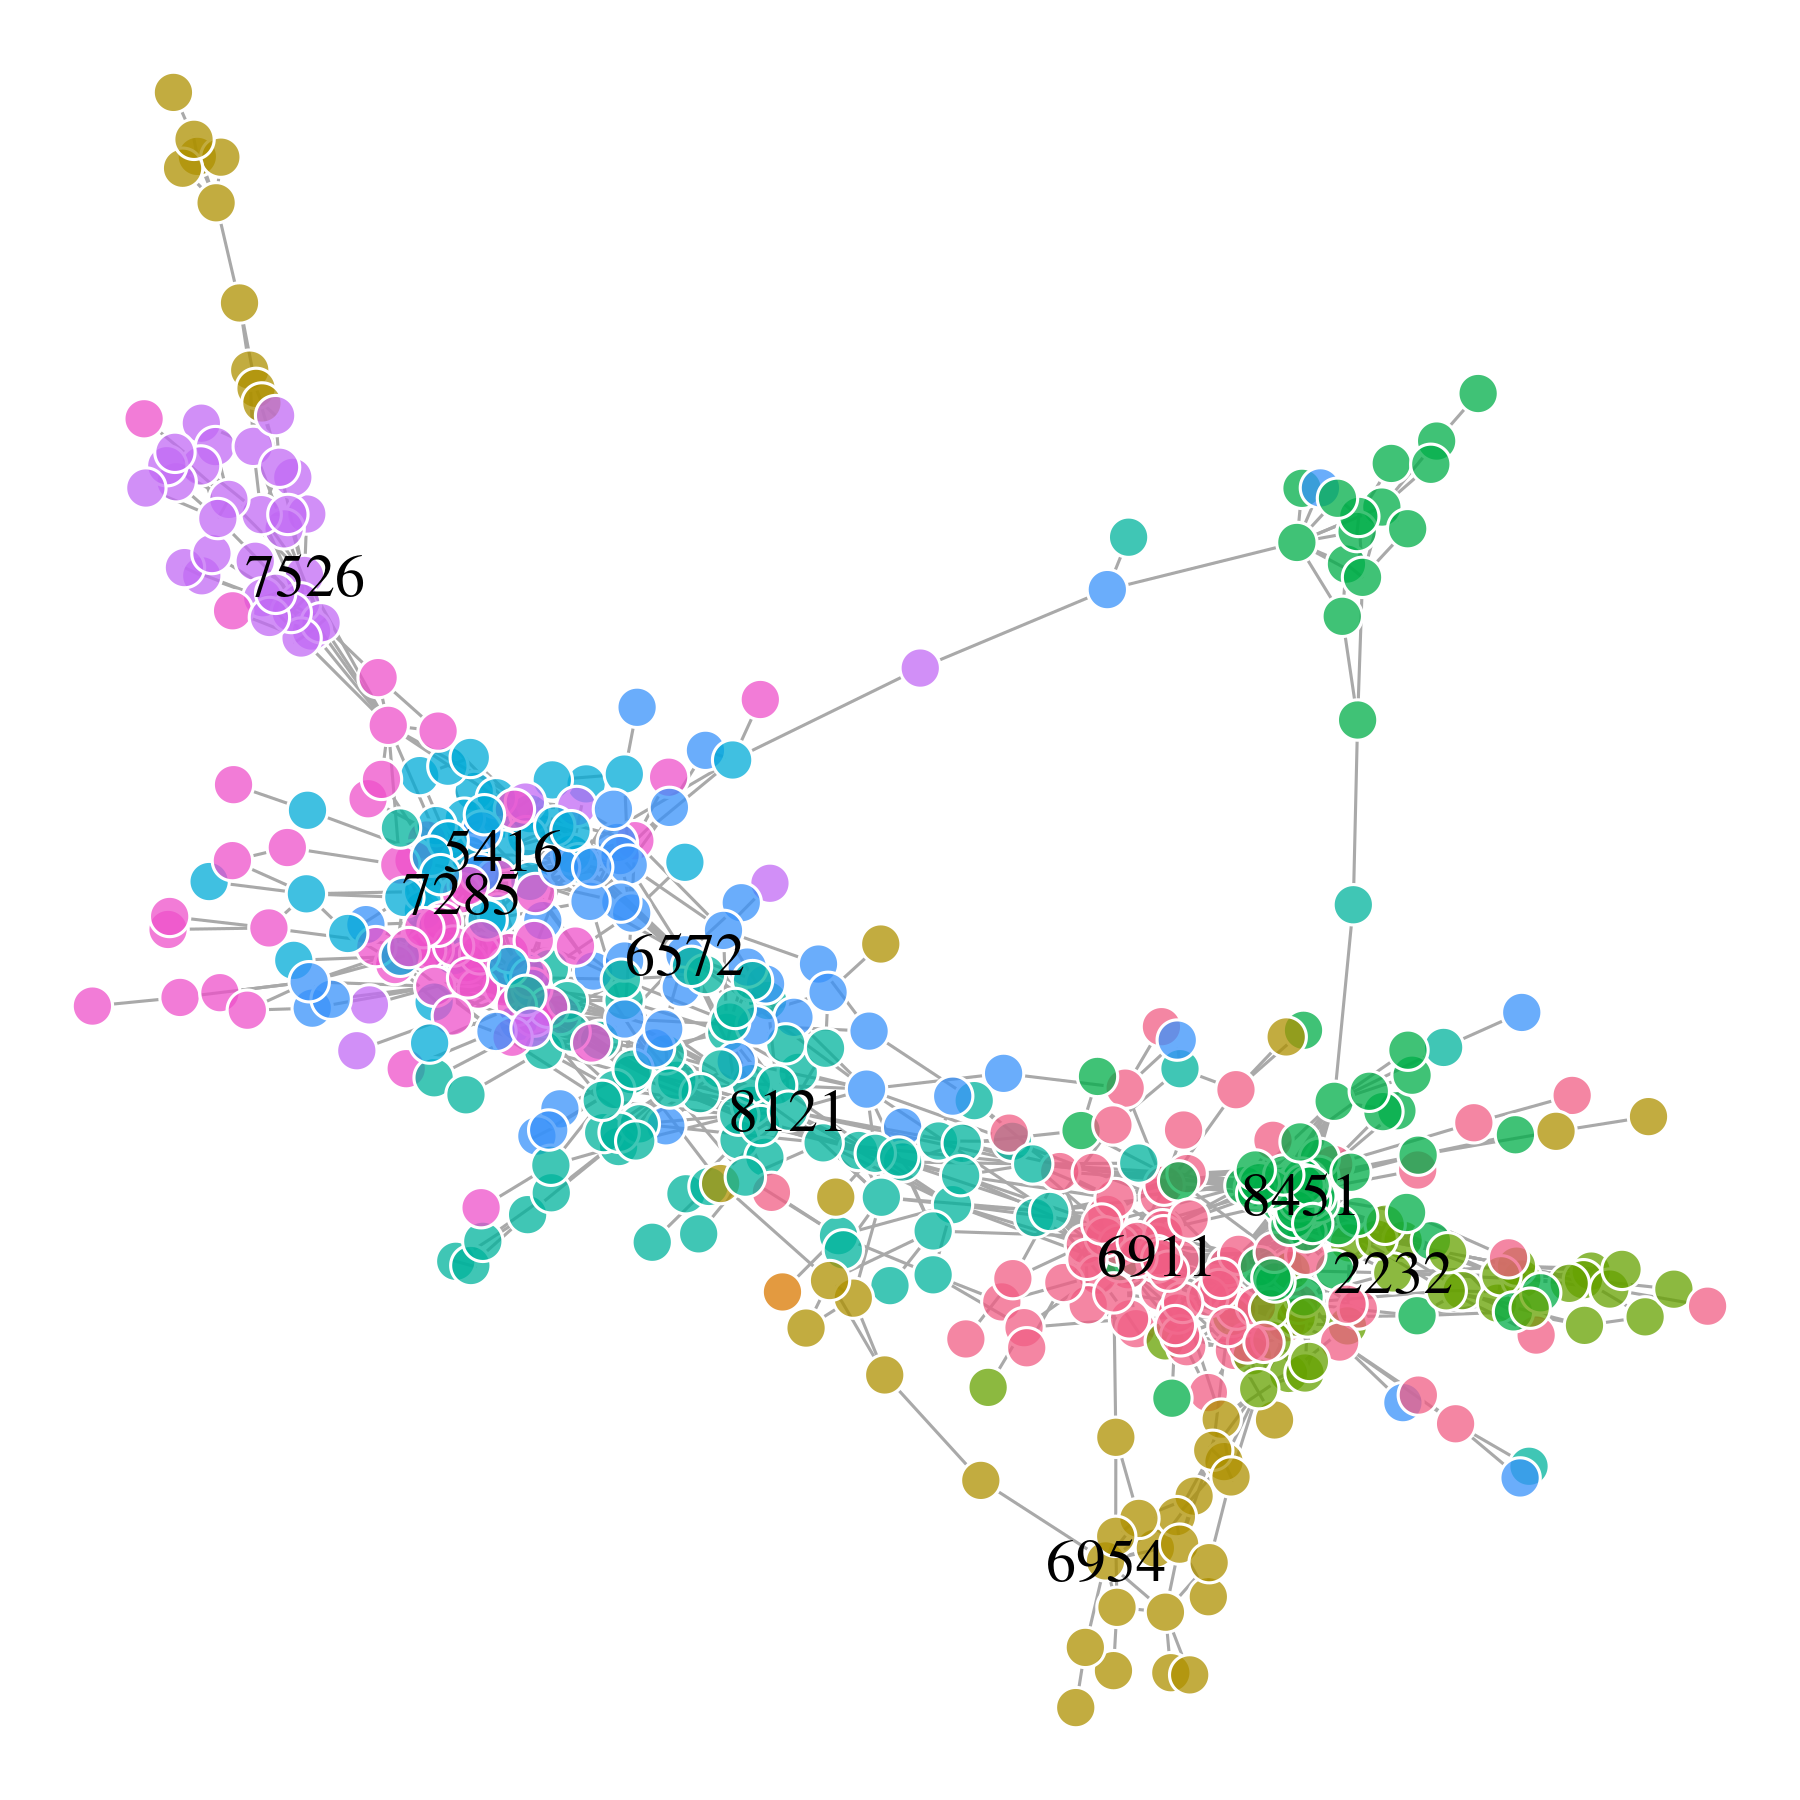
\includegraphics[width=\linewidth]{pam10_gigant}

\column{.5\textwidth} % Left column and width

\tiny
\begin{table}
\centering
\begin{tabular}{ll}
\hline
medioide & Description \\ 
\hline
6911 & Metal structures,parts \\ 
2831 & Copper ores and concentrates \\ 
6954 & Hand tools,etc. nes \\ 
2232 & Palm nuts and kernels \\ 
8451 & Babies'garmnts,clths acc \\ 
8121 & Boilrs.radiatrs,etc.n.el \\ 
5416 & Glycosides; glands etc. \\ 
6572 & Non-wovens, whether or not impregnated \\ 
7526 & ... units for automatic data processing \\ 
7285 & Parts publc wrk mach etc \\ 
\hline
\end{tabular}
\end{table}

\end{columns}

\end{frame}


\begin{frame}

\begin{itemize}[label=\faRebel]
\item El ordenamiento por proximidad permite una \underline{mejor organización} que por el nomenclador tradicional (SITC\citep{WTO2017})
\item En la proyección del espacio de productos se observan \underline{algunos clusters bien diferenciados}, como el de microcircuitos(7526) y el de herramientas(6954). Sin embargo, los demás no son claramente separables, y su interpretación, al estar atada a un solo producto, es más compleja.

\end{itemize}
\end{frame}


\begin{frame}
\begin{figure}
\centering
\subfigure[1966]{\label{fig:mapas_proyeccion_1}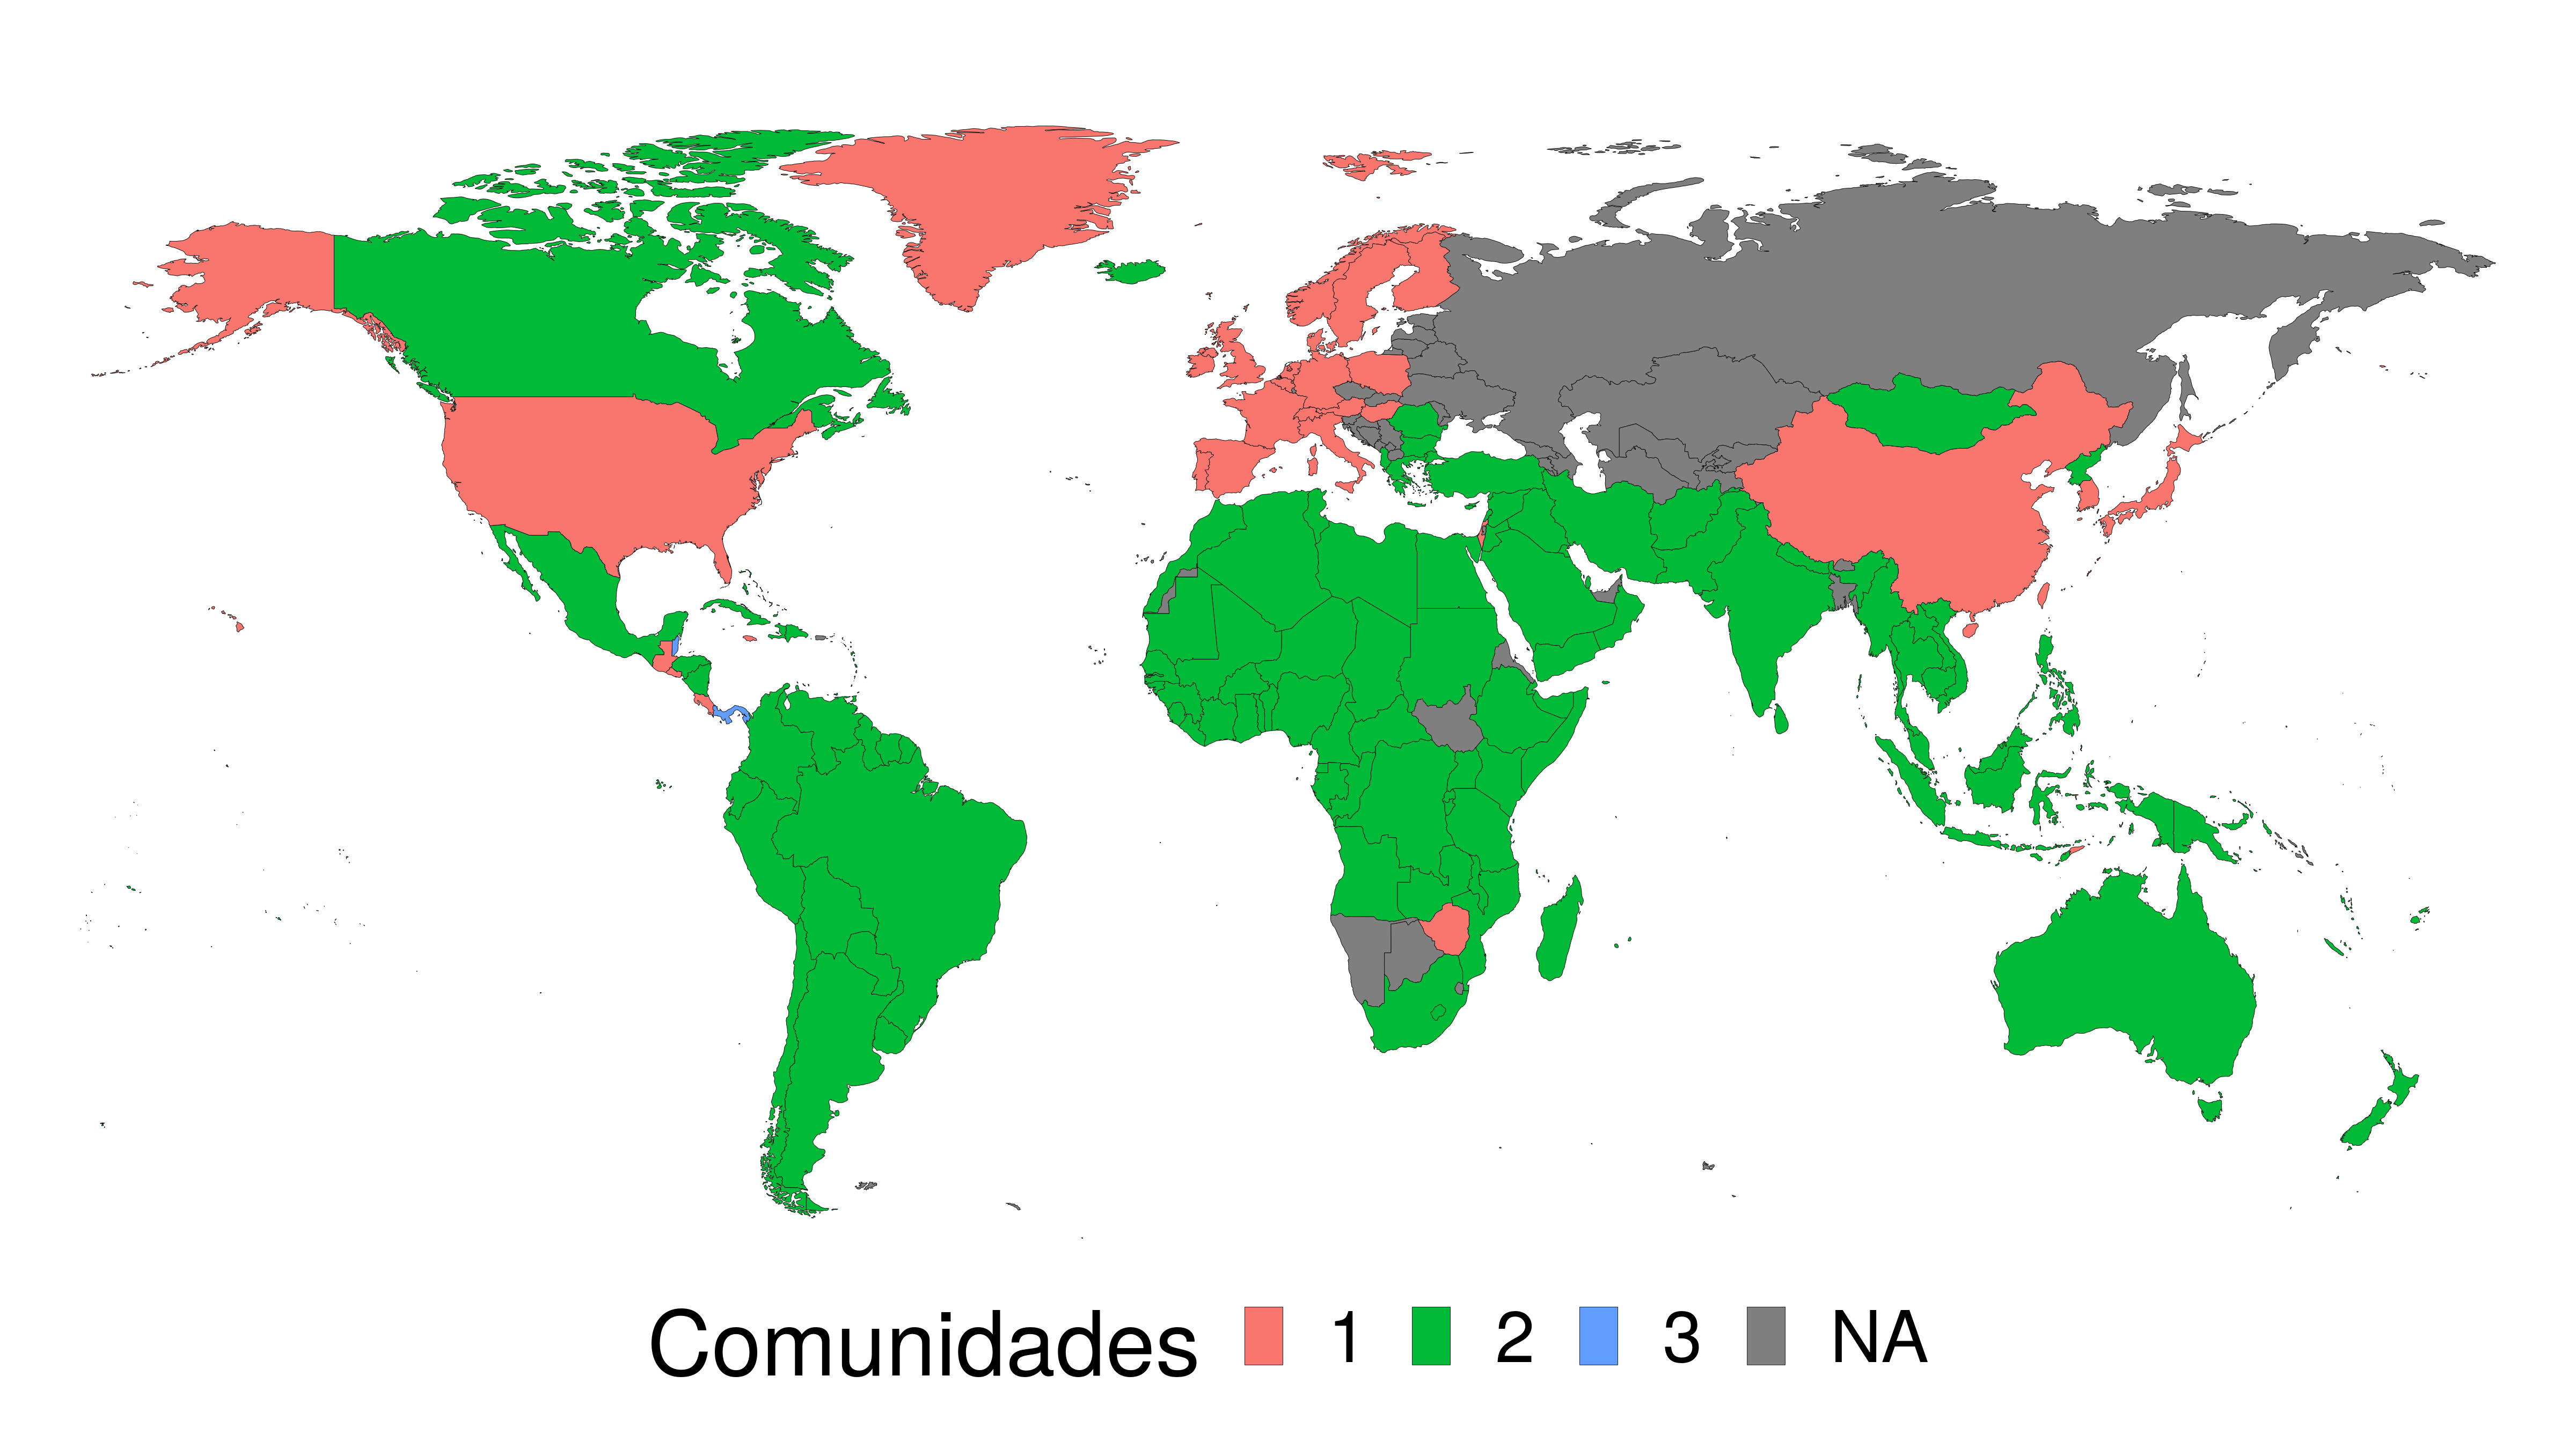
\includegraphics[width=0.45\linewidth]{mapa_projection_louvain_lp_1966}}
\subfigure[1986]{\label{fig:mapas_proyeccion_3}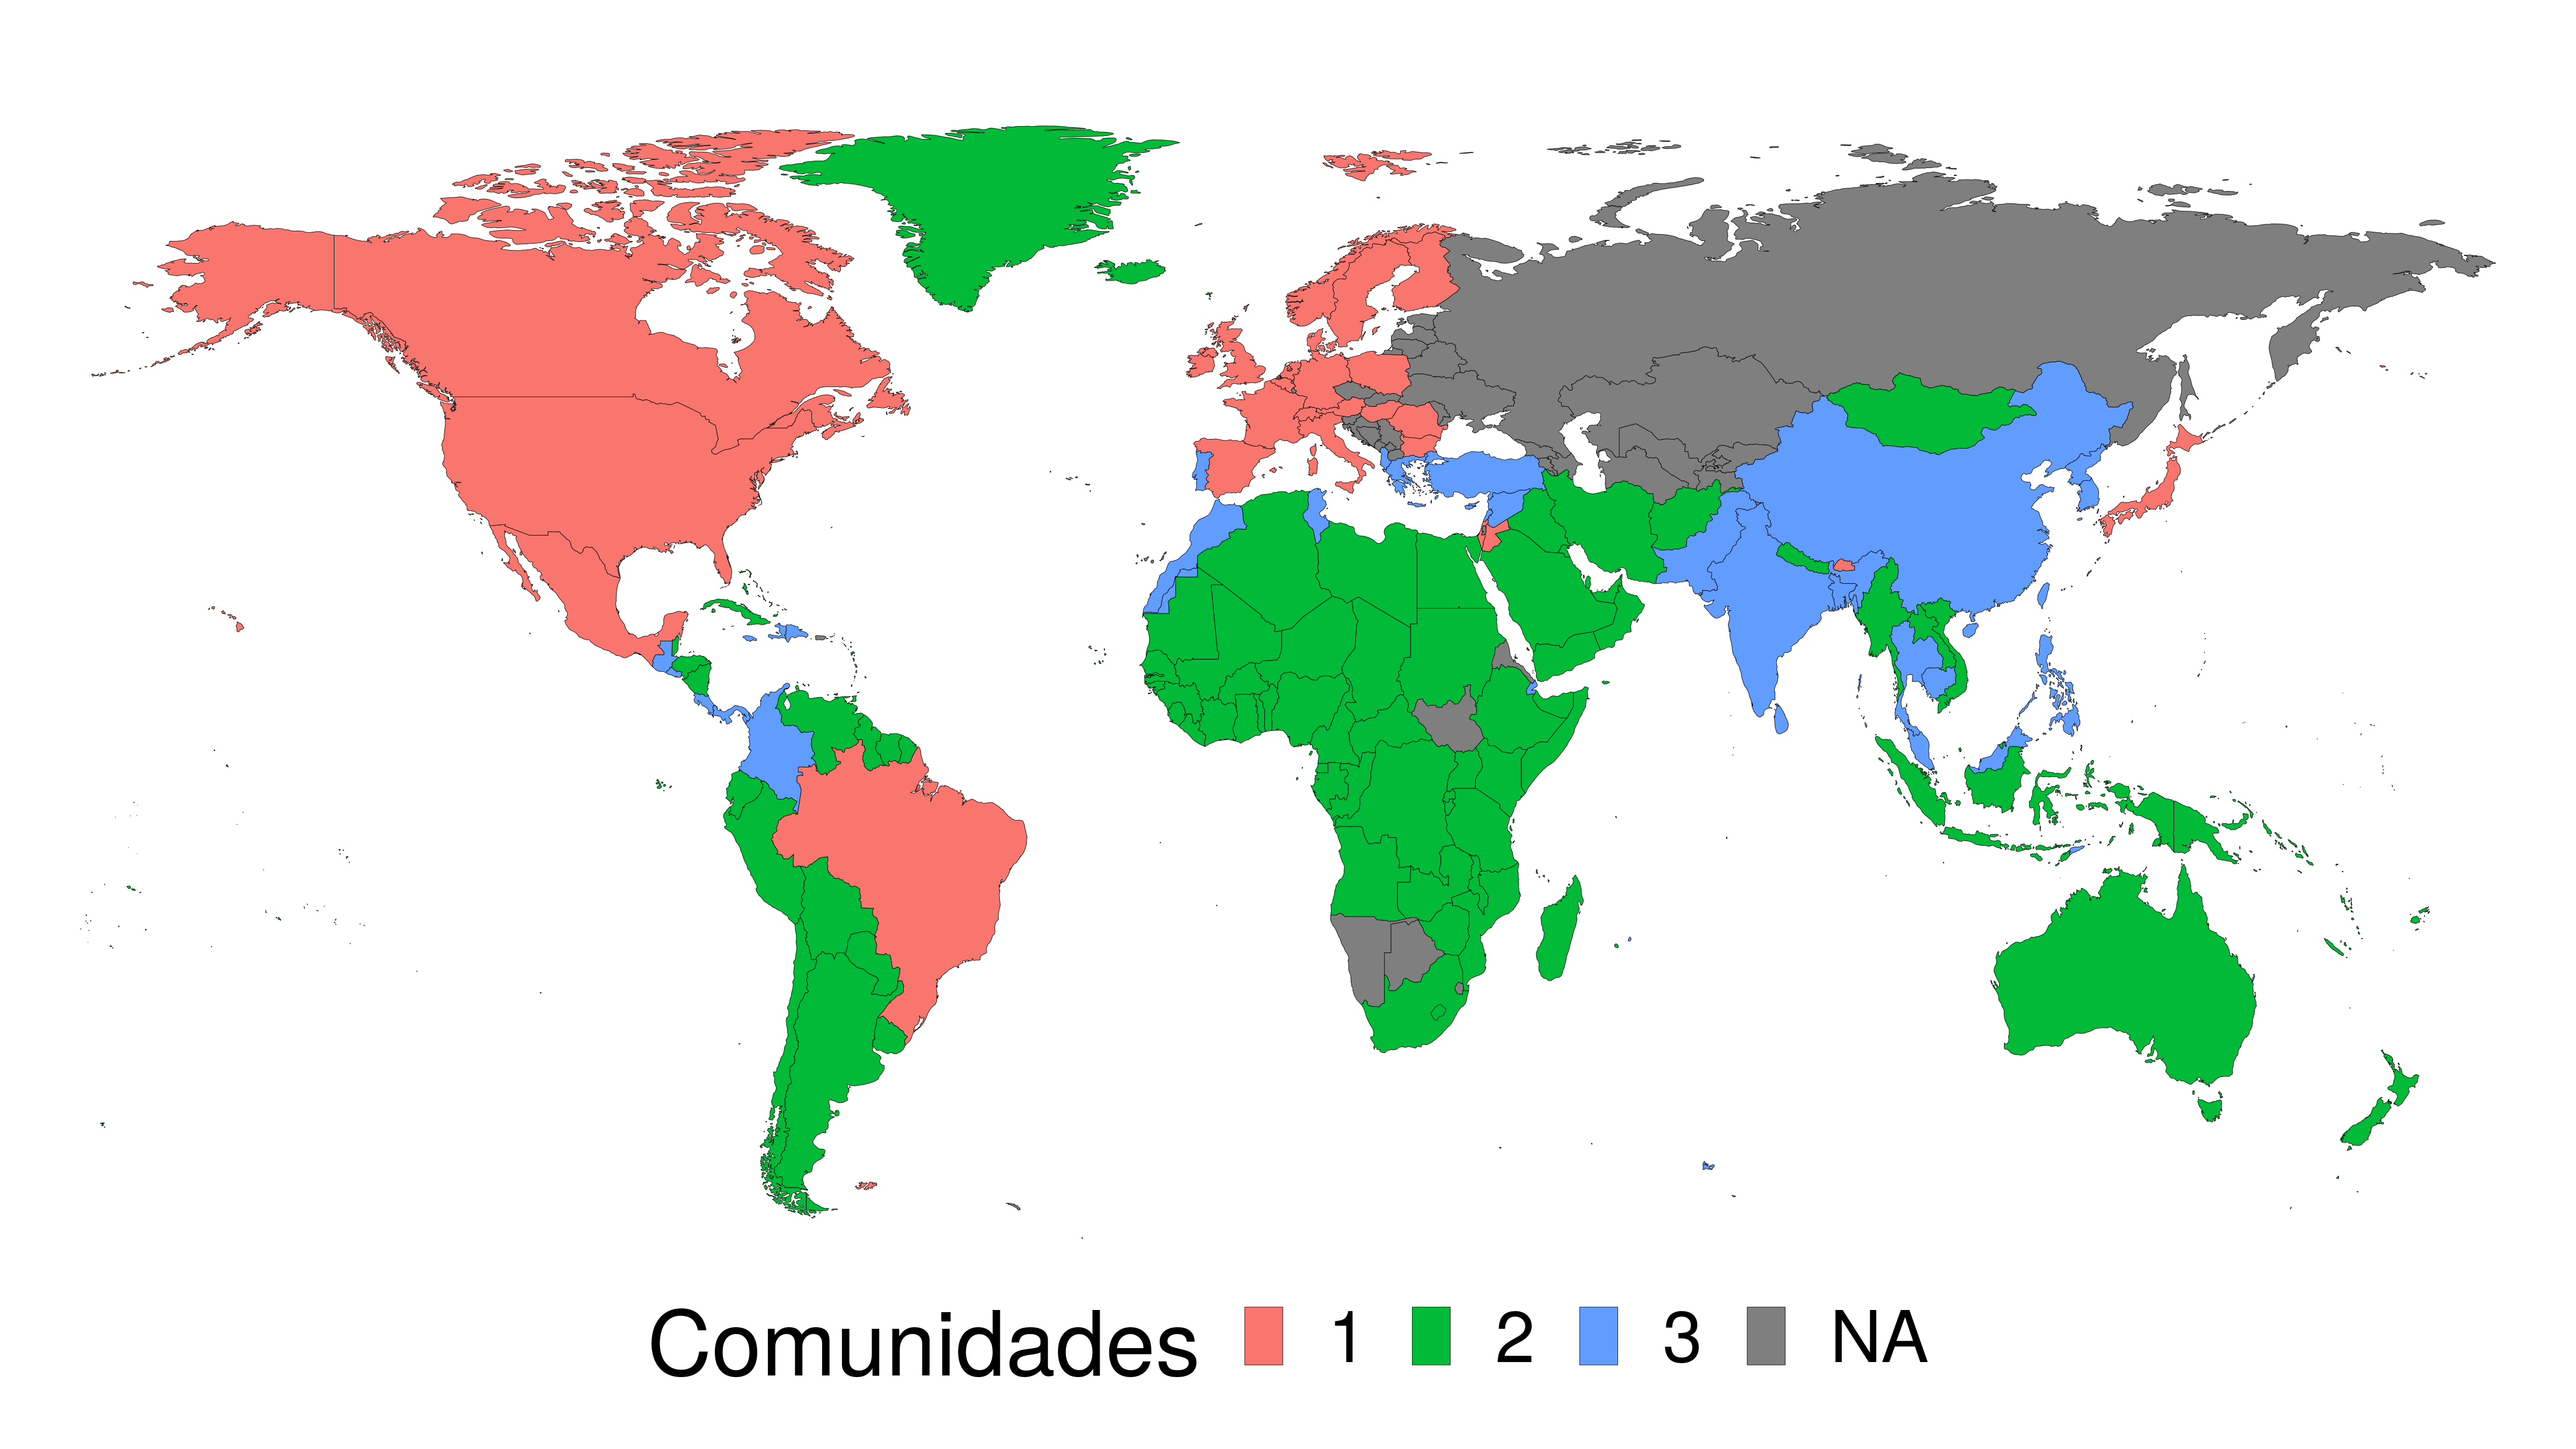
\includegraphics[width=0.45\linewidth]{mapa_projection_louvain_lp_1986}}
\subfigure[2016]{\label{fig:mapas_proyeccion_5}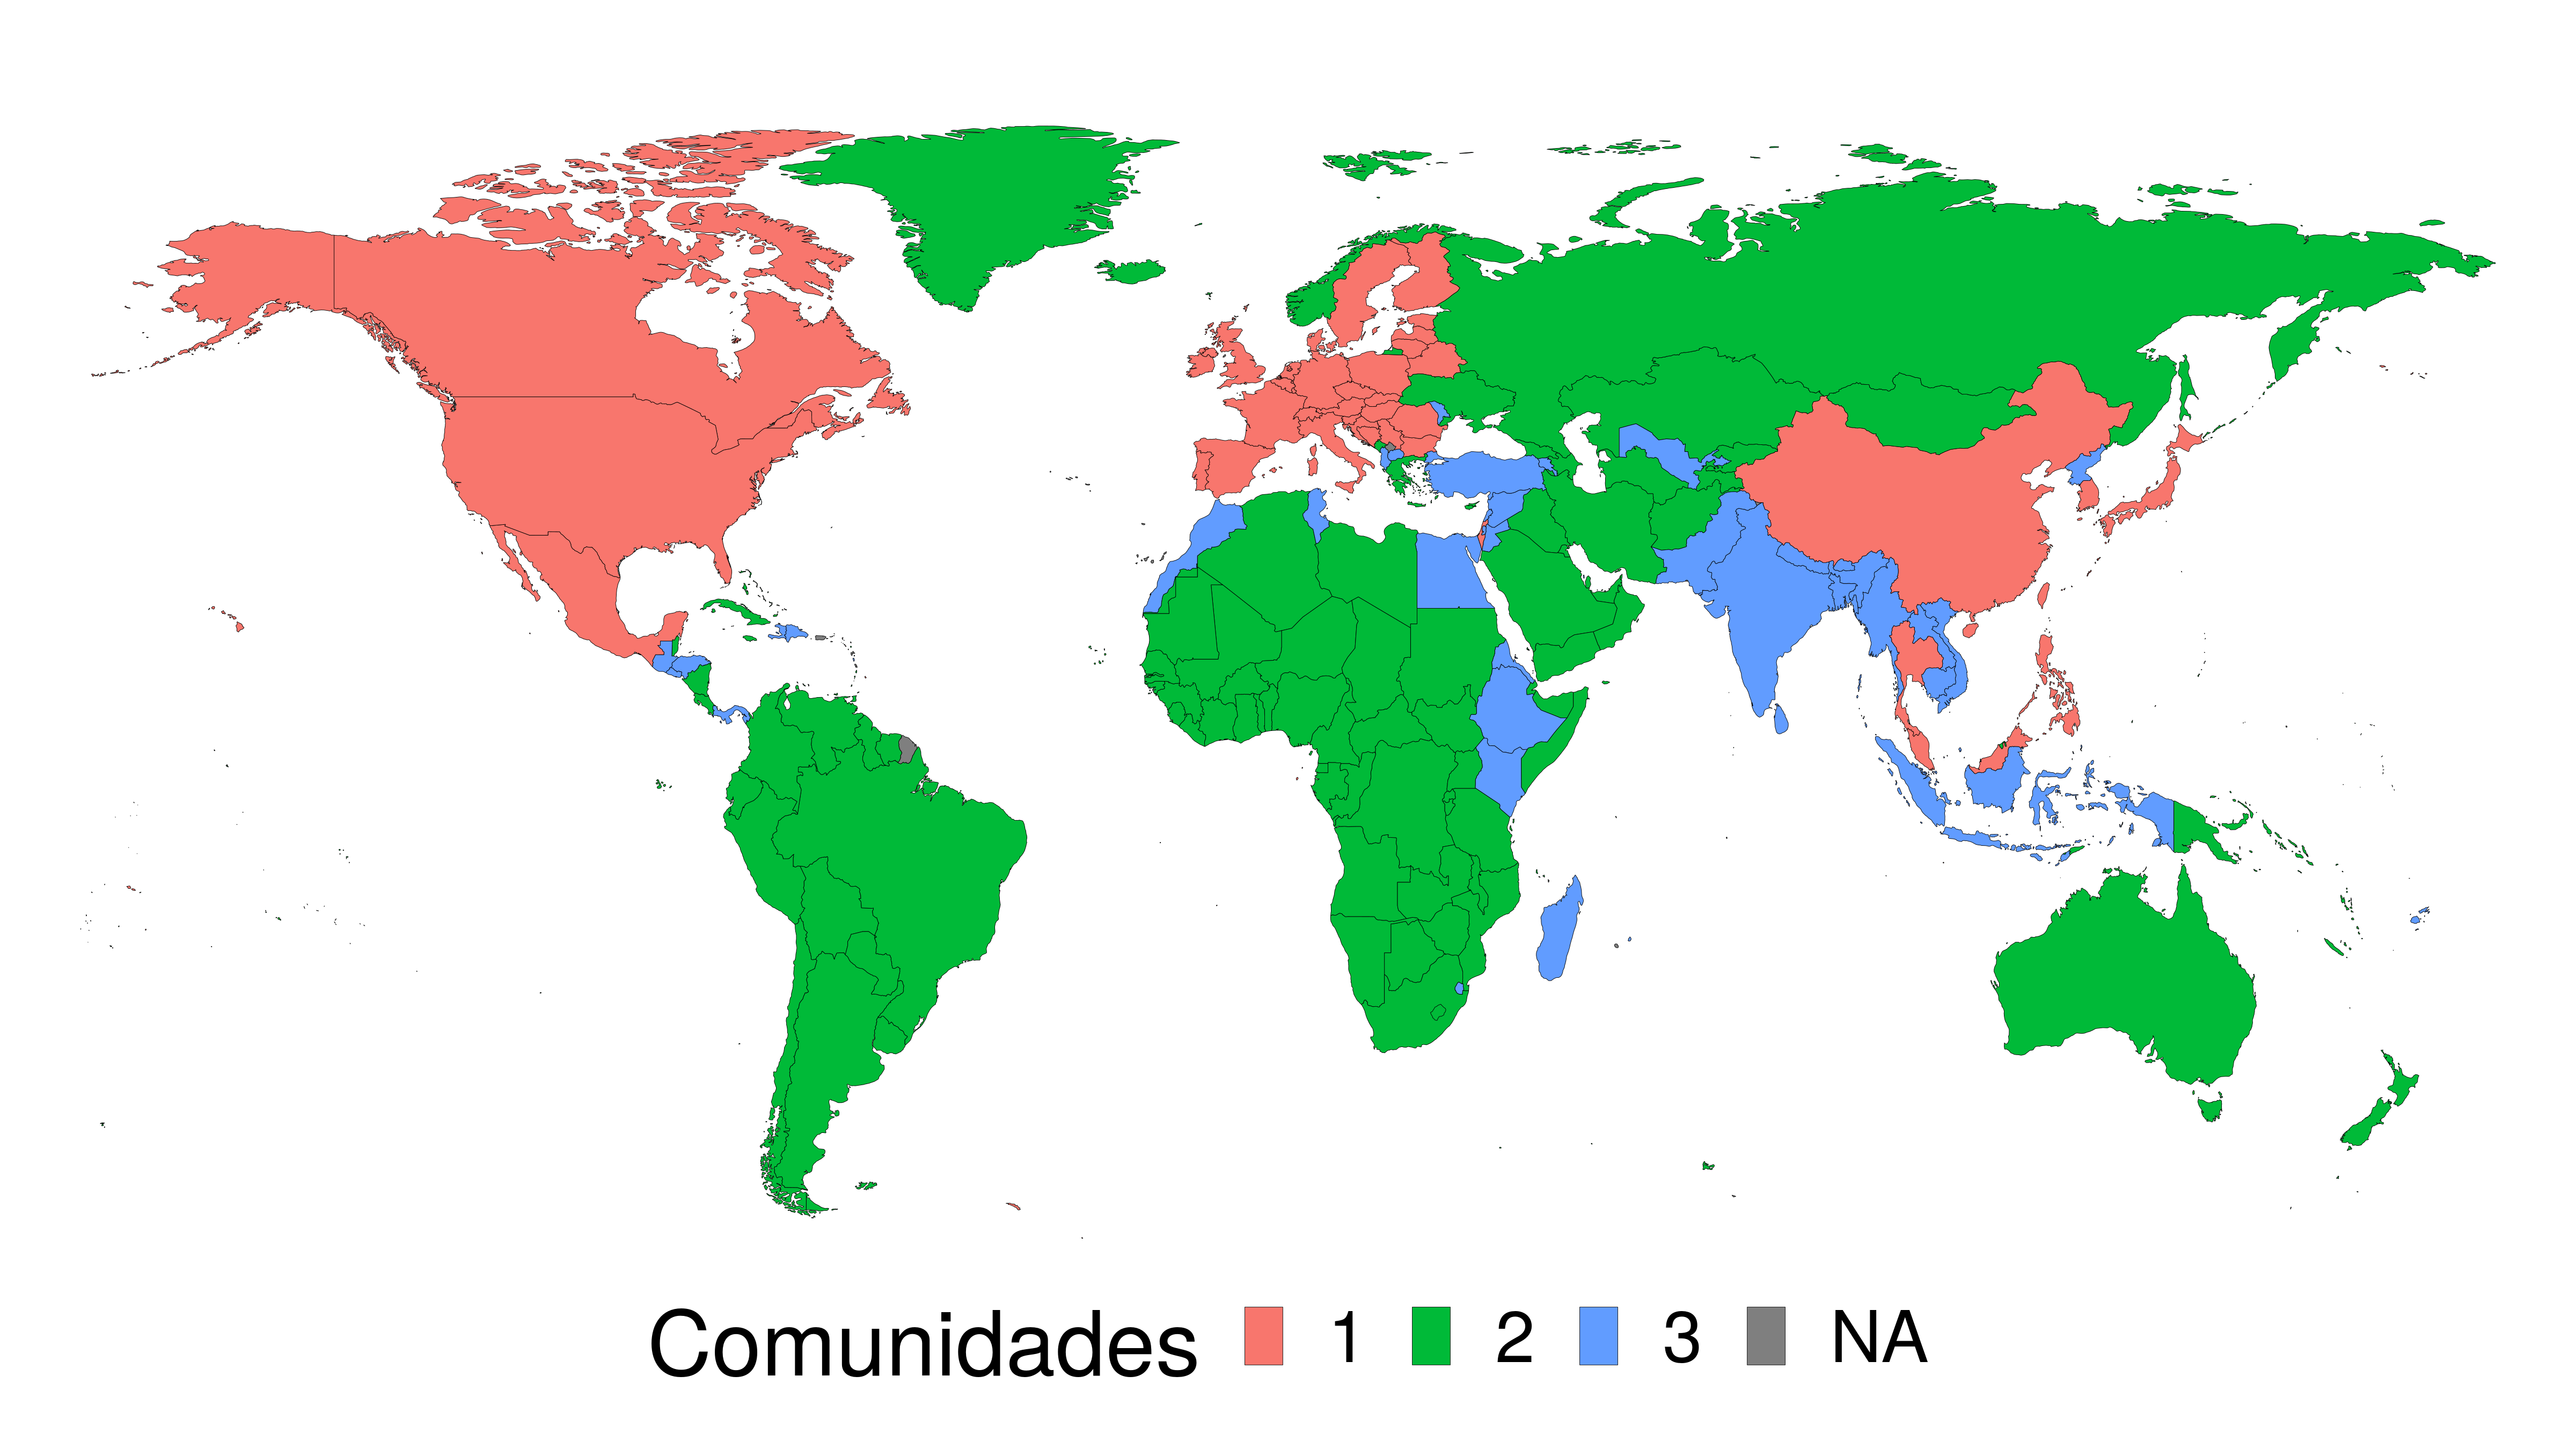
\includegraphics[width=0.5\linewidth]{mapa_projection_louvain_lp_2016}}
\caption{Proyección a países del grafo bipartito. Clustering Louvain. Exportaciones}
\label{fig:mapas_proyeccion_louvain}
\end{figure}
\end{frame}



\begin{frame}
\begin{itemize}[label=\faRebel]
\item En la proyección al grafo de países se pueden ver, a grandes rasgos, los cambios en la división internacional del trabajo: 
\begin{itemize}
\item En \underline{1966} el mundo tiene \underline{dos grandes grupos}: industriales y agropecuarios
\item En \underline{1986} se constituye un tercer cluster de países del \underline{Sudeste Asiático} (China, Pakistán, India, Filipinas, Thailandia, Malasia, etc.)
\item en \underline{2016}, en el Sudeste Asiático se suman países al tercer cluster, mientras que otros (China, Tailandia, Malasia, Filipinas) pasan al cluster de Europa, EEUU y Japón.
\end{itemize}

\end{itemize}
\end{frame}

\section{Conclusiones}

\small

\begin{frame}
\frametitle{Comercio Agregado}
\begin{itemize}[label=\faRebel]
\item El grafo simple de comercio agregado entre países nos permite caracterizar las \underline{relaciones asimétricas} en el comercio internacional
\item Según el punto de vista de exportaciones e importaciones, se puede ver el rol de los países en tanto \underline{\textit{productores} y \textit{consumidores}} de mercancías en el mercado mundial. 
\end{itemize}
\end{frame}

\begin{frame}
\frametitle{Comercio Agregado}
\begin{itemize}[label=\faRebel]

\item Por el método de construcción, al integrar el punto de corte como variable, podemos observar \underline{relaciones de dependencia} entre países.
\item Las medidas de \underline{clustering} y \underline{correlación} del grafo nos permiten caracterizar la \underline{evolución} de las formas generales del comercio mundial.
\item La evolución en el tiempo de las medidas de \underline{centralidad} nos permite observar los \underline{cambios en los \textit{grandes jugadores}} del comercio internacional.

\end{itemize}
\end{frame}


\begin{frame}
\frametitle{LDA}
\begin{itemize}[label=\faRebel]
\item Al utilizar la información \underline{desagregada a nivel producto} encontramos que el análisis se enriquece, pero también que la multiplicidad de dimensiones de estudio complejizan la lectura de la información. 
\item La metodología propuesta de \underline{\textit{Topic Modeling}} implica la construcción de un nomenclador \textit{agnóstico}, exclusivamente basado en los datos.
\end{itemize}
\end{frame}

\begin{frame}
\frametitle{LDA}
\begin{itemize}[label=\faRebel]

\item LDA Logra dar cuenta de la \underline{especificidad} \underline{de la canasta exportadora} de los países, y su evolución, con un grado de detalle que permite corroborar una multiplicidad de fenómenos reconocidos en la literatura
\item Lograr resumir en un único sistema de indicadores una caracterización del comercio mundial con cierto nivel de detalle permite \underline{evitar sesgos de selección de indicadores}.
\end{itemize}
\end{frame}

\begin{frame}
\frametitle{Grafo bipartito}
\begin{itemize}[label=\faRebel]
\item Como contraste a LDA, se elaboró una variación de la línea de trabajo de \cite{Hidalgo2007} basada en grafos bipartitos, y las nociones de  \textit{RCA} y \textit{proximity}. 
\item Con las proyecciones al espacio de productos y países se obtuvieron resultados análogos a los de LDA, aunque con un menor nivel de detalle.
\end{itemize}
\end{frame}

\begin{frame}
\frametitle{Referencias}

\tiny

\bibliography{bibliografia.bib}
\end{frame}


\end{document}